\chapter{The Search for the Supersymmetric Top-quark}
\label{chap:search_stop}

\epigraph{
\textit{It will be remembered that the 18$^{th}$ century was, on the whole,
addicted to an ascending series of living forms shading by insensible degrees
into each other and leading onto man.
There was no consideration of the fact that this might be reading into Nature a greater
unity than she actually possessed. It led inevitably to some highly
questionable taxonomy produced in the effort to compress all life into positions upon a
single stairway.}
}
{
--Loren Eiseley, \textit{Darwin's Century}
}

\epigraph{
\textit{Cease, cows, life is short.}
}
{
--Gabriel Garc\'{i}a M\'{a}rquez, \textit{One Hundred Years of Solitude}
}

%%%%%%%%%%%%%%%%%%%%%%%%%%%%%%%%%%%%%%%%%%%%%%%%%%%%%%%%%%%%%%%%%%%%%%%%%%%%%%%%%%%%%%%%
%%%%%%%%%%%%%%%%%%%%%%%%%%%%%%%%%%%%%%%%%%%%%%%%%%%%%%%%%%%%%%%%%%%%%%%%%%%%%%%%%%%%%%%%
%%%%%%%%%%%%%%%%%%%%%%%%%%%%%%%%%%%%%%%%%%%%%%%%%%%%%%%%%%%%%%%%%%%%%%%%%%%%%%%%%%%%%%%%
%%%%%%%%%%%%%%%%%%%%%%%%%%%%%%%%%%%%%%%%%%%%%%%%%%%%%%%%%%%%%%%%%%%%%%%%%%%%%%%%%%%%%%%%

As described in Chapter~\ref{chap:bsm}, the lighter mass eigenstate of the superpartner of
the top quark, $\stopone$, plays an important role in helping solve the Hierarchy problem.
Most SUSY scenarios prefer \stopone masses not much larger than $1\,\TeV$, so as to keep them
at the scale EWSB.
If the \stopone exists, and is indeed lighter than the \TeV~scale, it may easily be produced in the $13\,\TeV$ $pp$ collisions
occurring at the LHC.
Searches for stops therefore play a prominent role in the searches for SUSY in ATLAS.

This chapter presents a search for the production of stop quarks.
The SUSY model considered here satisfies $R$-parity conservation, as do the majority of SUSY
searches at the LHC, which forces the \stopone to be produced in pairs and to follow
a decay chain ending in the stable LSP.
The LSP in these models is assumed to be the lightest neutralino, \ninoone.

SUSY searches performed in ATLAS are done using so-called `simplified models', wherein all parameters
of the MSSM are selected except for the masses of the sparticles relevant to the decays
of the sparticle being searched for.
For the case presented in this chapter, a search for \stopone is described and the simplified models
used to describe the SUSY signal process are parametrised by two free parameters: the mass of the 
\stopone and the mass of the \ninoone.
With these two parameters defined, the kinematics and production cross-section are fixed.
In the models considered, the \stopone is classified into three regions of phase space according
to the mass of the \ninoone, into which it decays.
The potential decays of the \stopone are illustrated by the decay diagrams in Figure~\ref{fig:stop_diagrams}.
showing the cases of the two-, three-, and four-body decays of the \stopone.
These decays are associated with three different regions of parameter space in the $(m_{\stopone}, m_{\ninoone})$ plane,
illustrated in Figure~\ref{fig:stop_boundaries}.
The analysis to be discussed in this chapter reports the results of a search for the production
of \stopone particles following the three-body decay, in which the mass-difference between the \stopone
and \ninoone, \sdiff, is less than (greater than) the mass of the SM top-quark ($W+b$ system).
This is the middle region of phase space indicated in Figure~\ref{fig:stop_boundaries}, $\stopone \rightarrow b W \ninoone$.
In this region, the two-body \stopone decays are kinematically suppressed and the \stopone decays via
an off-shell top-quark or \chinoonepm to the three-body $b W \ninoone$ final state.

\begin{figure}[!htb]
    \begin{center}
        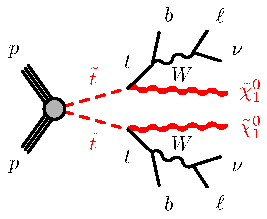
\includegraphics[width=0.3\textwidth]{figures/search_stop2l/signal/fgraph_stop_tN} \hspace{1cm}
        \includegraphics[width=0.3\textwidth]{figures/search_stop2l/signal/fgraph_stop_bCN} \\
        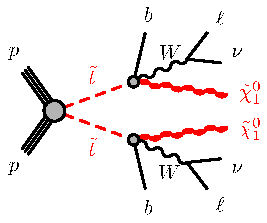
\includegraphics[width=0.3\textwidth]{figures/search_stop2l/signal/fgraph_3body} \hspace{1cm}
        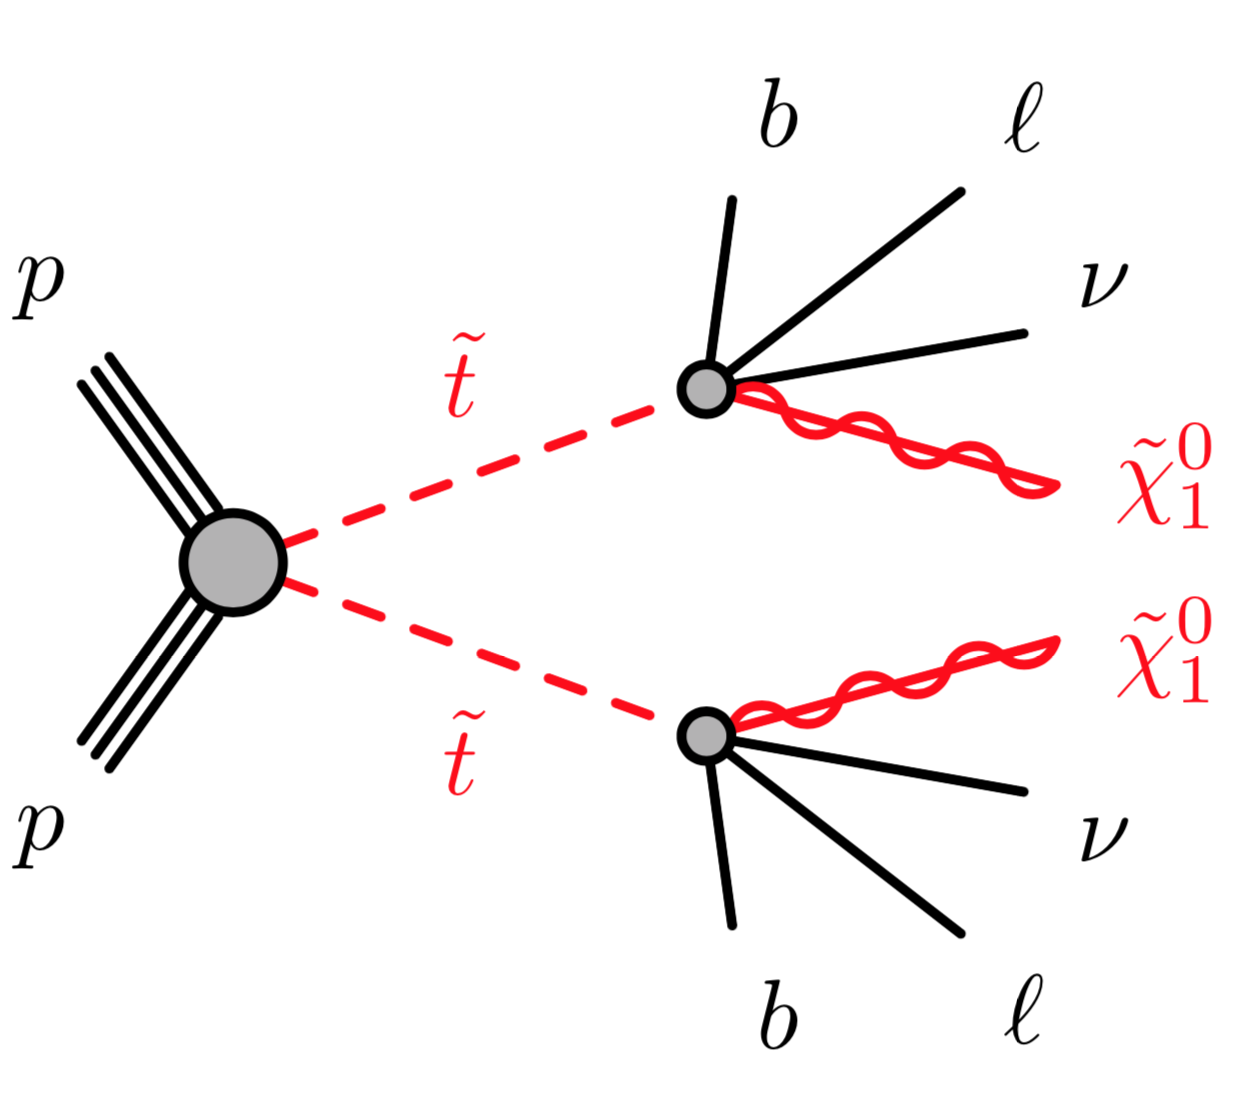
\includegraphics[width=0.3\textwidth]{figures/search_stop2l/signal/fgraph_stop_bffN}
        \caption{
            Decay diagrams for the \stopone relevant to the two-lepton final state of \stopone pair-production.
            \textit{\textbf{Top}}: Diagrams leading to the two-body decay of the \stopone, either
                into $\stopone \rightarrow t \ninoone$ (\textit{top left}) or $\stopone \rightarrow b \chinoonepm$ (\textit{top right}).
            \textit{\textbf{Bottom left}}: Three-body decay of the \stopone, $\stopone \rightarrow b W \ninoone$.
            \textit{\textbf{Bottom right}}: Four-body decay of the \stopone, $\stopone \rightarrow b f f^{\prime} \ninoone$.
        }
        \label{fig:stop_diagrams}
    \end{center}
\end{figure}

\begin{figure}[!htb]
    \begin{center}
        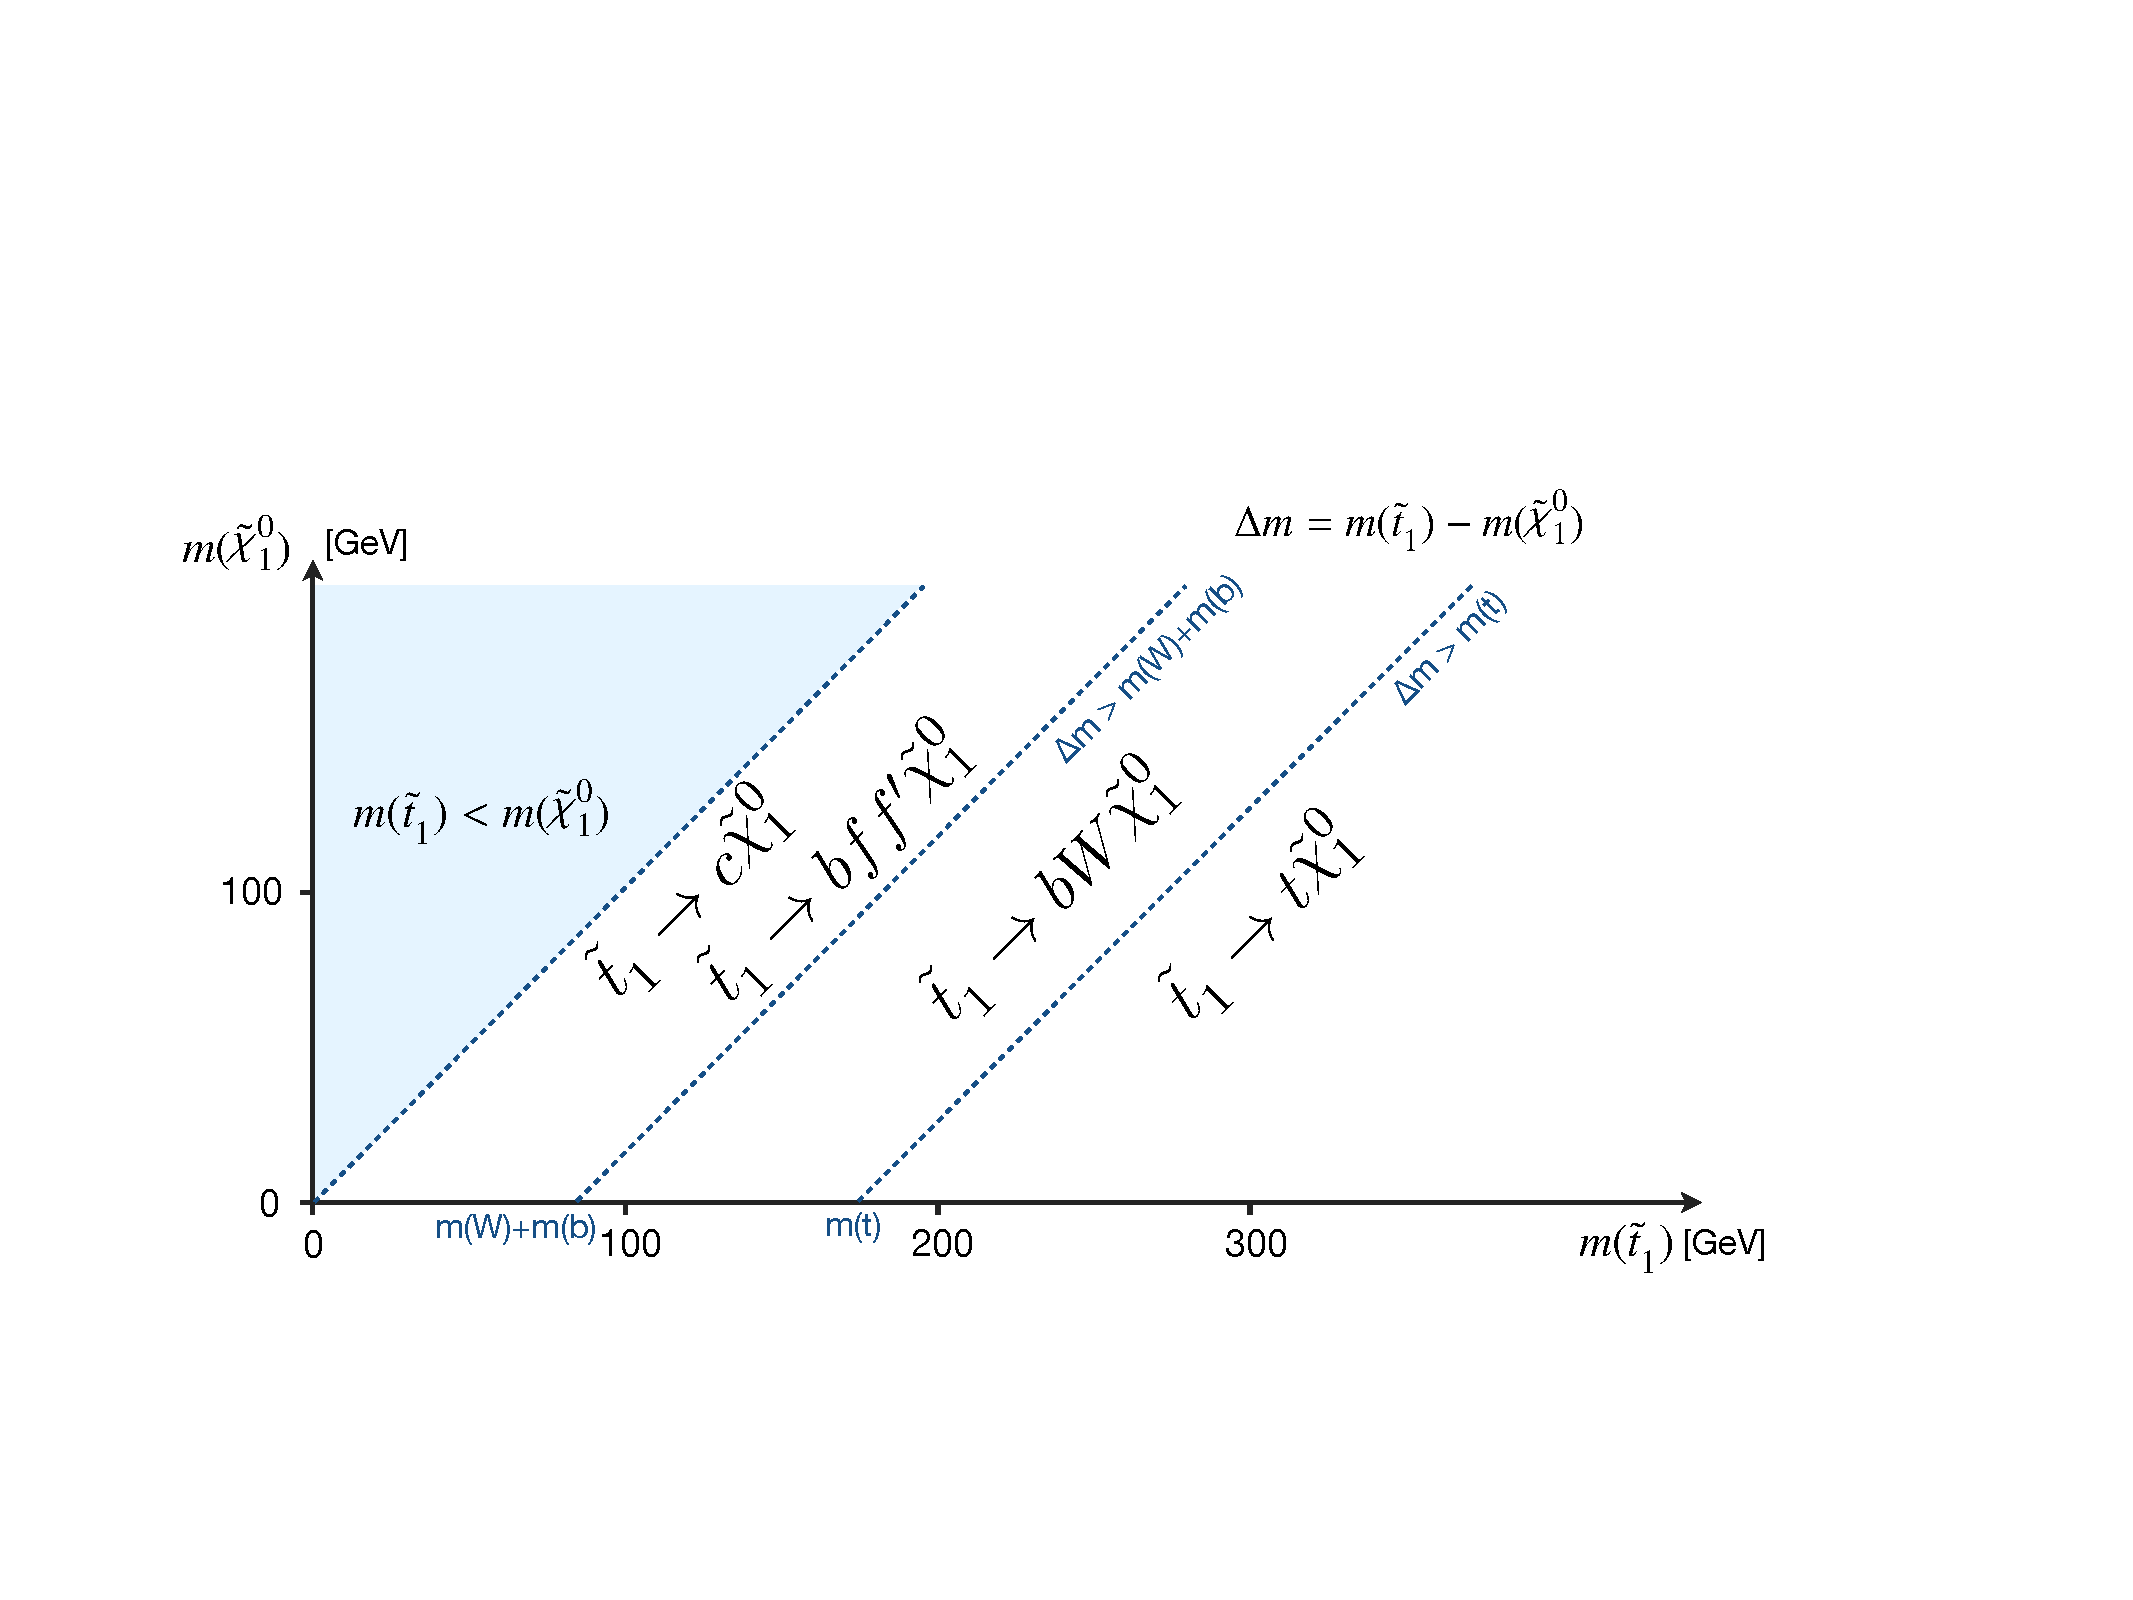
\includegraphics[width=0.7\textwidth]{figures/search_stop2l/signal/stop_LSP_boundaries}
        \caption{
            Kinematic boundaries in the (\stopone,\ninoone) plane, indicating the three kinematic
            regimes associated with the decay of the \stopone: the two-body $\stopone \rightarrow t \ninoone$
            decay ($\Delta m(\stopone, \ninoone) > m_t$), the three-body $\stopone \rightarrow b W \ninoone$ decay
            ($\Delta m(\stopone, \ninoone) < m_t$), and the four-body $\stopone \rightarrow b f f^{\prime} \ninoone$
            decay ($\Delta m(\stopone, \ninoone) < m_b + m_W$).
            Here $\Delta m(\stopone, \ninoone) = m_{\stopone} - m_{\ninoone}$.
        }
        \label{fig:stop_boundaries}
    \end{center}
\end{figure}

Figure~\ref{fig:run1_stop_summary} shows the results of the searches for \stopone particles performed
in Run 1 of the LHC by the ATLAS experiment.
This figure indicates the regions of SUSY parameter space, under the hypothesis of the
simplified model parametrised by the masses of the \stopone and \ninoone particles,
that are excluded at 95\% CL by the zero, one, and two lepton analyses.
It can be seen that the Run 1 analyses targeting the two-lepton final states did not effectively
cover the three-body regime, at least in comparison to all analyses in the two-body and four-body regions
of the $(m_{\stopone}, m_{\ninoone})$-plane.

Section~\ref{sec:susy_exclusion_plots} provides a brief introduction to the type of plots
shown in Figure~\ref{fig:run1_stop_summary}, which are the general SUSY exclusion plots
that are presented to summarise the results of SUSY searches based on simplified models
by both the ATLAS and CMS experiments.
Section~\ref{sec:stop_pheno} then begins by describing the kinematics and phenomenology of the three-body \stopone
decays that are being targeted in the SUSY analysis presented in this chapter.
With the signal kinematics in mind, Section~\ref{sec:stop_event_sel} describes the overall event
selection and object definition used in the analysis, so that the analysis' event sample can be understood.
Section~\ref{sec:stop_strategy} describes how the phenomenology described in Section~\ref{sec:stop_pheno}
motivates a particular choice of discriminating observables that are sensitive to the three-body decay
of the \stopone particle, as well as the definition of the analysis' SRs.
Section~\ref{sec:stop_background_estimate} describes the analysis' background estimation
strategy, particular the definition of CRs and VRs used to constrain the dominant
SM backgrounds.
Section~\ref{sec:stop_results} closes the chapter with the results of the search for
the three-body \stopone in the two-lepton final state.


\begin{figure}[!htb]
    \begin{center}
        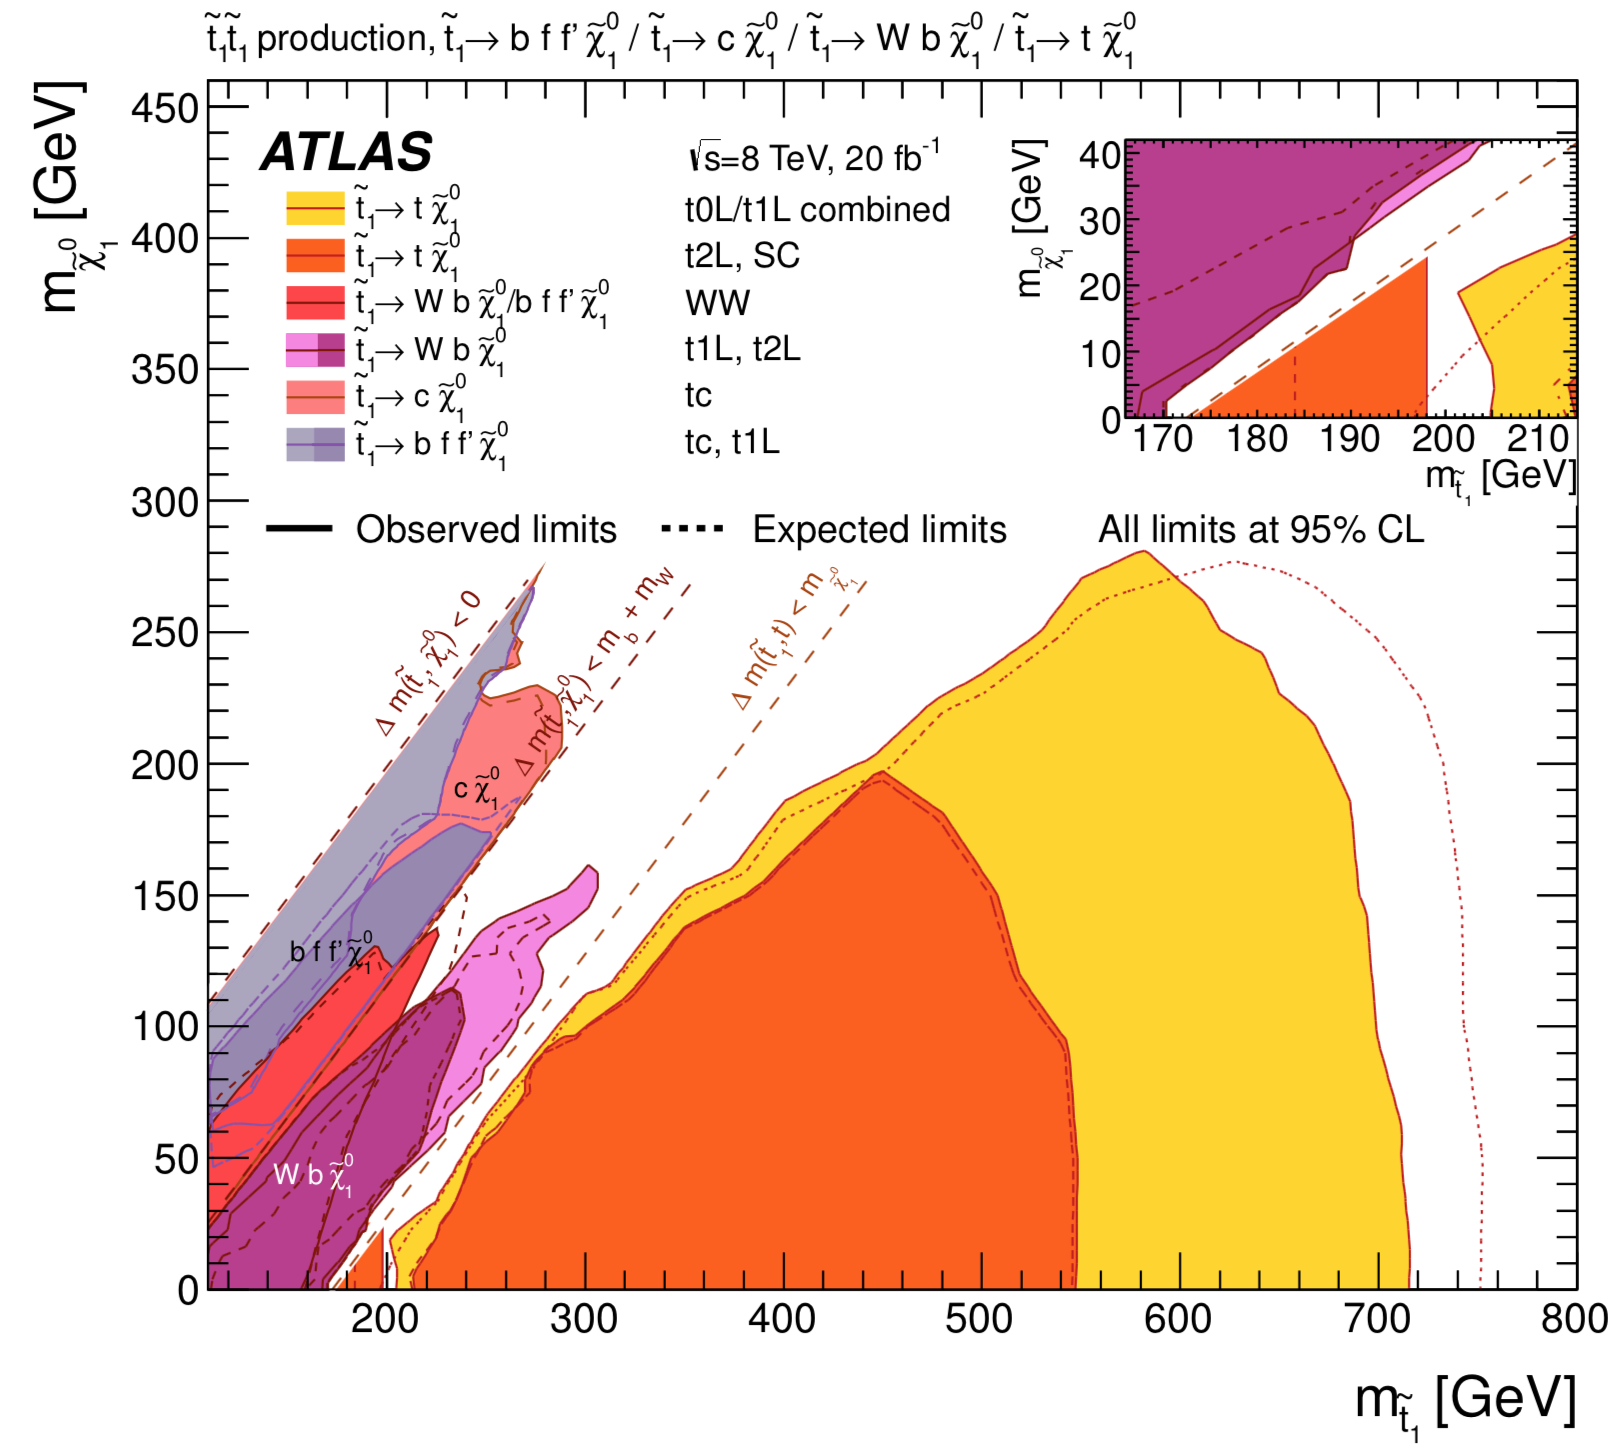
\includegraphics[width=0.7\textwidth]{figures/search_stop2l/run1_stop_summary}
        \caption{
            Summary of SUSY \stopone searches in the (\stopone, \ninoone) plane
            at the end of Run 1.
            The searches relevant to the work in the present thesis are indicated by the 
            coverage of purple and dark orange: `t1L,t2L' and `WW', respectively.
            Figure taken from Ref.~\cite{StopRun1Summary}.
        }
        \label{fig:run1_stop_summary}
    \end{center}
\end{figure}

\FloatBarrier
\section{Aside: SUSY Exclusion Plots}
\label{sec:susy_exclusion_plots}

In this section we describe the typical SUSY exclusion plot, illustrated in Figure~\ref{fig:susy_exclusion_cartoon}.
These plots are used when presenting the results of SUSY searches based on the assumptions
made in simplified models of the MSSM, parametrised only by the masses of the
pair-produced sparticle and the stable sparticle appearing in the final state (the LSP), assuming $R$-parity
conservation. The main things to observe in this plot are as follows:

\begin{enumerate}
    \item The region contained \textit{within} the contours is the region of SUSY parameter space,
        under the assumption of the simplified model, excluded at 95\% CL
    \item The region in which the mass of the produced
        sparticle is less than the mass of the LSP is kinematically forbidden
    \item The analysis sensitivity (i.e. power to exclude) decreases as the mass of the produced sparticle increases
    \item The analysis sensitivity (i.e. power to exclude) decreases as $\sdiff \rightarrow 0$ ($\sdiff \rightarrow m_X$,
        with $m_X$ a mass scale related to an intermediate state appearing in the sparticle decay)
    \item The expected 95\% CL exclusion limits are reported with their $\pm 1 \sigma$ uncertainty band,
        related to the precision of the analyses based on their systematic uncertainty evaluation
    \item The observed 95\% CL exclusion limit is not reported with an error
\end{enumerate}

Item (3) in the above is related to the fact that the cross-section of the SUSY sparticle production cross-section
is a function of only the mass of the pair-produced sparticle in the simplified models assumed here.
The production cross-section decreases in proportion to the mass of the sparticle, indicated in Figure~\ref{fig:susy_xsec},
which leads to analyses becoming less sensitive to the scenarios with larger masses of the produced sparticles.

Item (4) is also relatively straightforward.
As the masses of the produced sparticle and final-state LSP become nearer to one another, and even
degenerate, kinematic phase space suppression results in there being less energy-momentum available to be transferred to the final state
particles.
This results in final state particles having typically lower energies and momenta,
making them difficult to trigger on and reconstruct efficiently.
This inefficiency reduces an analysis' sensitivity to these kinematic regimes, since the final states become experimentally
inaccessible.
This scenario also appears when the produced sparticle follows a more complex decay chain,
as in the cases illustrated in Figure~\ref{fig:stop_diagrams}, where intermediate mass scales such as the
mass of the SM top-quark or $W$-boson are introduced.
Near these regions, the kinematics of the particles decaying from the objects defining these intermediate
mass scales change rapidly.
As a result, analyses targeting particle kinematics on one side of such a boundary
cannot simultaneously be sensitive to the particle kinematics on the opposing side of the boundary.
For this reason, it is common practice to define separate analyses targeting each side of a given boundary,
as indicated in Figure~\ref{fig:run1_stop_summary}.

The expected limits in Item (5) in the above are related to running the analysis' hypothesis tests
on the SUSY scenarios indicated by the position on the $(m_{\stopone}, m_{\ninoone})$-plane,
and using for $\bm{N^{\text{obs}}}$ (c.f. Equations~\ref{eq:likelihood_main} and \ref{eq:full_likelihood}) the value in the SRs for the predicted background; that is, the
observed data counts in the analysis' signal regions are substituted with the value of the total predicted
background in the signal regions.
The observed data is still used in the CRs, which provide the normalisation correction factors as described in Section~\ref{sec:likelihood}.
The observed limits discussed in Item (6), on the other hand, take as $\bm{N^{\text{obs}}}$ the actual observed data counts
in the analysis' SRs.
Due to statistical fluctuations in the observed data, the expected and observed 95\%CL exclusion contours
do not typically overlap perfectly.

\begin{figure}[!htb]
    \begin{center}
        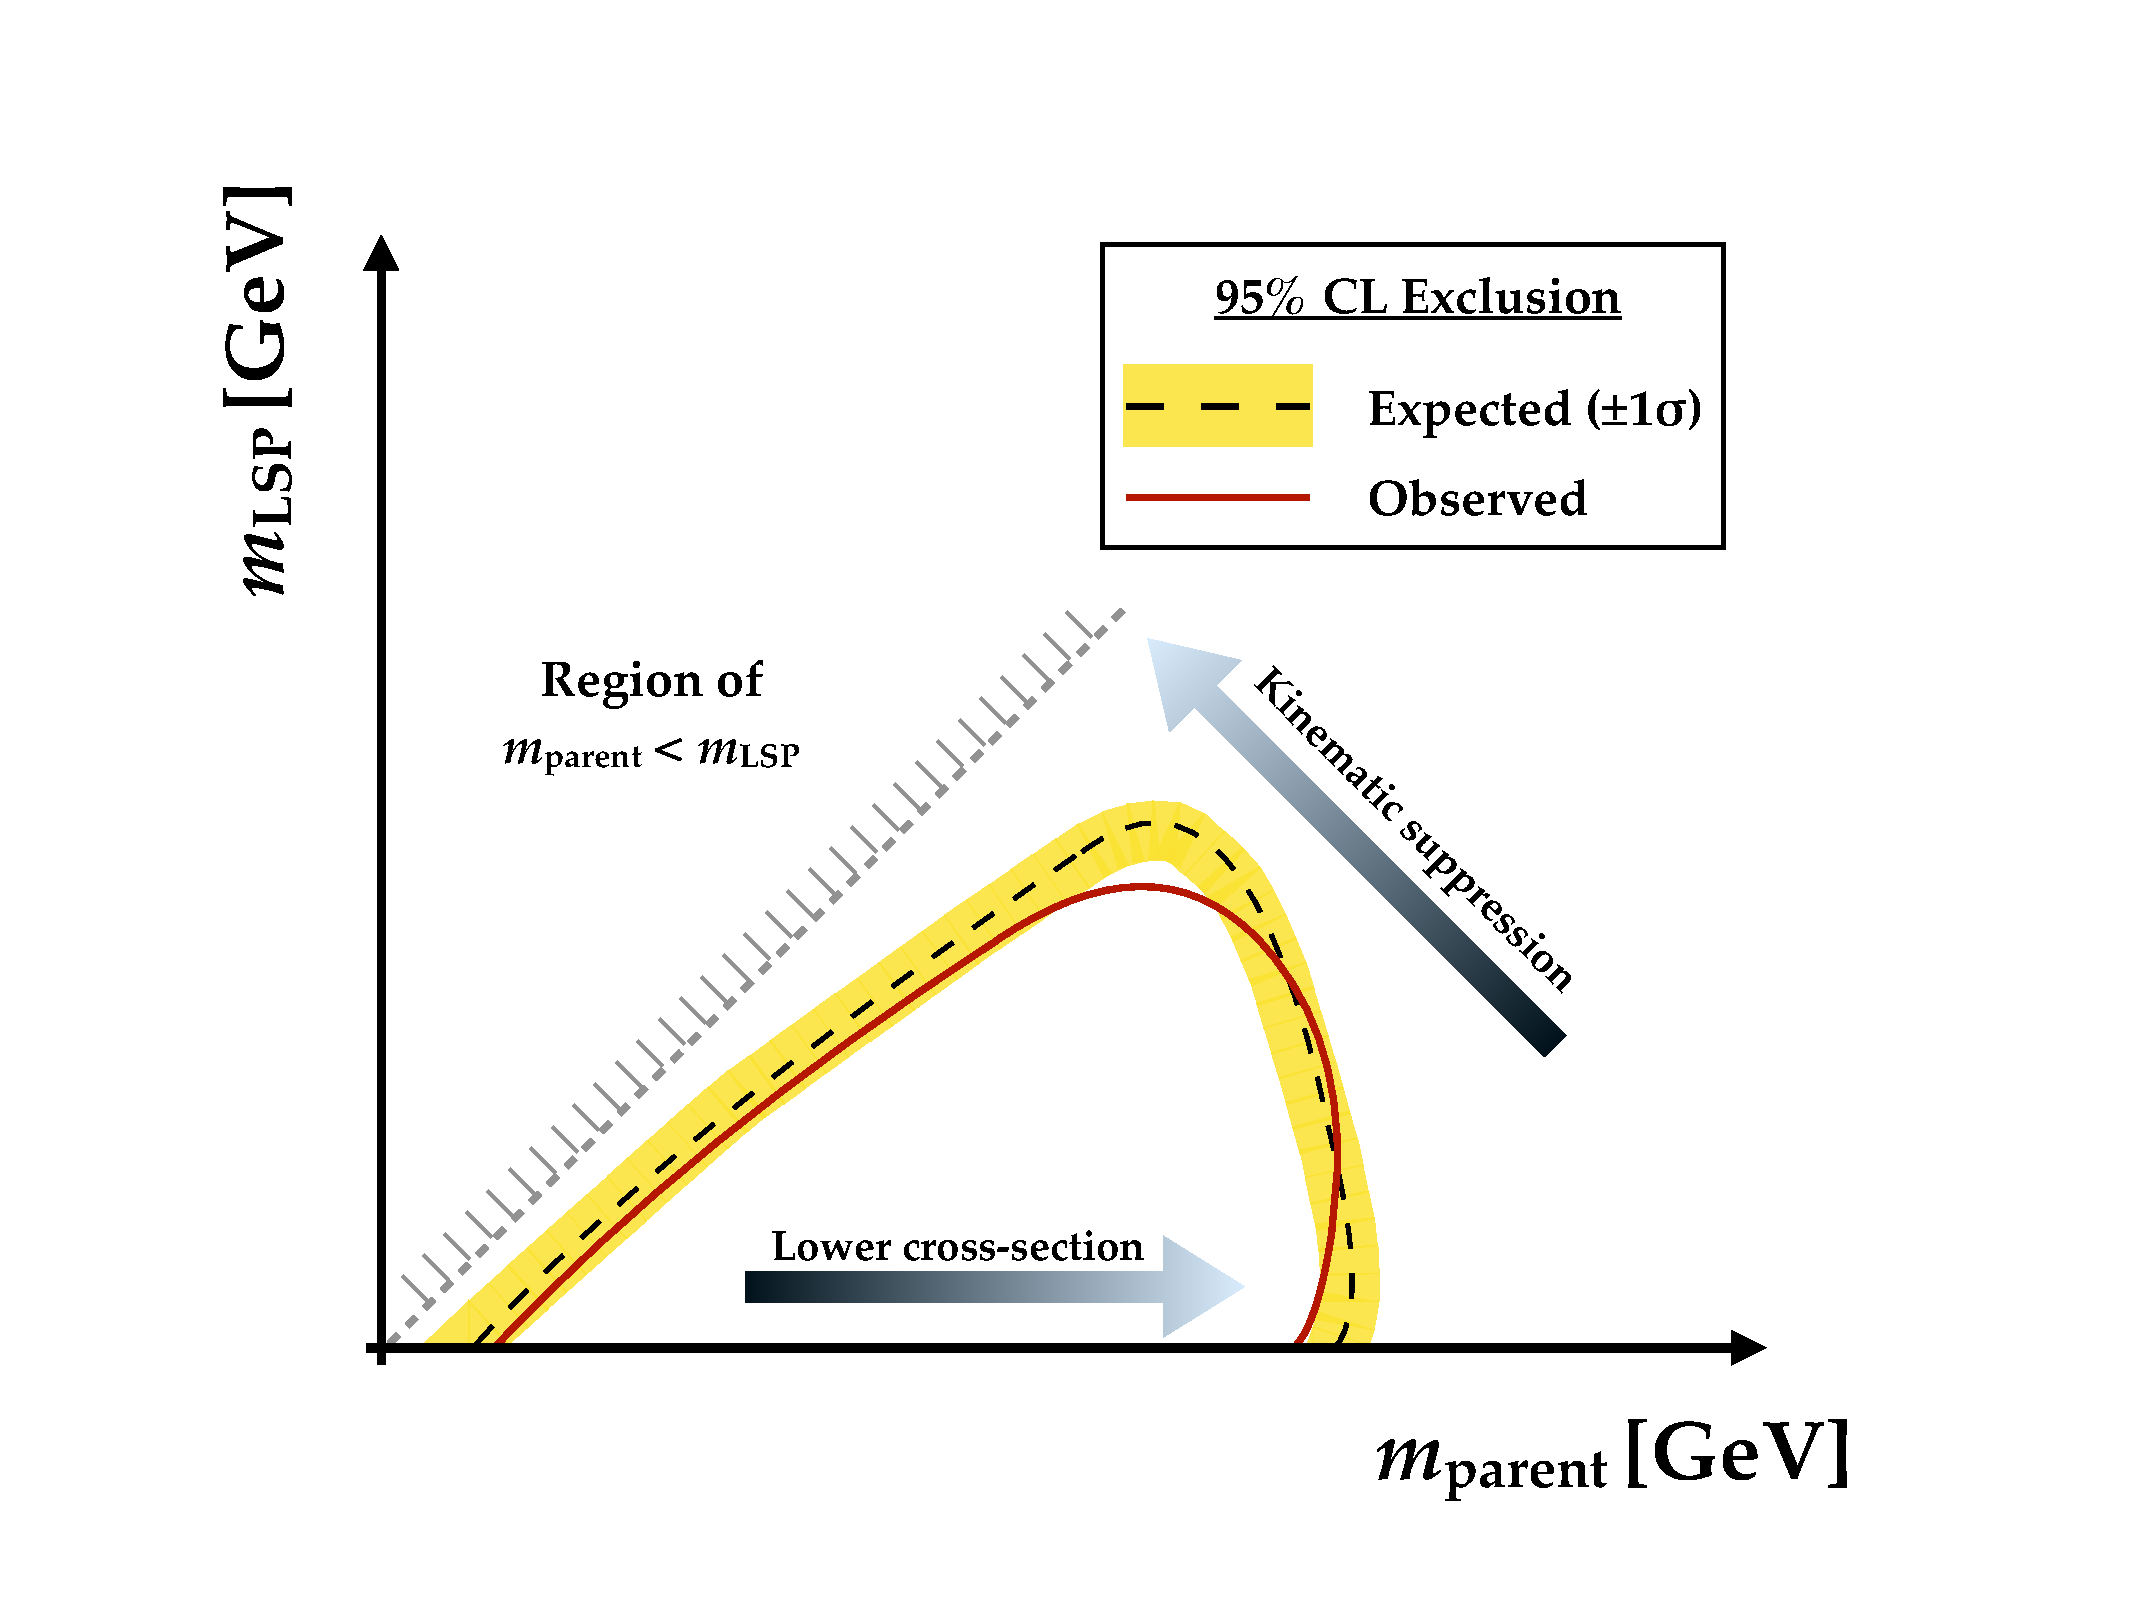
\includegraphics[width=0.8\textwidth]{figures/search_stop2l/susy_exclusion_cartoonPDF}
        \caption{
            Cartoon illustrating an example of a typical two-dimensional exclusion plot
            for a SUSY simplified model.
            The mass of the pair-produced SUSY particle is on the $x$-axis and the mass of the
            LSP to which it decays is on the $y$-axis.
            The region bounded by (i.e. inside of) the dashed-black (red) curves indicate
            the expected (observed) region of SUSY parameter space excluded at the 95\% CL.
            The $\pm 1\sigma$ error band is shown on the expected limits, and is based on the
            systematic uncertainties included in the analysis.
            SUSY exclusion curves such as these usually exhibit a triangular shape as a result
            of two competing effects, indicated by the arrows: 1) the reduction in production
            cross-section as the mass of the produced SUSY particle increases, and 2) kinematic
            suppression occurring when the phase space available to the final state decreases
            as a result of $\Delta m (x, y) = m_x - m_y \rightarrow 0$.
            Kinematic suppression results in the final state objects, such as leptons and $b$-tagged jets
            in the case presented in the current thesis,
            having very little momenta, thereby making it difficult to efficiently identify
            the event as being consistent with the given SUSY hypothesis being searched for.
        }
        \label{fig:susy_exclusion_cartoon}
    \end{center}
\end{figure}

\begin{figure}[!htb]
    \begin{center}
        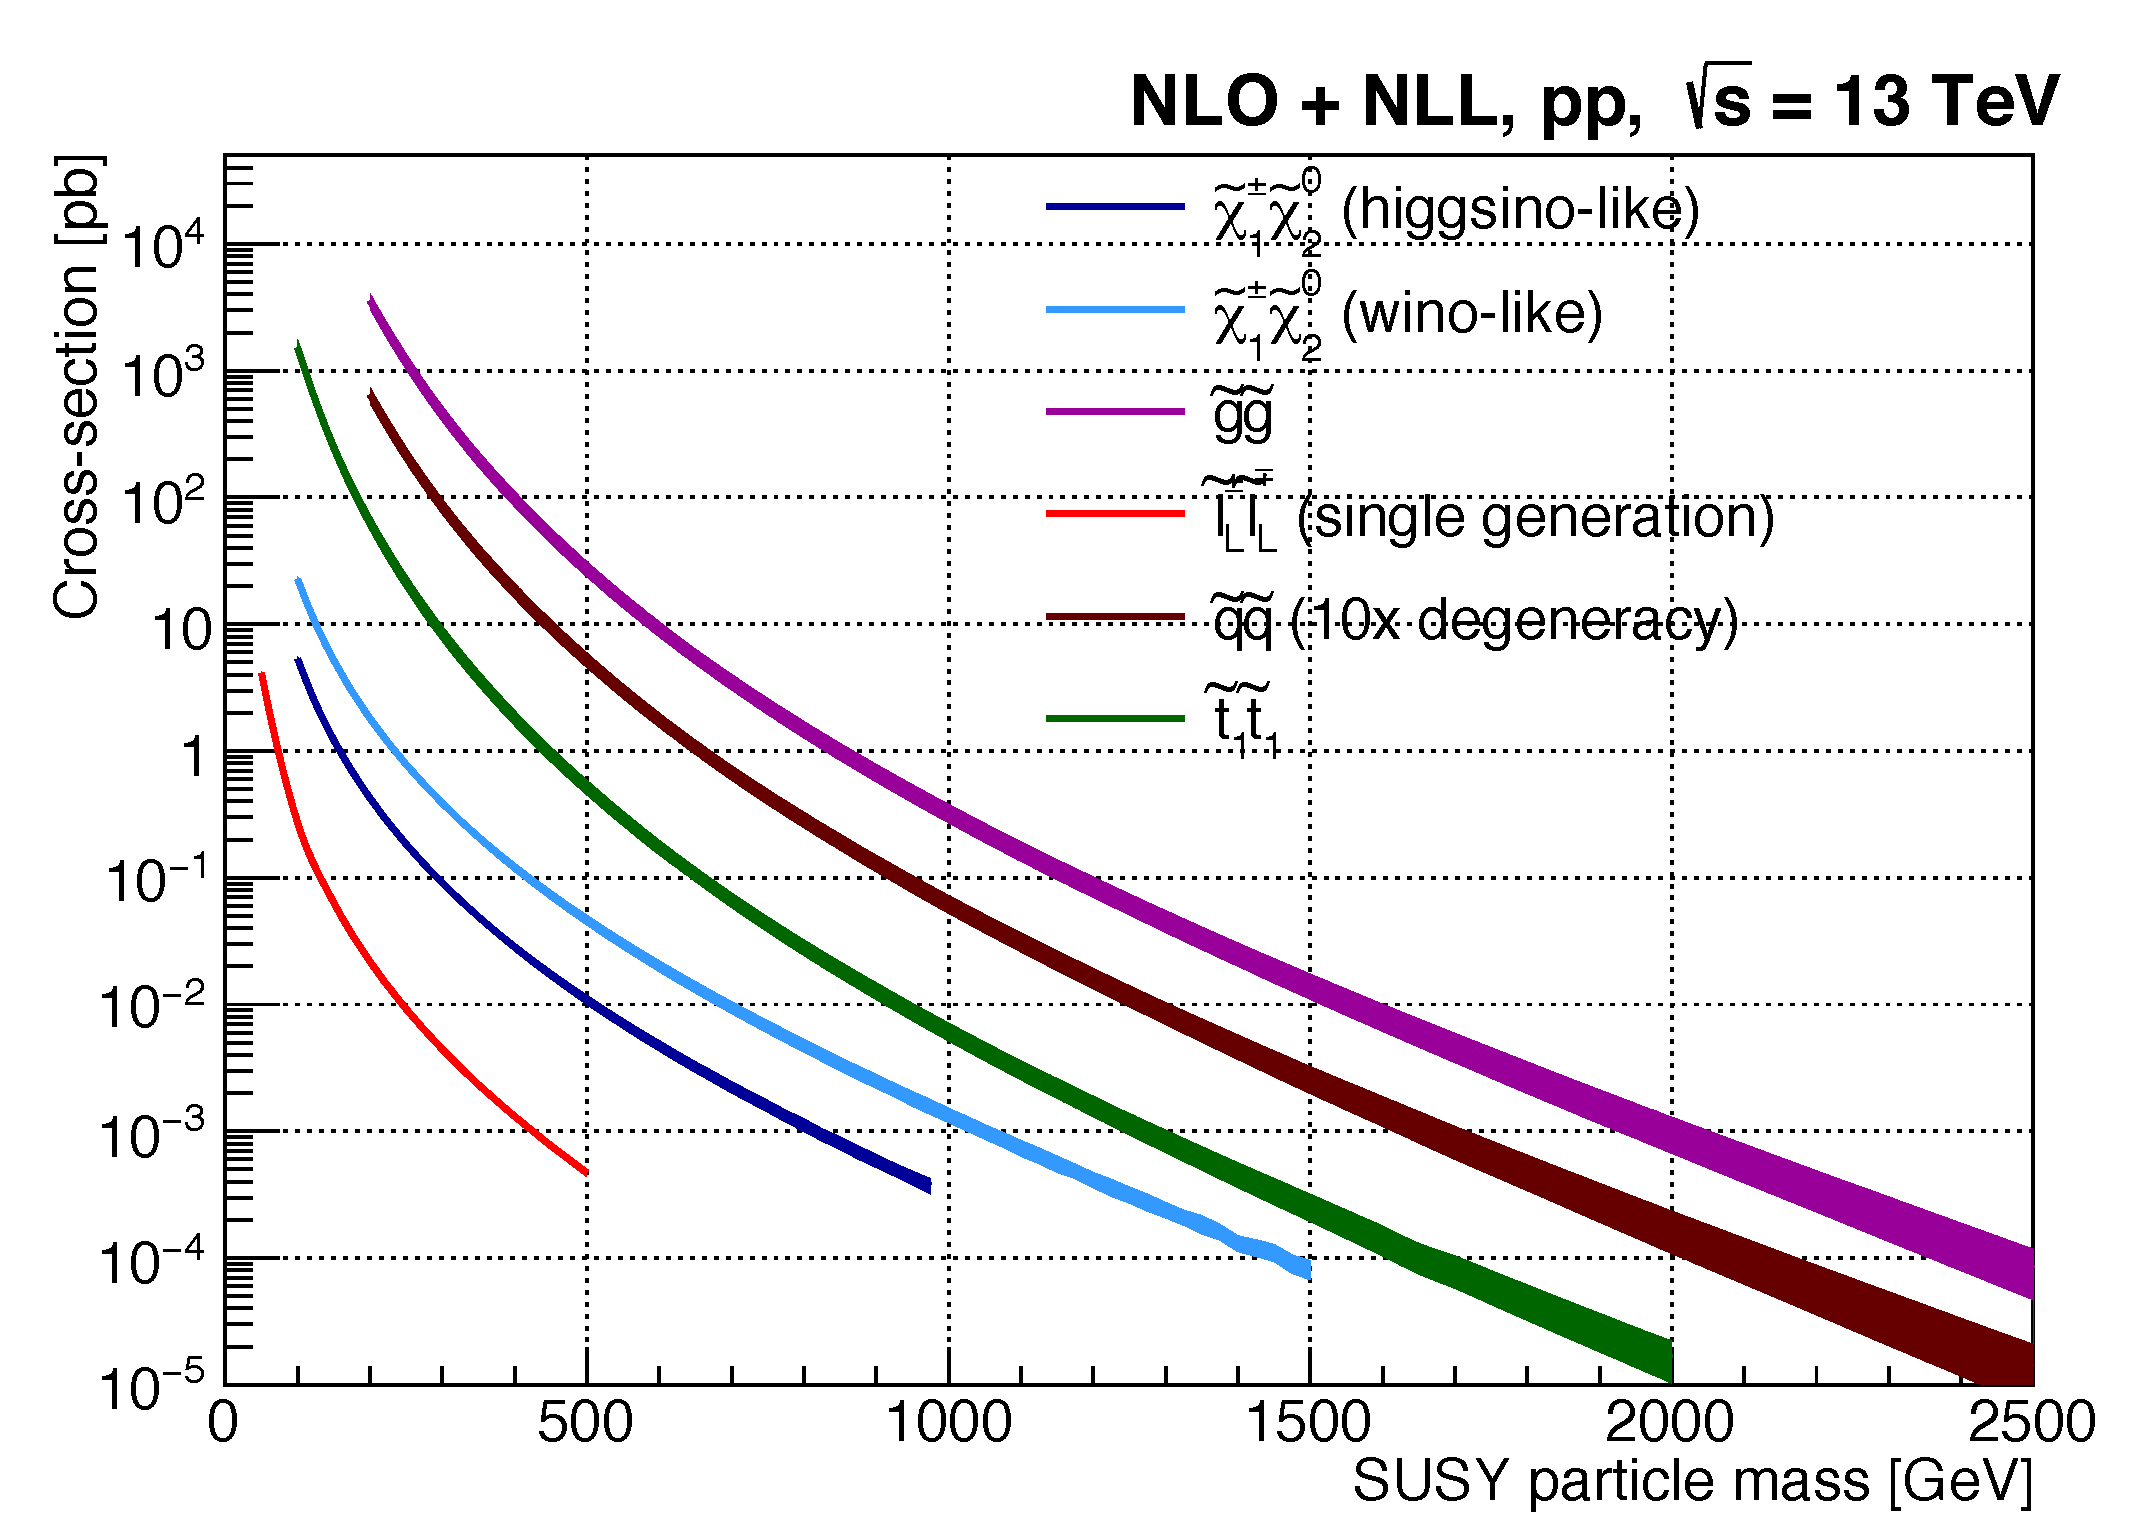
\includegraphics[width=0.65\textwidth]{figures/search_stop2l/SUSY_xsec_13TeV_v1}
        \caption{
            Production cross-section for the SUSY sparticles indicated in the legend,
            as a function of their mass, computed as in Ref.~\cite{SUSYXsec1}.
            The bands indicate the uncertainty due to the theoretical prediction of the production
            process.
            The green band indicates the \stopone production cross-section, relevant to the analysis
            described in the current chapter.
            For comparison, the production cross-section for SM top-quark pair-production is $\approx 830$\,pb at 13\,\TeV.
        }
        \label{fig:susy_xsec}
    \end{center}
\end{figure}

\FloatBarrier
%%%%%%%%%%%%%%%%%%%%%%%%%%%%%%%%%%%%%%%%%%%%%%%%%%%%%%%%%%%%%%%%%%%%%%%%%%%
%%%%%%%%%%%%%%%%%%%%%%%%%%%%%%%%%%%%%%%%%%%%%%%%%%%%%%%%%%%%%%%%%%%%%%%%%%%
%%%%%%%%%%%%%%%%%%%%%%%%%%%%%%%%%%%%%%%%%%%%%%%%%%%%%%%%%%%%%%%%%%%%%%%%%%%
%
% SIGNAL DESCRIPTION
%
%%%%%%%%%%%%%%%%%%%%%%%%%%%%%%%%%%%%%%%%%%%%%%%%%%%%%%%%%%%%%%%%%%%%%%%%%%%
%%%%%%%%%%%%%%%%%%%%%%%%%%%%%%%%%%%%%%%%%%%%%%%%%%%%%%%%%%%%%%%%%%%%%%%%%%%
%%%%%%%%%%%%%%%%%%%%%%%%%%%%%%%%%%%%%%%%%%%%%%%%%%%%%%%%%%%%%%%%%%%%%%%%%%%
\section{The Dilepton $hh \rightarrow \bbww$ Signal Process}
\label{sec:hh_pheno}

{\color{red}{MENTION SCALAR WW DECAY AND WW SPIN CORRELATION THAT ONLY THE DILEPTON CHANNEL CAN TAKE ADVANTAGE OF}}

In the dilepton decay of the $hh \rightarrow \bbww$ channel, the $WW^*$ system
cannot be fully reconstructed in order to produce, for example, a $WW^*$ invariant
mass observable that has a resonance structure at $m_h = 125$\,GeV.
This is due to the
kinematically under-constrained final state in which the \met is a result of the double neutrino system
arising from the leptonically decaying $W$ bosons.
Additionally, the final state is the same as that of SM \ttbar~production.
As a result, the dominant SM background to the analysis is expected to be SM \ttbar~and top-quark processes.

There are crucial \textit{topological} differences between the observable final states of dilepton SM \ttbar~production and
that of \bbww, however.
The dileptonic \bbww final state is characterised by `Higgs hemispheres'.
One hemisphere contains the two $b$-tagged jets from the $h \rightarrow bb$ decay and is generally
opposite in the transverse ($xy$) plane to the second hemisphere that contains the two leptons
and \met from the $h \rightarrow WW^*$ decay.
In the case of \ttbar, the $b$-tagged jets, leptons, and neutrinos tend to be distributed more uniformly
within the event, leading to events that do not typically exhibit the same back-to-back hemispheres
topology as the \bbww signal process.
This is illustrated in Figure~\ref{fig:hh_topo}.

The presence of these Higgs hemispheres in the signal, in which the momentum flow of the $WW^*$ system
is correlated with that of the $bb$ system's, will be relied upon to inform the analysis' choice
of kinematic observables that are sensitive to the dilepton $hh \rightarrow \bbww$ signal process.

\begin{figure}[!htb]
    \begin{center}
        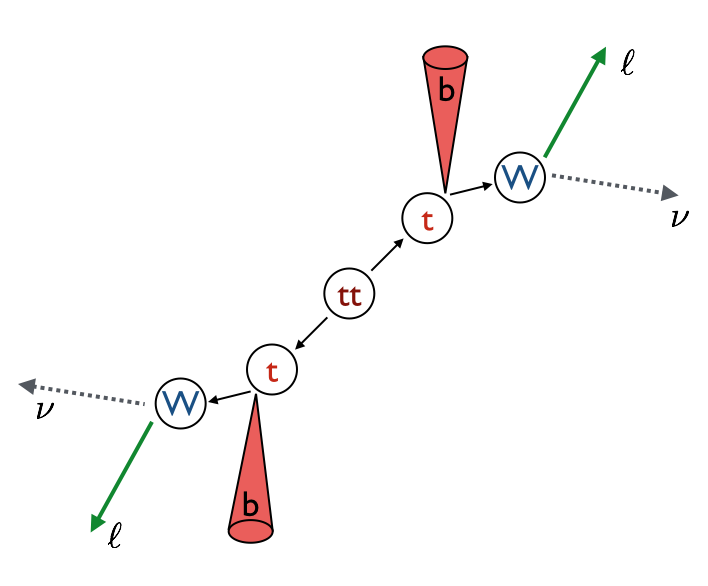
\includegraphics[width=0.52\textwidth]{figures/search_hh/signal_pheno/ttbar_topo}
        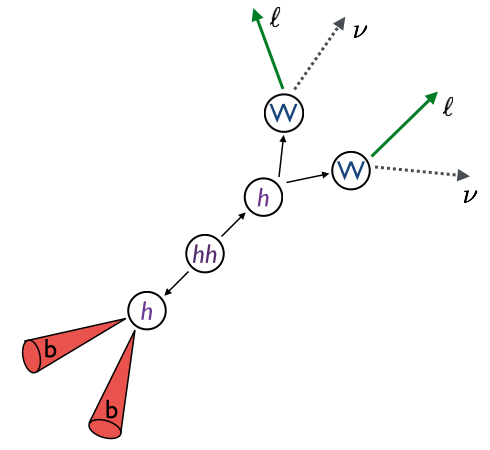
\includegraphics[width=0.46\textwidth]{figures/search_hh/signal_pheno/hh_topo}
        \caption{
            Dilepton $bbWW$ shapes.
            \textit{\textbf{Left}}: SM top-quark pair production.
            \textit{\textbf{Right}}: $hh \rightarrow \bbww$.
        }
        \label{fig:hh_topo}
    \end{center}
\end{figure}

%%%%%%%%%%%%%%%%%%%%%%%%%%%%%%%%%%%%%%%%%%%%%%%%%%%%%%%%%%%%%%%%%%%%%%%%%%%%%%%%%%%
%%%%%%%%%%%%%%%%%%%%%%%%%%%%%%%%%%%%%%%%%%%%%%%%%%%%%%%%%%%%%%%%%%%%%%%%%%%%%%%%%%%
%%%%%%%%%%%%%%%%%%%%%%%%%%%%%%%%%%%%%%%%%%%%%%%%%%%%%%%%%%%%%%%%%%%%%%%%%%%%%%%%%%%
%
% KINEMATIC DISTRIBUTIONS/SHAPES
%
%%%%%%%%%%%%%%%%%%%%%%%%%%%%%%%%%%%%%%%%%%%%%%%%%%%%%%%%%%%%%%%%%%%%%%%%%%%%%%%%%%%
%%%%%%%%%%%%%%%%%%%%%%%%%%%%%%%%%%%%%%%%%%%%%%%%%%%%%%%%%%%%%%%%%%%%%%%%%%%%%%%%%%%
%%%%%%%%%%%%%%%%%%%%%%%%%%%%%%%%%%%%%%%%%%%%%%%%%%%%%%%%%%%%%%%%%%%%%%%%%%%%%%%%%%%

In the following we present some kinematic distributions illustrating the unique topologies
of the dilepton $hh \rightarrow \bbww$ signal process as compared to the dominant top-quark background
processes.

Figure~\ref{fig:hh_kin_0} shows distributions related to the $bb$ system.
It can be seen from the $|\dphibb|$ and \drbb distributions that the two $b$-tagged jets
are collinear in the signal process as compared to the background processes.
For the \ttbar~background, these tendencies in $|\dphibb|$ and \drbb are reversed,
as expected from their different topology with the $b$-tagged jets on opposing sides of the event.
For single-top $Wt$, similar trends as observed in \ttbar are observe but, since the second $b$-tagged
jet in the $Wt$ process is due to higher-order contributions (or a light-flavor jet mistakenly identified as a $b$-jet),
the $b$-tagged jets are often more collinear.

Figure~\ref{fig:hh_kin_1} shows a few distributions related to the dilepton, \met, and $\met$ + dilepton systems.
We can see from the $|\dphimetll|$ and \drll distributions that for the signal $hh$ process, the leptons
are collinear as expected, with the leptons contained almost entirely within a cone of radius $\drll = 1$.
For the top-quark backgrounds, there is a tendency for the leptons to be back-to-back, with $|\dphill| (\drll) \rightarrow \pi$.

The $|\Delta \phi|$ between the \met and dilepton system, $|\dphimetll|$, shows that the $WW^*$ system is collinear, as well.
For the SM top-quark backgrounds, $|\dphimetll|$ tends slowly towards $\pi$.
In the case of single-top $Wt$, however, there is a tendency for $|\dphimetll|$ to gather towards lower values due
to similar effects as described previously: the more collinear $b$-tagged jets force the
$WW^*$ system to also become collinear so that it balances the $bb$ system.

\begin{figure}[!htb]
    \begin{center}
        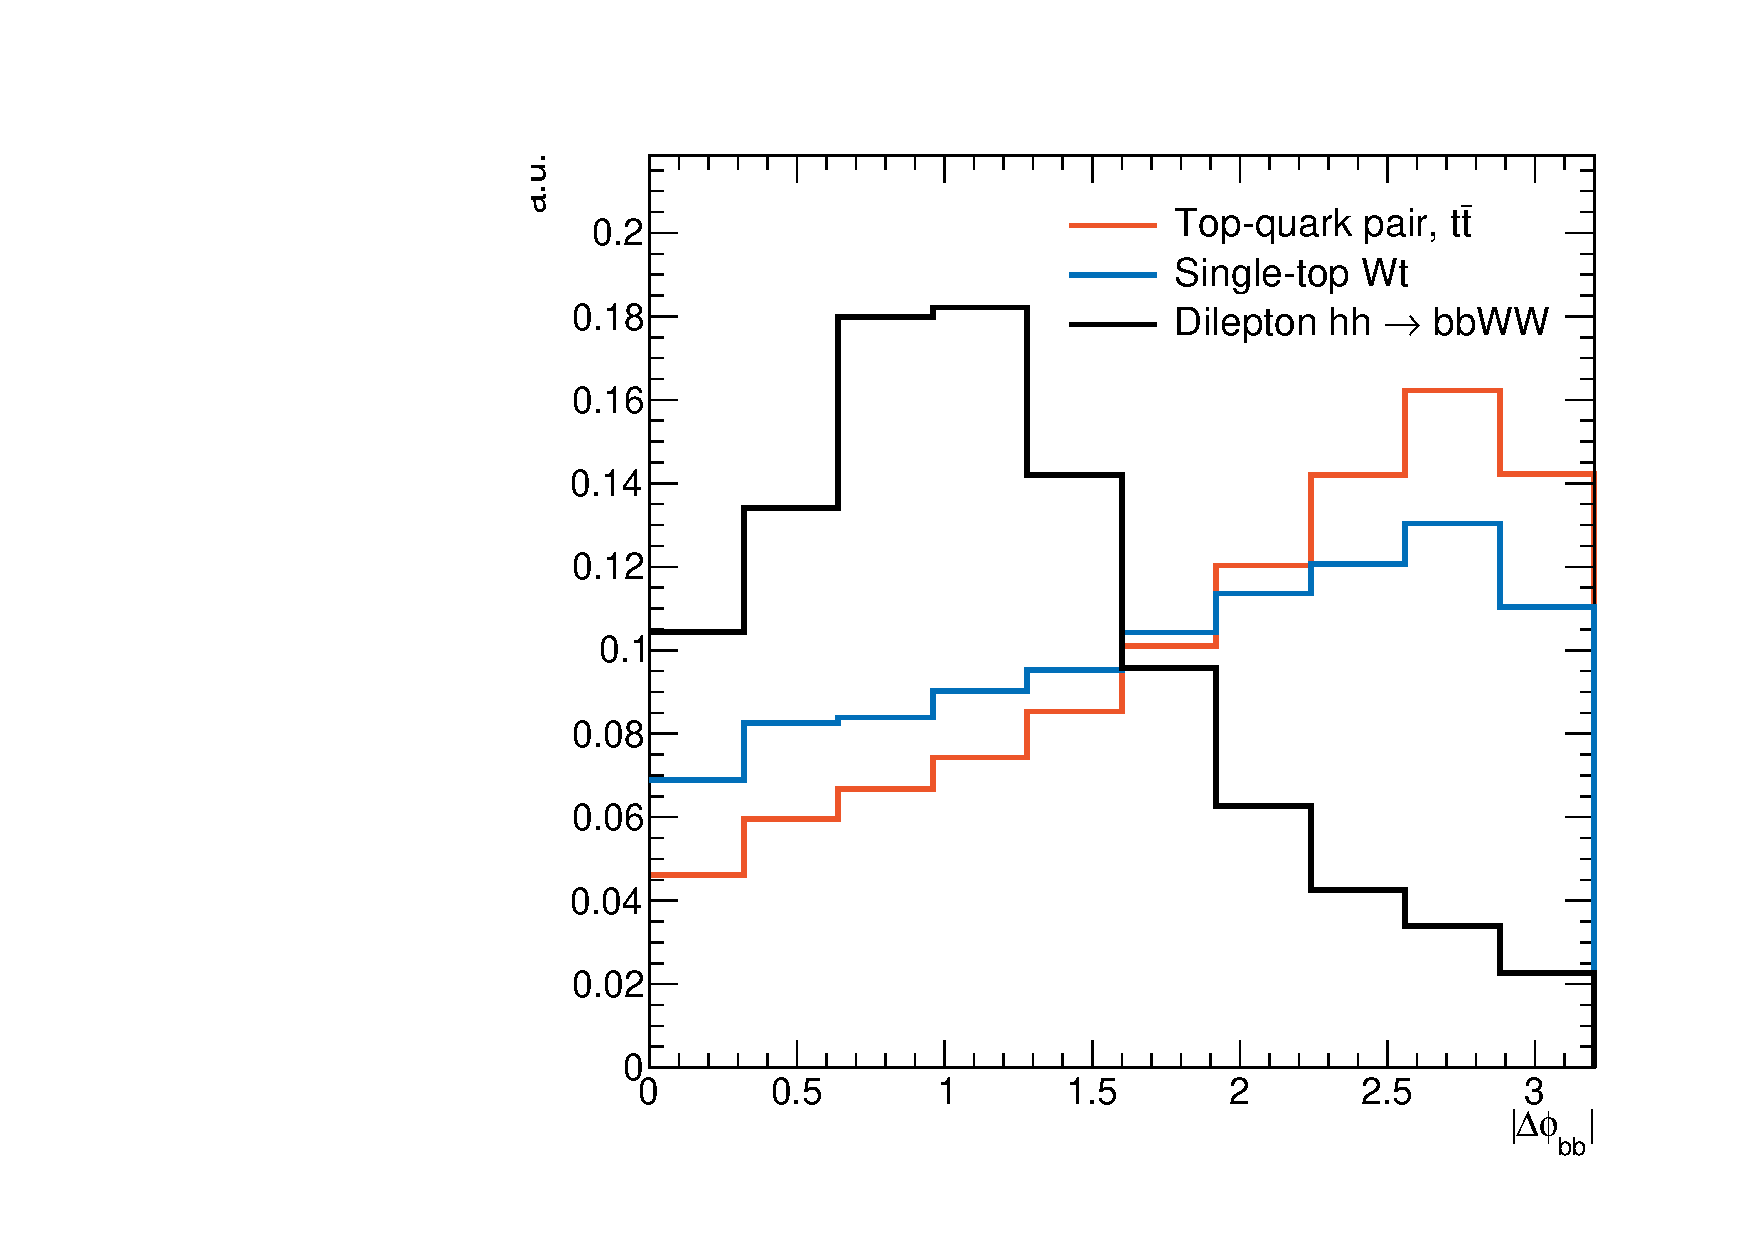
\includegraphics[width=0.45\textwidth]{figures/search_hh/signal_pheno/shape_plots/hh_shape_plot_dphi_bb}
        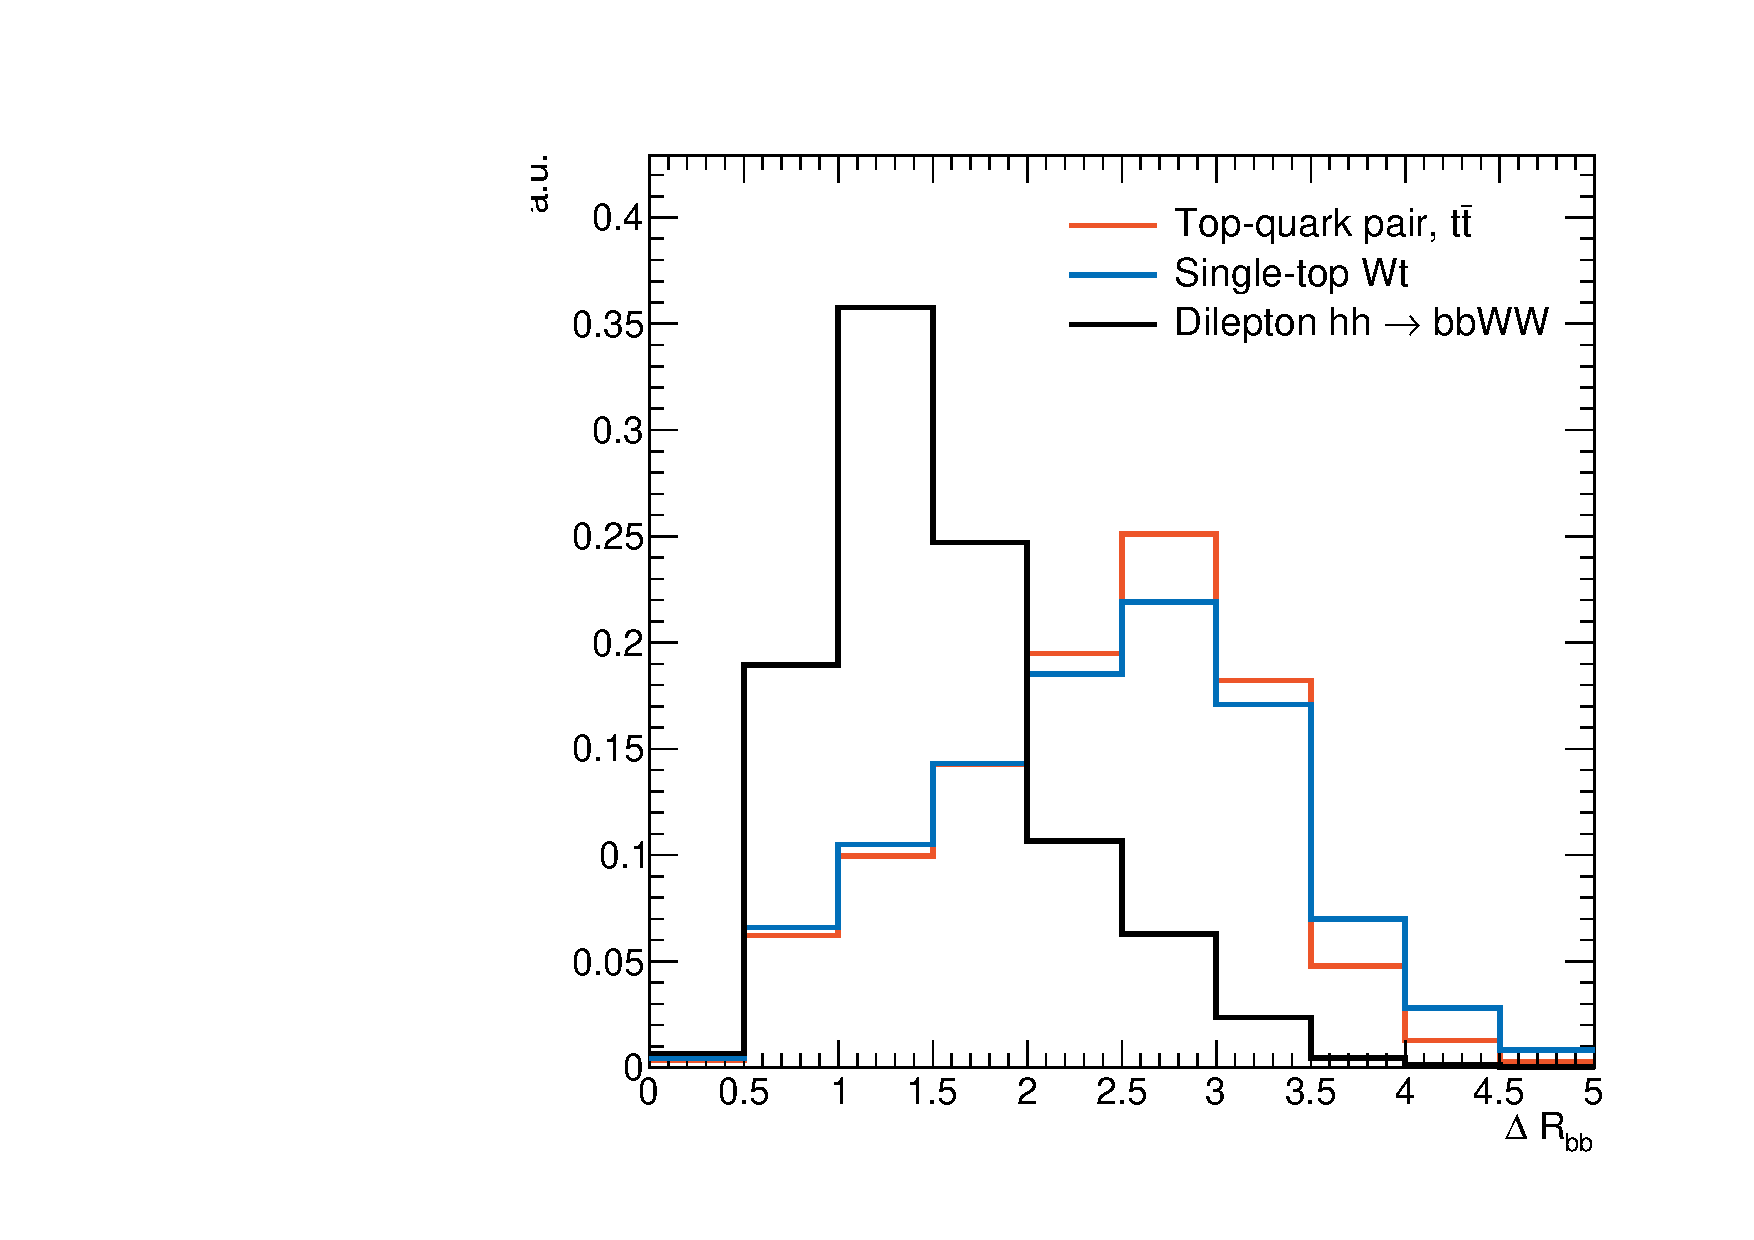
\includegraphics[width=0.45\textwidth]{figures/search_hh/signal_pheno/shape_plots/hh_shape_plot_dRbb}
        \caption{
            Normalized distributions showing the shapes of kinematic distributions for the SM
            top-quark processes (\ttbar~and single-top $Wt$) and the dilepton $hh \rightarrow \bbww$ signal process.
            \textit{\textbf{Left}}: $|\Delta \phi|$ between the two $b$-tagged jets, $|\dphibb|$.
            \textit{\textbf{Right}}: $\Delta R$ between the two $b$-tagged jets, $\drbb$.
        }
        \label{fig:hh_kin_0}
    \end{center}
\end{figure}

\begin{figure}[!htb]
    \begin{center}
        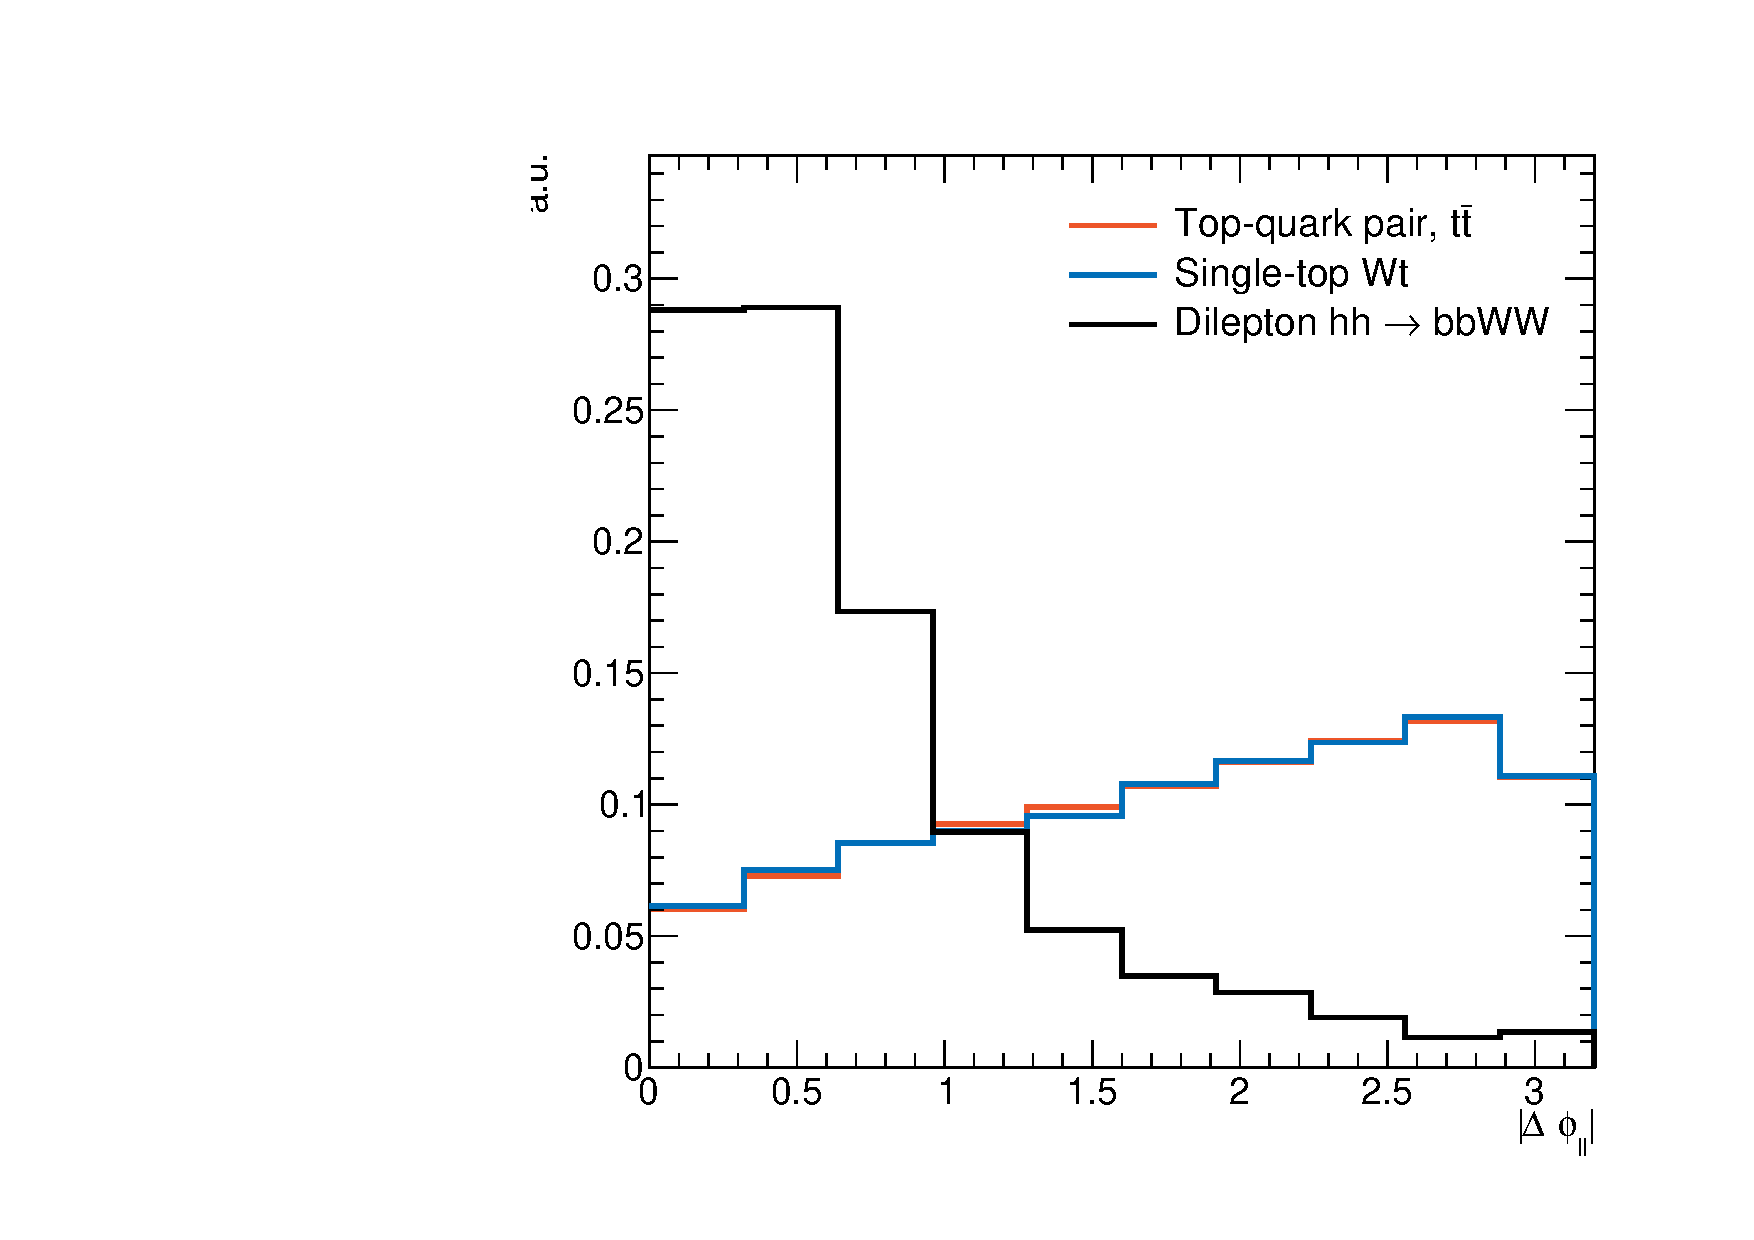
\includegraphics[width=0.45\textwidth]{figures/search_hh/signal_pheno/shape_plots/hh_shape_plot_dphi_ll}
        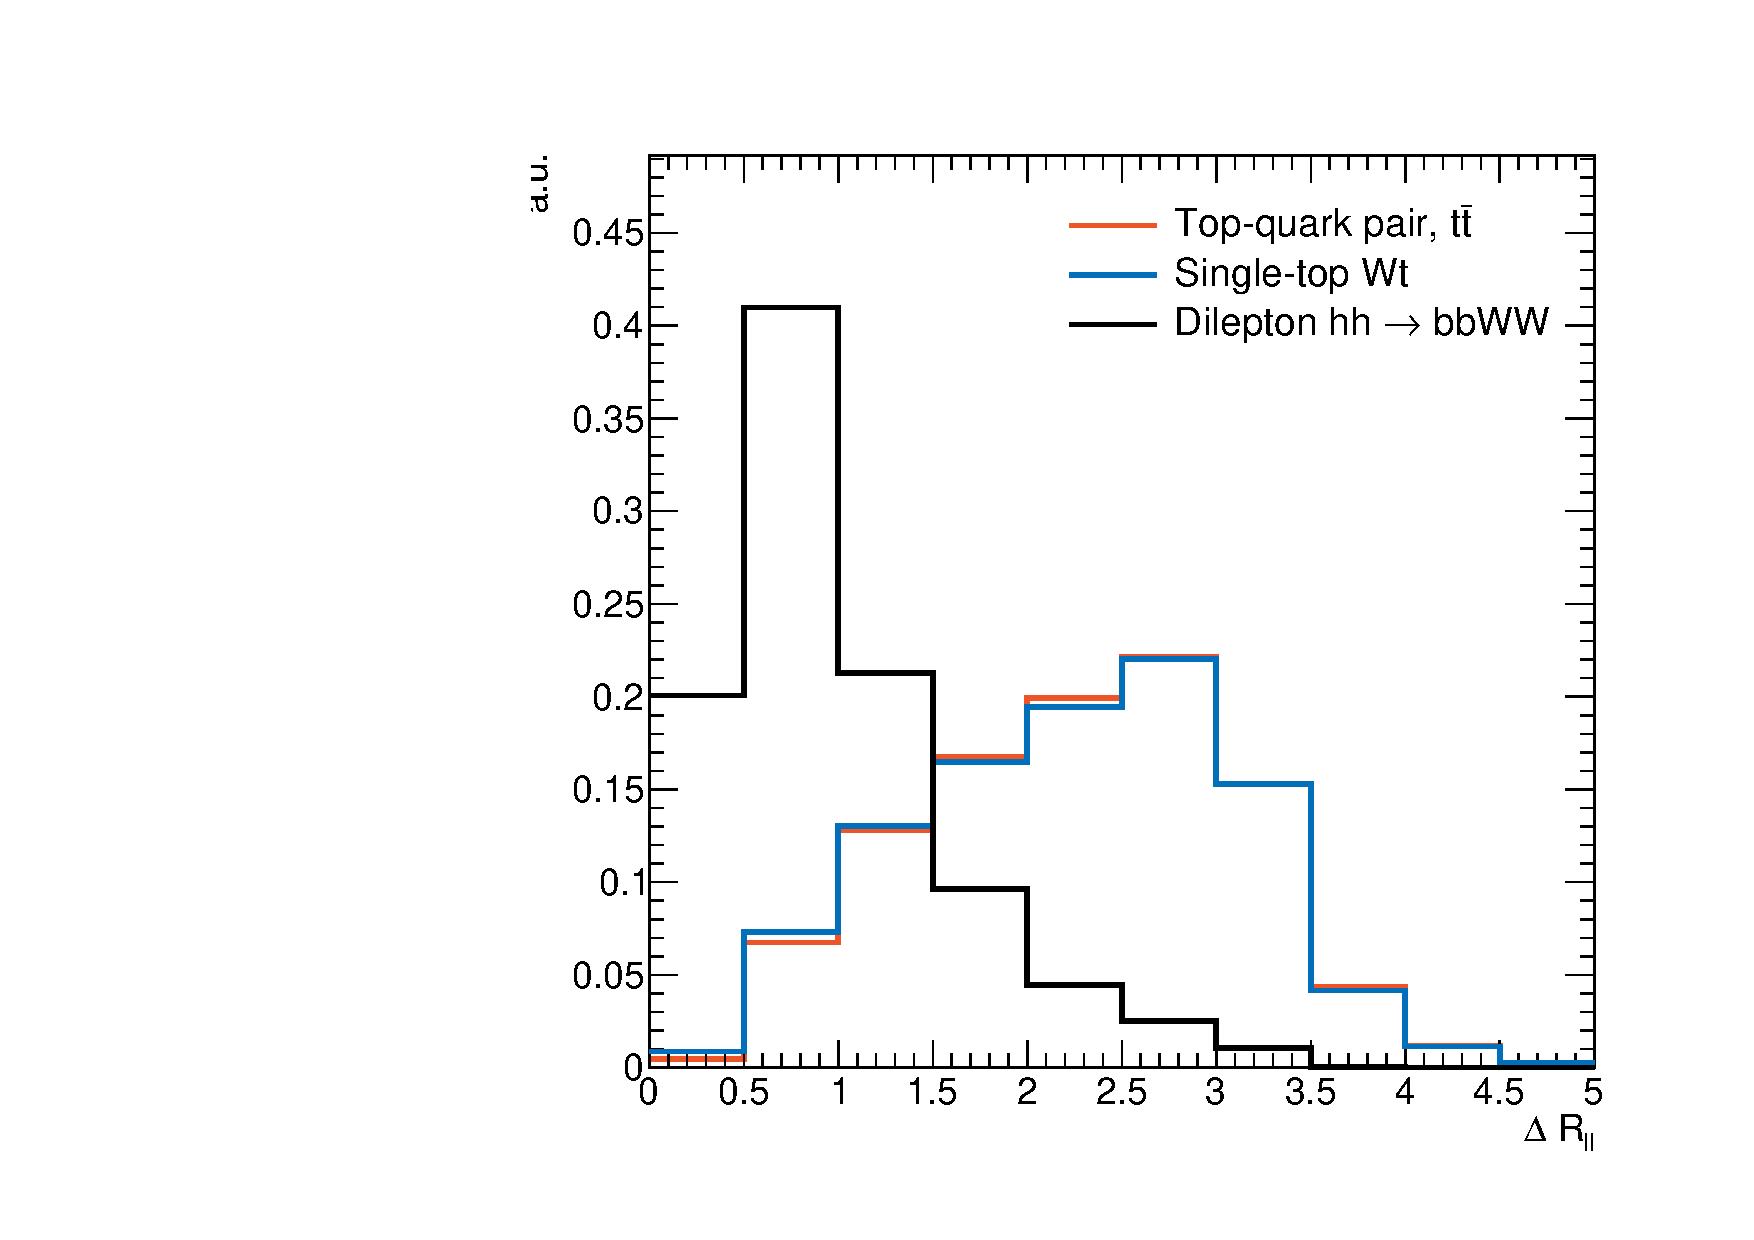
\includegraphics[width=0.45\textwidth]{figures/search_hh/signal_pheno/shape_plots/hh_shape_plot_dRll}
        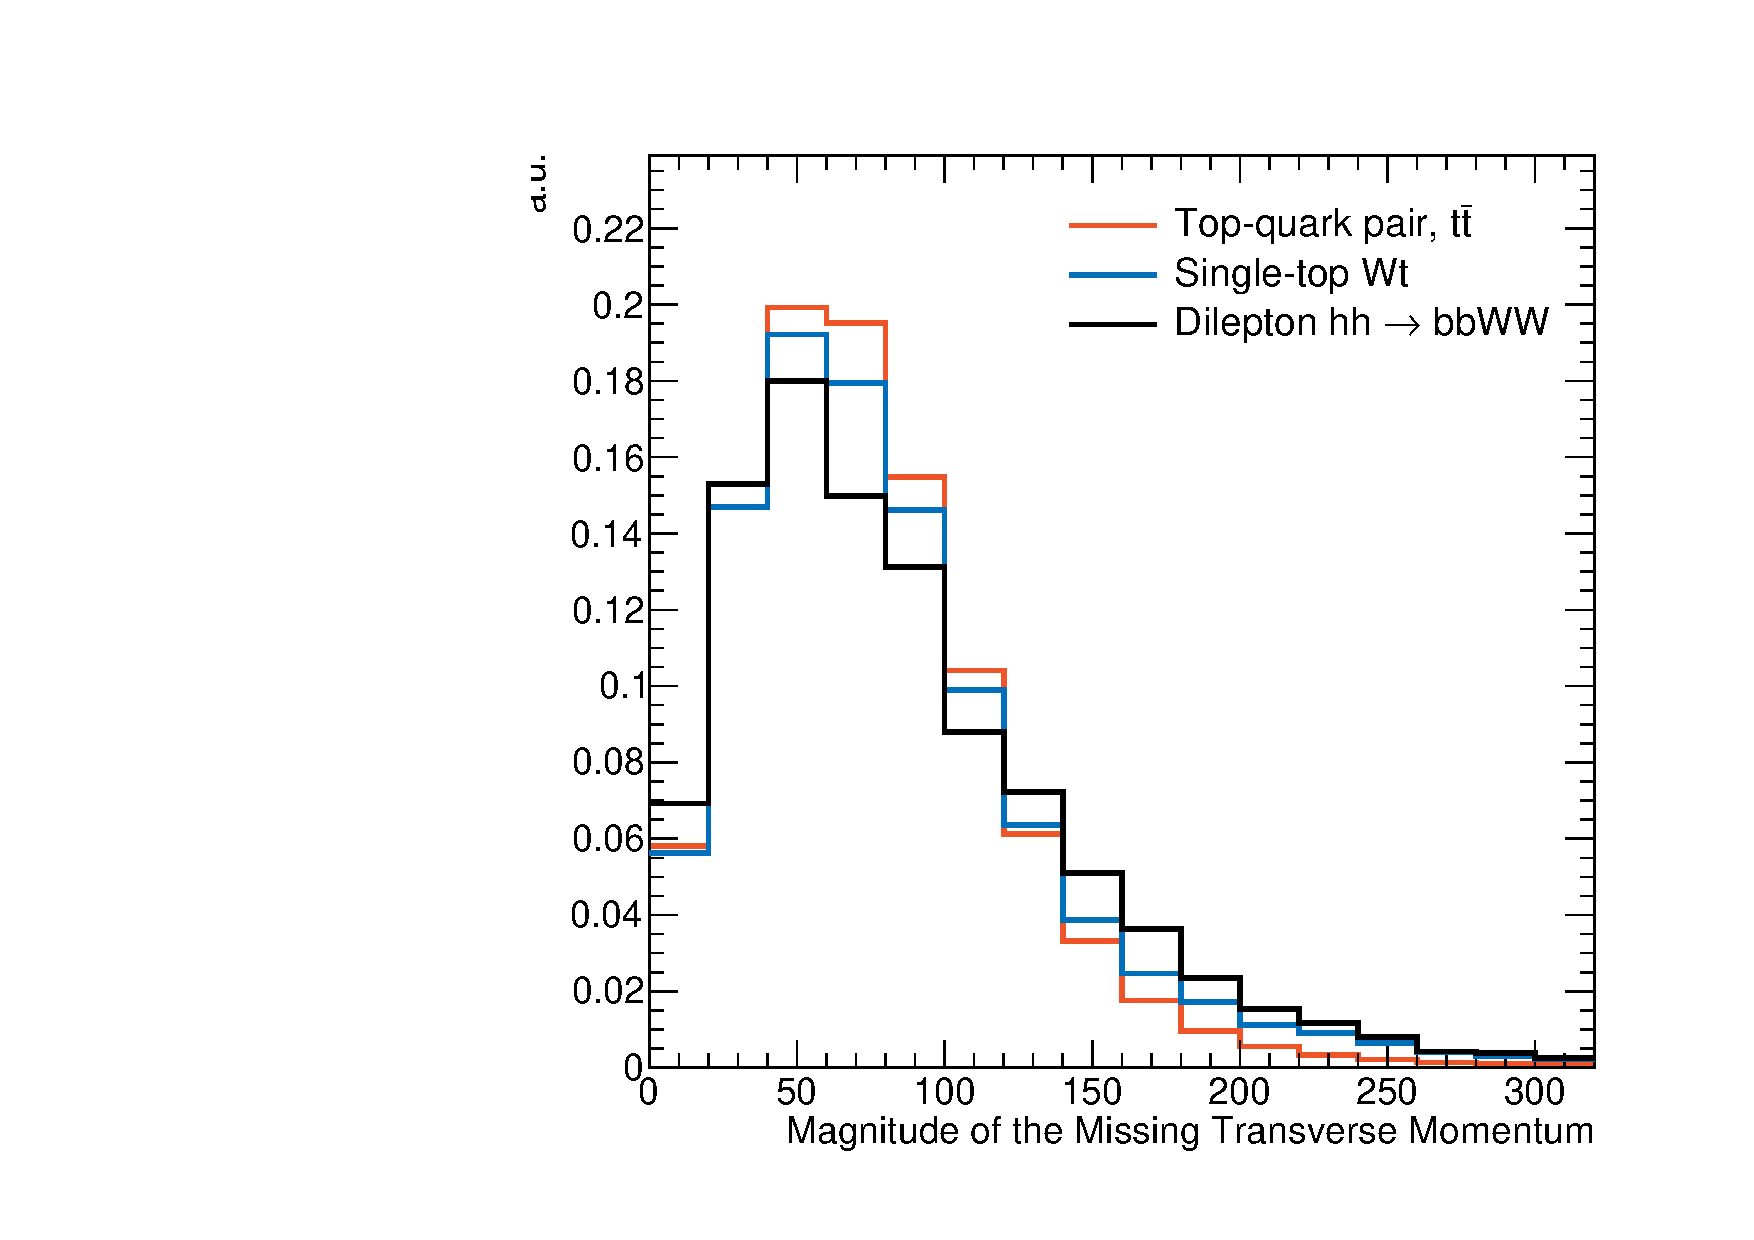
\includegraphics[width=0.45\textwidth]{figures/search_hh/signal_pheno/shape_plots/hh_shape_plot_met}
        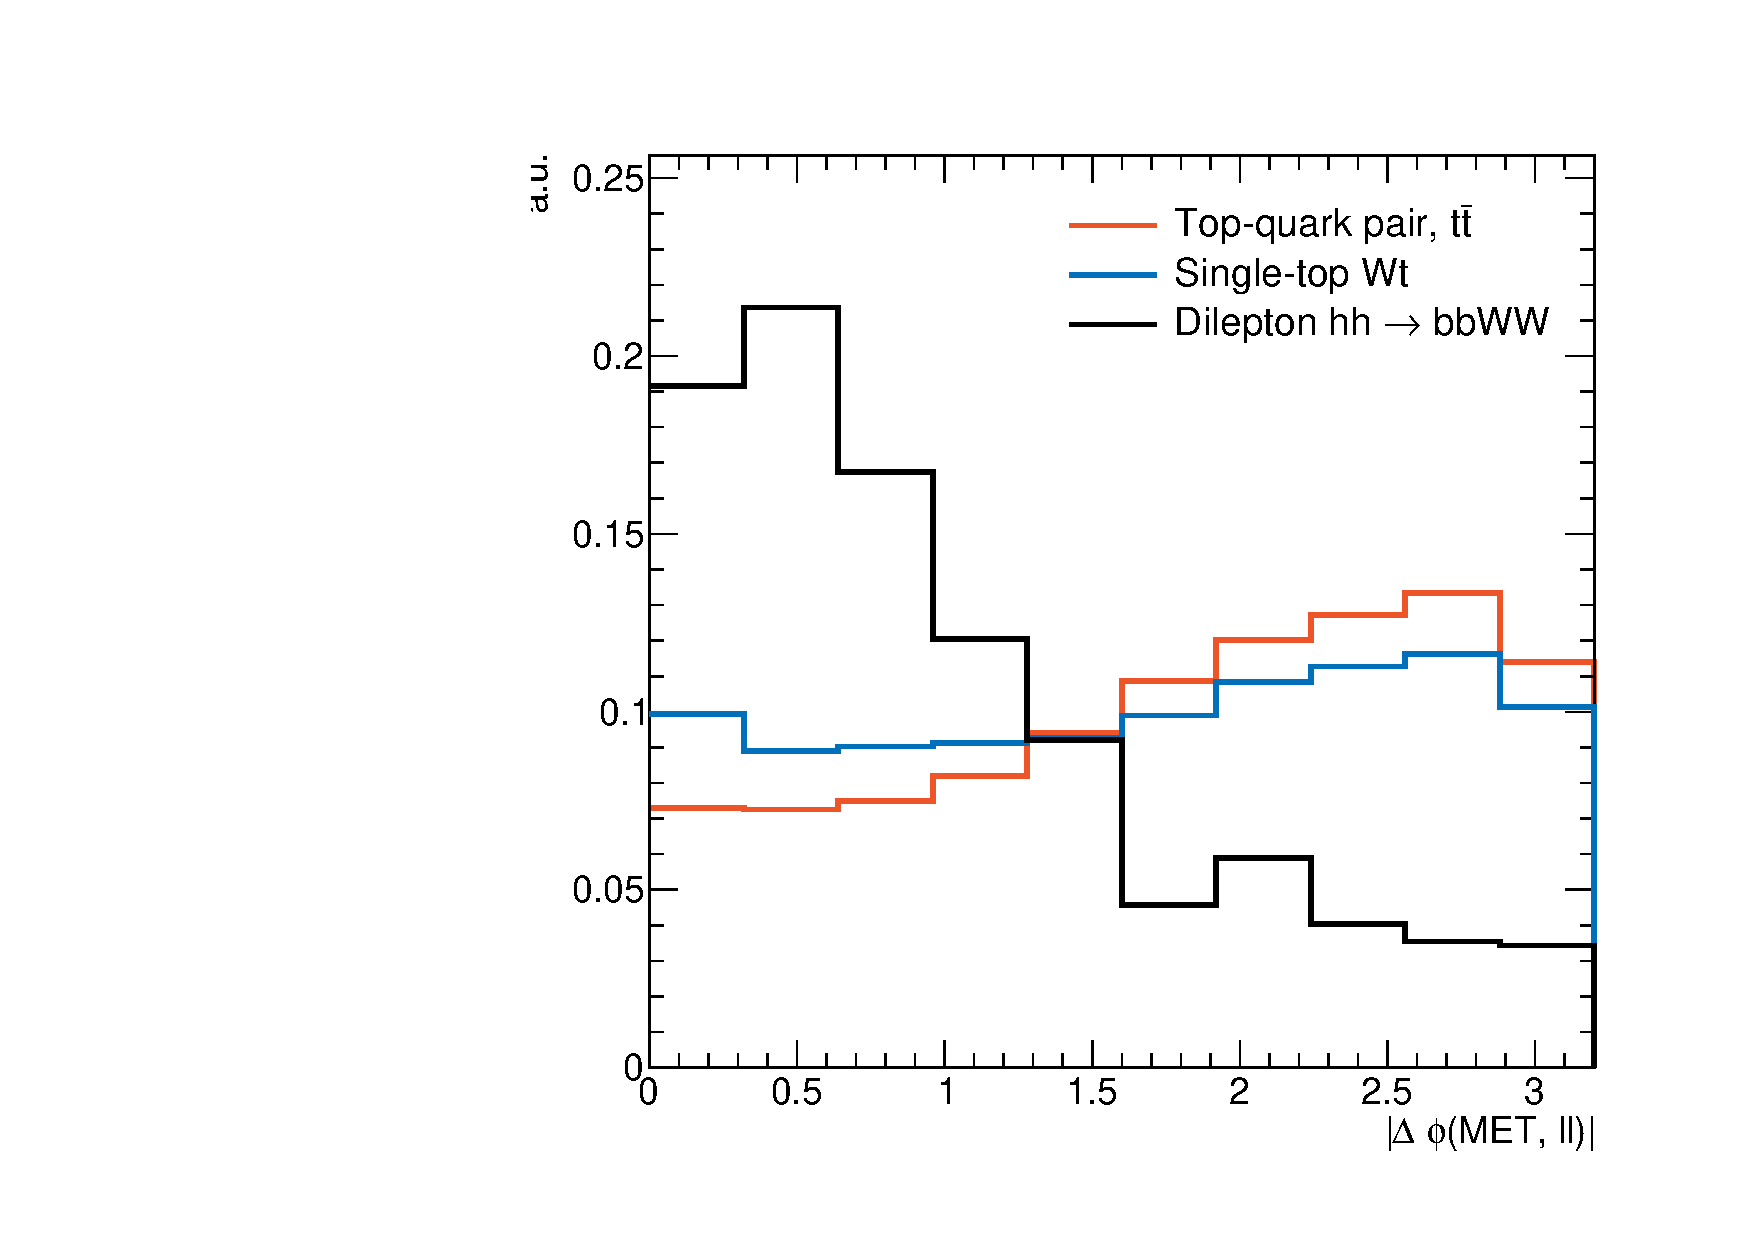
\includegraphics[width=0.45\textwidth]{figures/search_hh/signal_pheno/shape_plots/hh_shape_plot_dphi_met_ll}
        \caption{
            Normalized distributions showing the shapes of kinematic distributions for the SM
            top-quark processes (\ttbar~and single-top $Wt$) and the dilepton $hh \rightarrow \bbww$ signal process.
            \textit{\textbf{Left, upper}}: $|\Delta \phi|$ between the two leptons, $|\dphill|$.
            \textit{\textbf{Right, upper}}: $\Delta R$ between the two leptons, $\drll$.
            \textit{\textbf{Left, lower}}: Magnitude of the missing transverse momentum, \met.
            \textit{\textbf{Right, lower}}: $\Delta \phi$ between \met and dilepton system, $|\dphimetll|$.
        }
        \label{fig:hh_kin_1}
    \end{center}
\end{figure}

%%%%%%%%%%%%%%%%%%%%%%%%%%%%%%%%%%%%%%%%%%%%%%%%%%%%%%%%%%%%%%%%%%%%%%%%%%%%%%%%%%%
%%%%%%%%%%%%%%%%%%%%%%%%%%%%%%%%%%%%%%%%%%%%%%%%%%%%%%%%%%%%%%%%%%%%%%%%%%%%%%%%%%%
%%%%%%%%%%%%%%%%%%%%%%%%%%%%%%%%%%%%%%%%%%%%%%%%%%%%%%%%%%%%%%%%%%%%%%%%%%%%%%%%%%%
%
% TARGETTED OBSERVABLES
%
%%%%%%%%%%%%%%%%%%%%%%%%%%%%%%%%%%%%%%%%%%%%%%%%%%%%%%%%%%%%%%%%%%%%%%%%%%%%%%%%%%%
%%%%%%%%%%%%%%%%%%%%%%%%%%%%%%%%%%%%%%%%%%%%%%%%%%%%%%%%%%%%%%%%%%%%%%%%%%%%%%%%%%%
%%%%%%%%%%%%%%%%%%%%%%%%%%%%%%%%%%%%%%%%%%%%%%%%%%%%%%%%%%%%%%%%%%%%%%%%%%%%%%%%%%%

To take further advantage of the topological differences mentioned in the preceding, we can construct
an observable that is sensitive to the overall distribution of the momentum flow in the event.
This is to capture the more `planar' nature of the dilepton $hh \rightarrow \bbww$ decay as compared
to that of the SM top-quark backgrounds.
This observable, \htratio, is defined as follows,
\begin{align}
    \htratio &= \frac{\htnum}{\htden},
    \label{eq:ht2ratio_def}
\end{align}
where the $\bm{p}_{\text{T}}^{\ell(b),0 \{1\}}$ are the transverse momenta of the leading \{subleading\} lepton ($b$-tagged jet).

The numerator of Equation~\ref{eq:ht2ratio_def} contains two parts, each the magnitude of a vectorial sum of transverse
momenta: the first part containing the objects associated with the $WW^*$ decay and the second with those associated
with the $bb$ decay.
For the dilepton $hh \rightarrow \bbww$ signal, then, the numerator is the sum of the magnitudes of each of the Higgs boson's
momenta.
The denominator appearing in Equation~\ref{eq:ht2ratio_def} is the scalar sum of the transverse momenta of each of the
final state objects considered in teh analysis.
By taking this ratio, a measure of the overall spread of the momentum in the event is obtained.

For the relevant SM top-quark processes, with the visible final state objects distributed more evenly
about the event, the quantities appearing in the numerator of Equation~\ref{eq:ht2ratio_def} will
tend to be smaller, due to vectorial cancellation, than in the case of the $hh$ signal.
Due to the Higgs hemispheres in the signal, with separately collinear $WW^*$ and $bb$ systems,
the numerator in Equation~\ref{eq:ht2ratio_def} will be large.
It follows, then, that the quantity \htratio should tend towards unity for the dilepton $hh \rightarrow \bbww$
signal process and towards lower values for the SM top-quark processes.
This behavior is illustrated in Figure~\ref{fig:hh_shape_htratio}.

\begin{figure}[!htb]
    \begin{center}
        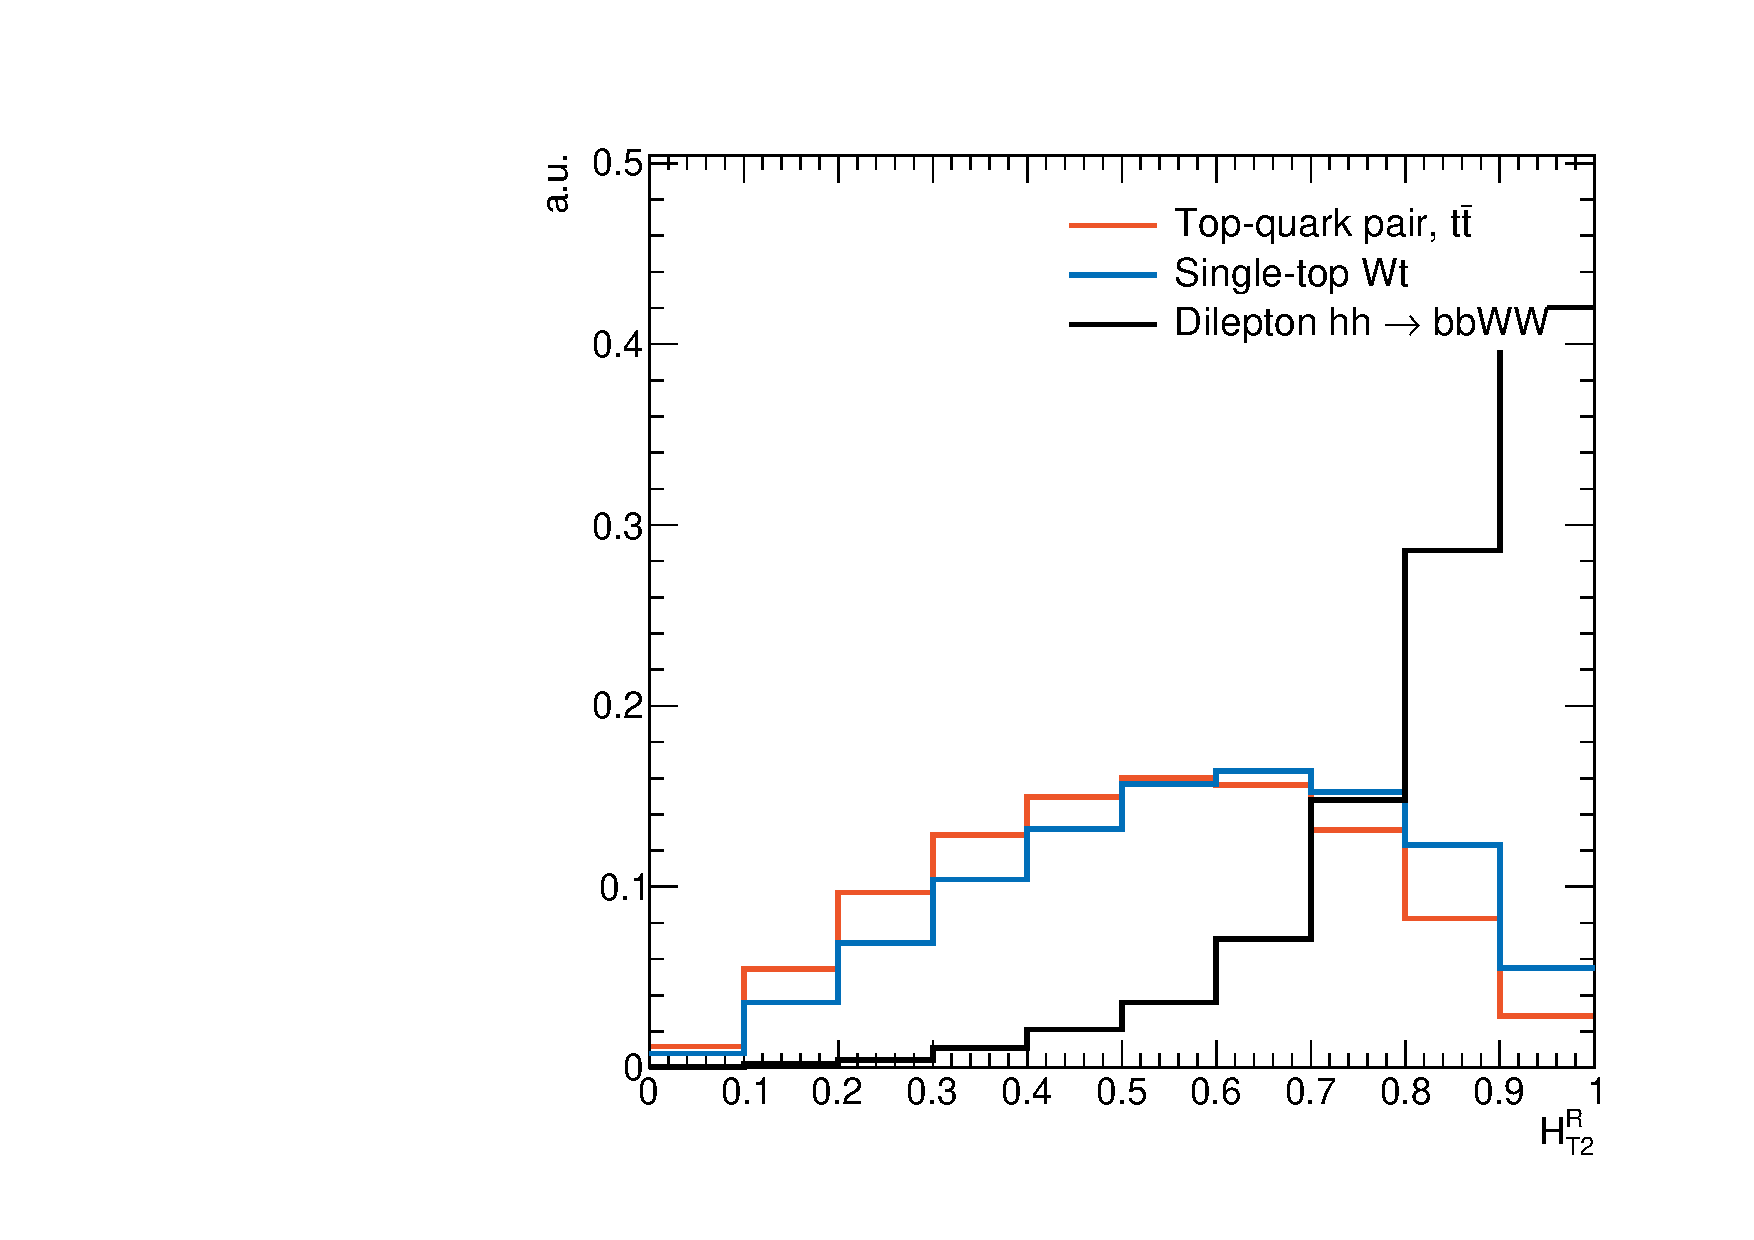
\includegraphics[width=0.6\textwidth]{figures/search_hh/signal_pheno/shape_plots/hh_shape_plot_HT2Ratio}
        \caption{
            Normalized distributions showing the shape of the \htratio observable for the SM
            top-quark processes (\ttbar~and single-top $Wt$) and the dilepton $hh \rightarrow \bbww$ signal process.
        }
        \label{fig:hh_shape_htratio}
    \end{center}
\end{figure}

We also consider a variant of the \mttwo variable~\cite{MT2-Glamour,Lester2011,MT2-Tovey-Masses,Lester2014yga},
a transverse-mass variable that can be used in events where there are two or more invisible particles,
as is our case with the two neutrinos.
Generally, \mttwo assumes that the decay is symemtric, as in \ttbar, where there are two decay legs, each with
a visible and invisible child particle decay.
The \mttwo observable is generically defined as follows,
\begin{align}
    \mttwo^2 \equiv \min\limits_{ \bm{q}_{\text{T}}^{\text{miss},\,a} + \, \bm{q}_{\text{T}}^{\text{miss},\,b} = \,\bm{p}_{\text{T}}^{\text{miss}}}
        \left[
            \max
                \left\{
                    m_{\text{T}}^2 ( \bm{p}_{\text{T}}^{\text{vis},\, a}, \bm{q}_{\text{T}}^{\text{miss},\,a} ), m_{\text{T}}^2 (\bm{p}_{\text{T}}^{\text{vis},\, b}, \bm{q}_{\text{T}}^{\text{miss},\,b} )
                \right\}
        \right],
    \label{eq:mttwo_def}
\end{align}
where `a' (`b') indicate one of the two sides of the decay and the $\bm{p}_{\text{T}}^i$ are the transverse momenta
of the visible objects on side $i \in (a,b)$, and $\bm{q}_{\text{T}}^i$ is a partition of the total \ptmiss given to side $i \in (a,b)$.
The minimization is carried out over all partionings of the \ptmiss into the $\bm{q}_{\text{T}}^i$ and the $m_{\text{T}}$ are the typical
transverse masses,
\begin{align}
    m_{\text{T}}^2 (\bm{p}_{\text{T}}^{\text{vis}}, \bm{q}_{\text{T}}^{\text{miss}} ) = ( E_{\text{T}}^{\text{vis}} + | \bm{q}_{\text{T}}^{\text{miss}} |)^2
            - |\bm{p}_{\text{T}}^{\text{vis}} + \bm{q}_{\text{T}}^{\text{miss}} |^2
    \label{eq:mt_def}
\end{align}

The \mttwo-based observable defined for the present analysis is referred to as `\mtbb',
and is an \mttwo construction in which the visible objects are the two $b$-tagged jets in the event.
This means that side `a' (`b'), using the notation of Equation~\ref{eq:mttwo_def}, contains
one of the $b$-tagged jets as $\bm{p}_{\text{T}}^{\text{vis, a}}$ ($\bm{p}_{\text{T}}^{\text{vis}, b}$).

Given the fact that in the SM top-quark backgrounds, the neutrinos (approximated by the $\bm{q}_{\text{T}}^{\text{miss}, i}$)
and the $b$-tagged jets originate from the same origin (a top-quark), the \mtbb observable tends
to have a kinematic bound at roughly the mass of the top-quark, $m_{\text{top}}$.
In the SM \ttbar~process, where both $b$-tagged jets originate from the decay of a top-quark, this kinematic
endpoint is strict.
In the case of single-top $Wt$, however, where only one $b$-tagged jet arises from the decay of a
top-quark, the kinematic endpoint at $m_{\text{top}}$ is not so strict and the \mtbb observable can extend beyond $m_{\text{top}}$.
Figure~\ref{fig:hh_shape_mtbb} illustrates the \mtbb observable.

\begin{figure}[!htb]
    \begin{center}
        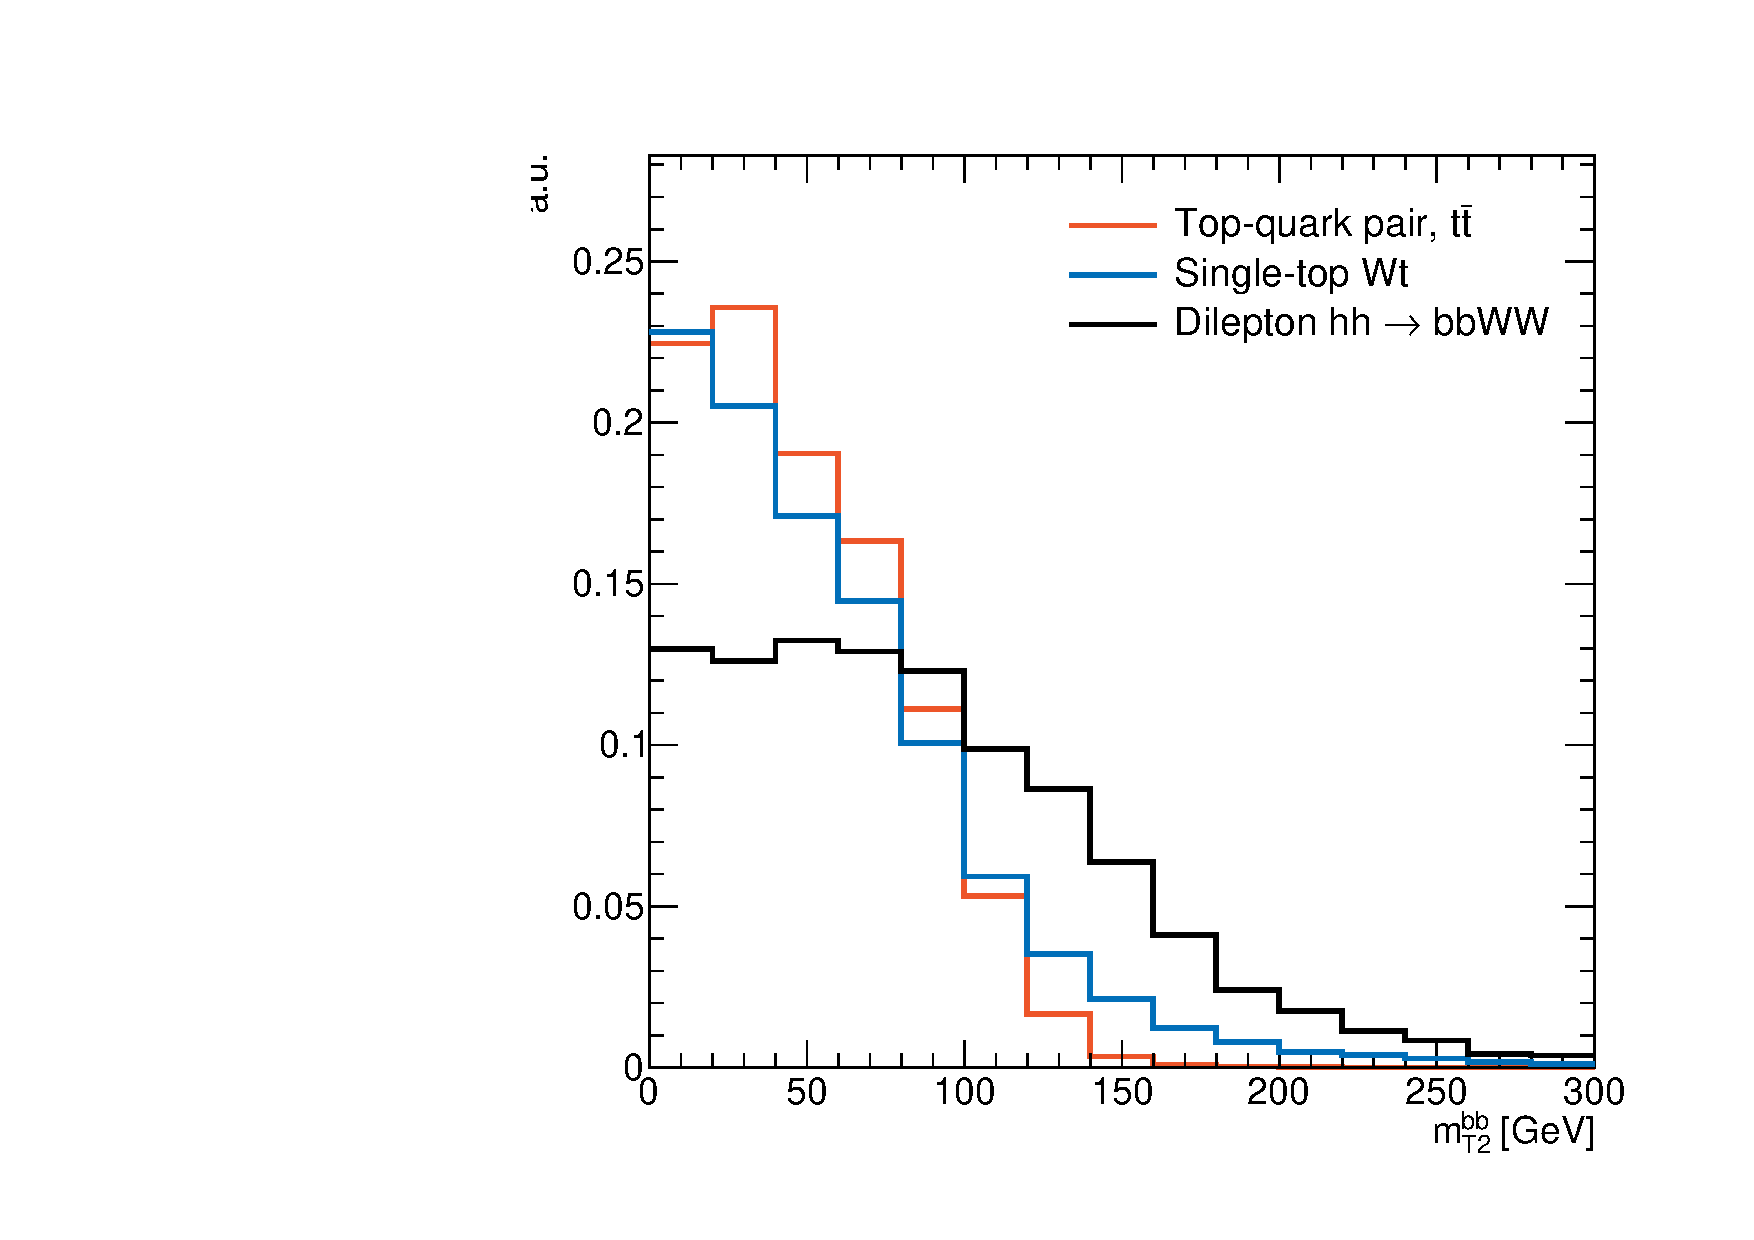
\includegraphics[width=0.6\textwidth]{figures/search_hh/signal_pheno/shape_plots/hh_shape_plot_mt2_bb}
        \caption{
            Normalized distributions showing the shape of the \mtbb observable for the SM
            top-quark processes (\ttbar~and single-top $Wt$) and the dilepton $hh \rightarrow \bbww$ signal process.
        }
        \label{fig:hh_shape_mtbb}
    \end{center}
\end{figure}



\section{Event Selection and Object Definitions}
\label{sec:hh_event_selection}

\section{Signal Selection}
\label{sec:stop_strategy}

%%%%%%%%%%%%%%%%%%%%%%%%%%%%%%%%%%%%%%%%%%%%%%%%%%%%%%%%%%%%%%%%%%%%%%%%%%%
%%%%%%%%%%%%%%%%%%%%%%%%%%%%%%%%%%%%%%%%%%%%%%%%%%%%%%%%%%%%%%%%%%%%%%%%%%%
%%%%%%%%%%%%%%%%%%%%%%%%%%%%%%%%%%%%%%%%%%%%%%%%%%%%%%%%%%%%%%%%%%%%%%%%%%%
%
% RJR
%
%%%%%%%%%%%%%%%%%%%%%%%%%%%%%%%%%%%%%%%%%%%%%%%%%%%%%%%%%%%%%%%%%%%%%%%%%%%
%%%%%%%%%%%%%%%%%%%%%%%%%%%%%%%%%%%%%%%%%%%%%%%%%%%%%%%%%%%%%%%%%%%%%%%%%%%
%%%%%%%%%%%%%%%%%%%%%%%%%%%%%%%%%%%%%%%%%%%%%%%%%%%%%%%%%%%%%%%%%%%%%%%%%%%
\subsection{The Recursive Jigsaw Reconstruction}
\label{sec:stop_rjr}

The \stopone search presented here makes use of of a high-level event reconstruction
technique referred to as the `Recursive Jigsaw Reconstruction' (RJR) technique~\cite{RecursiveJigsaw}.
This technique is a generalisation of the methods introduced in Ref.~\cite{SuperRazor}, referred
to as the `Super Razor'.

The RJR technique takes the measured information in an event --- the observable objects and their
four momenta, as well as the missing transverse momentum --- and, through a series of assumptions
and algorithms is able to reorganize those objects in such a way as to be interpreted as `fitting' into
a user-specified, or rather user-\textit{imposed}, decay tree.
Indeed, the technique's name derives from the methods it employs to perform this reorganization.
The `recursion' implied in the technique's name refers to the way in which its rules and algorithms
are implemented in order to \textit{navigate} through the decay tree: stepping through the decay
tree one level at at time, using information only from the current reference frame associated with
the object in the decay tree in that level, to determine the properties of the subsequent ones.
This effectively means that conclusions drawn at the `upper levels' of the decay about the kinematic
properties of the particles present are not lost or altered as one traverses further down the decay chain.
The `jigsaw' in the technique's name refers to the sets of rules and/or algorithms that are applied ---
so-called `Jigsaw Rules' --- in order to either piece together or break apart the reconstructed
event provided the kinematic information (lab-frame four-vectors) that the user has provided as input
to the decay tree assumption.

As an illustrative example of this decay tree `fitting', consider the \ttbar~and $\stopone \rightarrow b \chinoonepm$
decays illustrated in Figure~\ref{fig:rjr_ttbar_bcn}, which provides an example of an RJR decay tree imposition.
As will be outlined later, the RJR technique determines the relative velocities (boosts) between
the different states or rest-frames present in a given RJR decay tree.
These boosts between frames are illustrated diagrammatically as the black lines in the lower portion of
Figure~\ref{fig:rjr_ttbar_bcn} connecting the various states, both intermediate (`Decay States')
and final (`Visible States' or `Invisible States'), which are represented as the circles.
Although the two processes differ, they both fit topologically the RJR decay tree in Figure~\ref{fig:rjr_ttbar_bcn}.
In both cases, the final state is composed of two $b$-tagged jets, two leptons, and missing transverse
momentum and one can intuitively see how to allocate these objects' four-momenta to the states in the
RJR decay tree: the $V_{1\,(a,b)}$ states
are the $b$-tagged jets, the $V_{2\,(a,b)}$ states are the leptons, and the $I_{a,b}$ represent
the neutrinos (plus the LSPs in the case of the $\stopone \rightarrow b \chinoonepm$ signal).
Although the two processes may fit the same RJR tree, they are of course quite different kinematically
(e.g. the $I_{a,b}$ states for $\stopone \rightarrow b \chinoonepm$ are composed of additional
\textit{massive} particles in addition to the neutrinos) and any variable derived using the four-vectors
derived from this decay tree imposition has the potential to tease out these differences
between the signal and background processes.

\begin{figure}[!htb]
    \begin{center}
        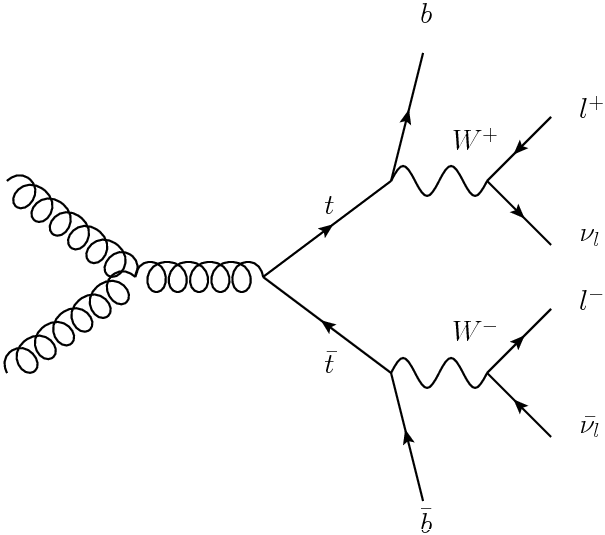
\includegraphics[width=0.4\textwidth]{figures/search_stop2l/strategy/fgraph_ttbar}
        \includegraphics[width=0.4\textwidth]{figures/search_stop2l/strategy/fgraph_stop_bCN}
        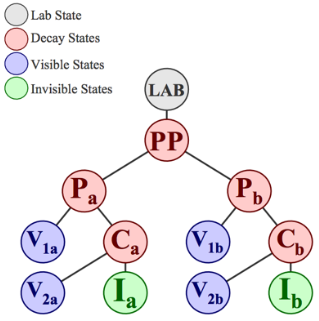
\includegraphics[width=0.5\textwidth]{figures/search_stop2l/strategy/RJRtree_generic_PPviaC}
        \caption{
            An example of an RJR decay tree interpretation of physics processes.
            The RJR decay tree (\textit{\textbf{bottom}}) can be fit to both the \ttbar~decay
            (\textit{\textbf{upper left}}) or the $\stopone \rightarrow b \chinoonepm$ process (\textit{\textbf{upper right}}).
            Each of the upper processes \textit{topologically} matches that of the RJR decay tree, but
            the underlying differences in their kinematics means that kinematic observables derived
            from this RJR decay tree may provide means of discrimination between the two.
            Each circle in the RJR decay tree represents a reconstructed reference frame,
            characterised by its own four-vector information.
        }
        \label{fig:rjr_ttbar_bcn}
    \end{center}
\end{figure}

\FloatBarrier
%%%%%%%%%%%%%%%%%%%%%%%%%%%%%%%%%%%%%%%%%%%%%%%%%%%%%%%%%%%%%%%%%%%%%%%%%%%
%%%%%%%%%%%%%%%%%%%%%%%%%%%%%%%%%%%%%%%%%%%%%%%%%%%%%%%%%%%%%%%%%%%%%%%%%%%
%%%%%%%%%%%%%%%%%%%%%%%%%%%%%%%%%%%%%%%%%%%%%%%%%%%%%%%%%%%%%%%%%%%%%%%%%%%
%
% RJR FOR THREE BODY
%
%%%%%%%%%%%%%%%%%%%%%%%%%%%%%%%%%%%%%%%%%%%%%%%%%%%%%%%%%%%%%%%%%%%%%%%%%%%
%%%%%%%%%%%%%%%%%%%%%%%%%%%%%%%%%%%%%%%%%%%%%%%%%%%%%%%%%%%%%%%%%%%%%%%%%%%
%%%%%%%%%%%%%%%%%%%%%%%%%%%%%%%%%%%%%%%%%%%%%%%%%%%%%%%%%%%%%%%%%%%%%%%%%%%

The RJR decay tree imposed in the present analysis searching for the three-body decay
of the \stopone quark is presented in Figure~\ref{fig:rjr_stop}.
The visible system ($V_a + V_b$) is provided only the two leptons in the event.
The invisible system ($I_a + I_b$) is provided the missing transverse momentum.

\begin{figure}[!htb]
    \begin{center}
        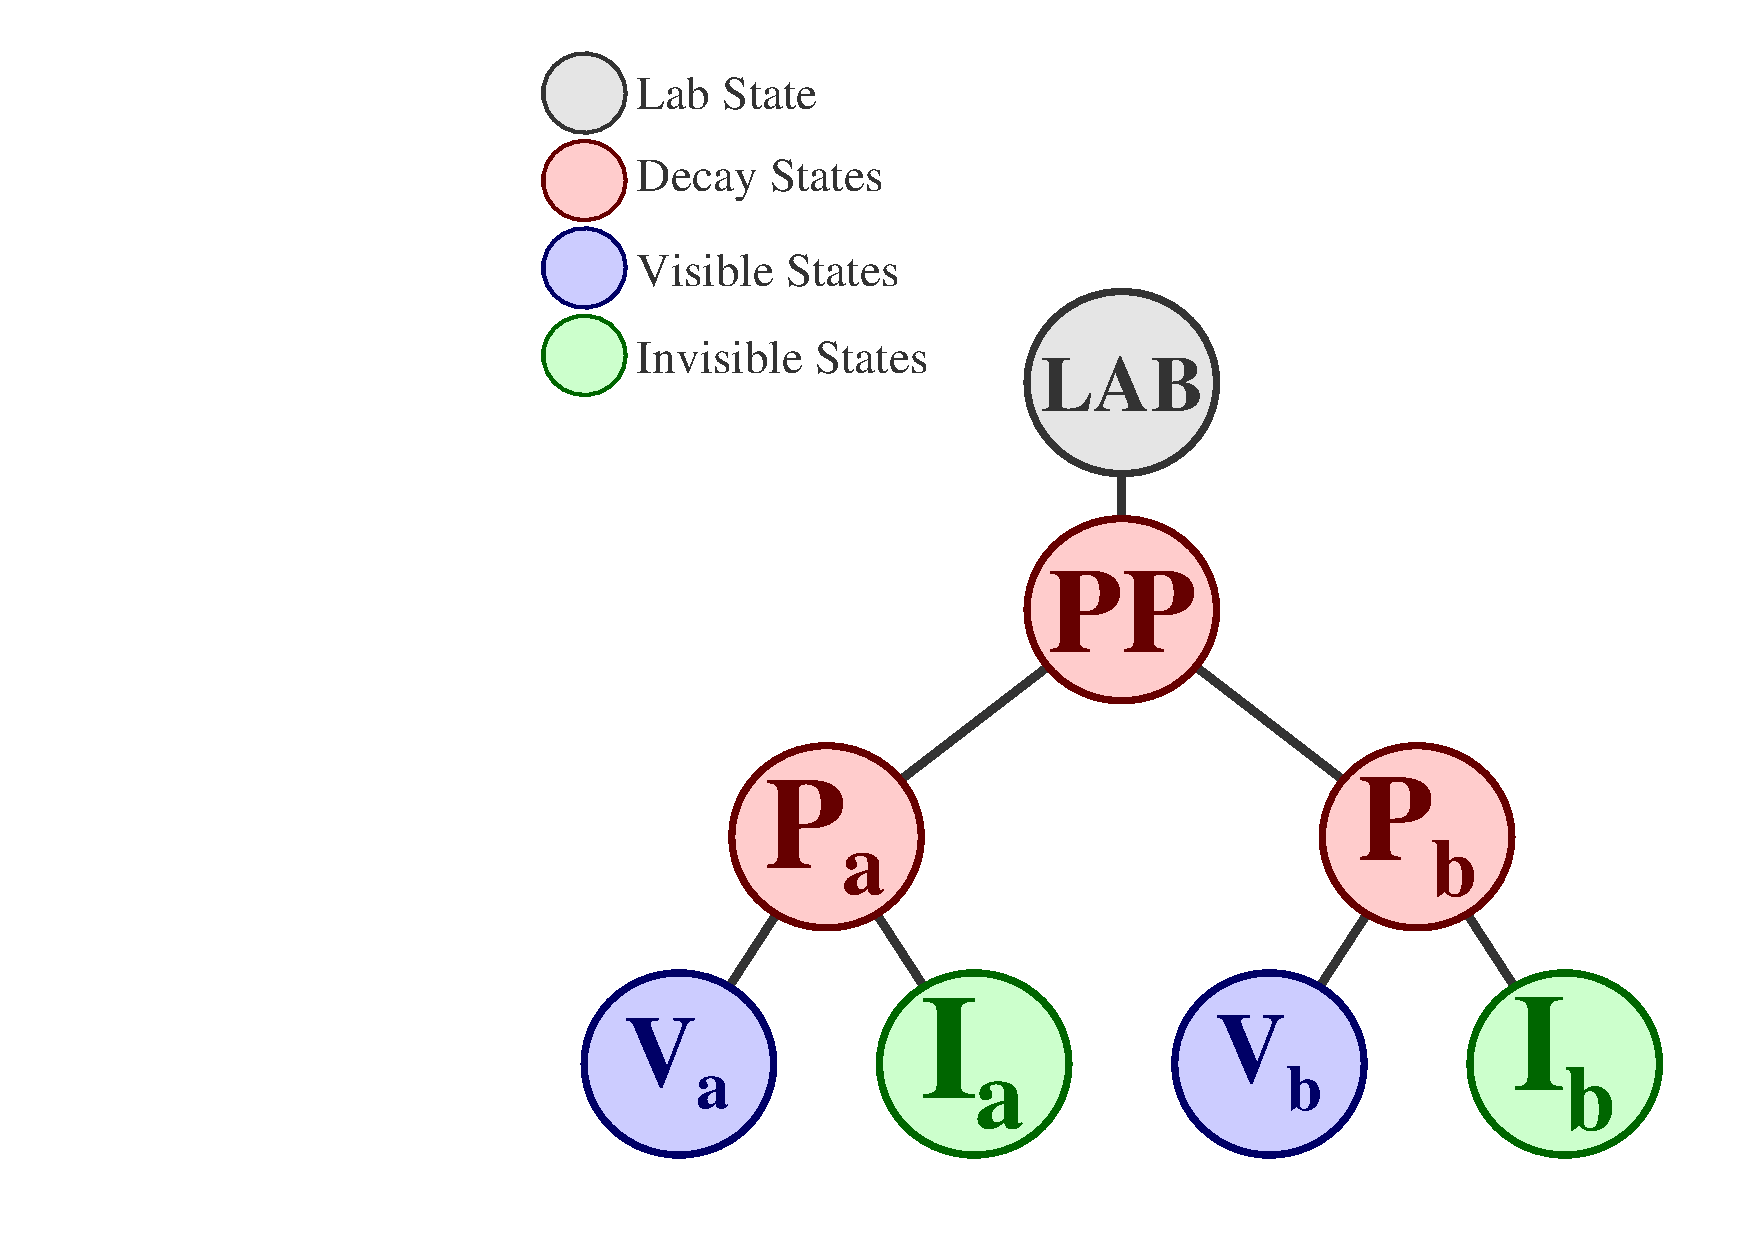
\includegraphics[width=0.6\textwidth]{figures/search_stop2l/strategy/RJRtree_DiSparticle}
        \caption{
            RJR decay tree assumption used in the 2015+2016 analysis searching for the
            three-body decay of the \stopone quark, $\stopone \rightarrow b W \ninoone$.
            It is the most general decay tree for $R$-parity conserving SUSY scenarios in
            which pair-produced sparticles ($P_a$ and $P_b$) each decay to visible states ($V_a$ and $V_b$)
            and invisible states ($I_a$ and $I_b$).
            Each of the final states ($V_i$ and/or $I_i$) may, in principle, be composed of multiple particles.
            In the present analysis, only the two leptons in the event are provided as inputs to the $V_i$ and both
            are required to be non-empty (i.e. $V_a$ is one of the leptons, $V_b$ the other).
            The missing transverse momentum in the event is decomposed via a set of Jigsaw Rules into the
            states $I_a$ and $I_b$.
        }
        \label{fig:rjr_stop}
    \end{center}
\end{figure}

The RJR decay tree in Figure~\ref{fig:rjr_stop} is the most general RJR decay tree one can make for
targeting $R$-parity conserving SUSY models.
This decay tree makes the least number of assumptions on the decay of the pair-produced sparticles and
their children (if any).
This is beneficial, as developing a search (whose a-priori intent is for discovery of new physics)
that is largely dependent on the model assumed for designing the analysis' selection criteria
greatly limits the applicability and scope of that search.
For example, one can imagine using the decay tree of Figure~\ref{fig:rjr_ttbar_bcn} also for the three-body
decays considered in the present search, $\stopone \rightarrow b W \ninoone$.
However, the decay tree in Figure~\ref{fig:rjr_ttbar_bcn} assumes that there is enough information to
kinematically separate the $b$-tagged jets and leptons into the $V_{1(a,b)}$ and $V_{2(a,b)}$ states,
respectively, therefore requiring at least four visible objects to be reconstructed.
As discussed in Section~\ref{sec:stop_final_state}, this is not the case for the three-body decays
of the \stopone relevant for the present analysis and so Figure~\ref{fig:rjr_ttbar_bcn} is not well-suited
for this search.
What we want, in the end, is a means to separate from the background the presence of an $R$-parity conserving
SUSY signal while making as few assumptions as possible.

As mentioned, the goal of the RJR technique is to provide a full accounting of all of the states specified by the
user in the imposed RJR decay tree; or, at least a close and/or optimal approximation of them.
Unfortunately, it is in general impossible to do this as a result of the presence of multiple weakly interacting
particles in the final state and, less generally, because of combinatoric ambiguities
that make it difficult to assign objects to specific locations in the decay (e.g. associating $b$-jets to
the correct side of the decay).
The RJR technique and its so-called Jigsaw Rules provide a means to systematically resolve these unknowns
on an event-by-event basis.

In order to resolve combinatoric ambiguities amongst the reconstructed visible objects so that they may
be grouped `correctly', one can employ a Jigsaw Rule for performing a recursive partitioning
of the visible objects until that grouping which minimizes the visible mass of each side of a decay vertex is found.
This is not necessarily the true grouping, but it is a method that is found to reproduce well, on average,
the correct grouping of objects.

In the RJR decay tree used in the search for $\stopone \rightarrow b W \ninoone$, illustrated
in Figure~\ref{fig:rjr_stop}, there are 6 under-constrained degrees-of-freedom (DOF) due to the
weakly interacting particles/missing transverse momentum.
These are (2 DOF for each) as follows:
\begin{itemize}
    \item The longitudinal momenta of the $I_i$ states: $p_{I_i,z}$
    \item The splitting of the missing transverse momentum between the $I_i$ states: $\bm{p}_{I_a,T} + \bm{p}_{I_b,T} = \bm{E}_T^{\text{miss}}$
    \item The mass of the di-invisible system composed of $I_a$ and $I_b$: $m_I$ ($m_{I_a}$ and $m_{I_b}$)
\end{itemize}
The RJR technique sets out to provide values for these unknowns through assumptions (constraints) that it makes
for determining the relative velocities (boosts) between rest-frames indicated by the circles in Figure~\ref{fig:rjr_stop}.
The recursive element of the technique is most obvious in this respect: the algorithm moves from
the first known reference frame (the lab frame) and traverses down the decay tree using information
only from the current frame to determine the boosts for moving into the next reference frame.
That is, with respect to Figure~\ref{fig:rjr_stop}, information only from the lab frame
is used to move to the $PP$ (center-of-mass, COM) frame and information from this COM frame
is used to move to either of the respective $P_i$ frames.
There are specific Jigsaw Rules at each step of this navigating of the RJR decay tree that determine
\textit{how} the information in each of these frames is used simultaneously to move to the next
and to provide estimates of the under-constrained DOF mentioned above.

The first step that the RJR technique takes in constructing the boosts relating the reference frames is to
determine the mass of the invisible system, $m_I$, composed of the states $I_a$ and $I_b$.
This information is required to be able to consistently perform boosts between the reference frames while
keeping each side, or \textit{hemisphere}, of the decay balanced against the other.
This means that, generally, the di-invisible system will have non-trivial opening angles between the $I_i$
states in order to balance the visible system frame-by-frame.
This means that it will attain a mass\footnote{From special relativistic mechanics, the mass of a system comprised
of two subsystems, 1 and 2, is generally given by $m_{12}^2 = m_1^2 + m_2^2 + 2(E_1E_2 - |\vec{p}_1| |\vec{p}_2| \cos \theta_{12})$,
where $\theta_{12}$ is the opening angle between $\vec{p}_1$ and $\vec{p}_2$.}
To satisfy this balancing requirement, the RJR technique takes for $m_I$ the smallest Lorentz-invariant
mass consistent with the input lab-frame observables that will accommodate the subsequent boosts and also prevent
the states $I_i$ from becoming tachyonic.
For the decay tree in Figure~\ref{fig:rjr_stop} this turns out to be,
\begin{align}
    m_I^2 = m_V^2 - 4m_{V_a} m_{V_b},
    \label{eq:rjr_invisible_mass}
\end{align}
where $V$ refers to the total visible system comprised of $V_a$ and $V_b$.

Next, the RJR technique determines the boost from the lab to the $PP$ (COM) frame.
To determine this boost, we must determine the longitudinal momentum of the invisible system, $p_{I,z}^{\text{Lab}}$,
which is one of the under-constrained DOF.
The RJR technique chooses this value such that the rapidity of the visible and invisible systems are equal.
This choice results in our choice of the $PP$ (COM) reference frame being a longitudinally boost-invariant
choice, meaning that all subsequent observables derived in the RJR decay tree will also be
longitudinally boost-invariant.
Additionally, one can see that this also forces the mass of the $PP$ system, $m_{V+I}$, to
take its minimum value.\footnote{This is seen using the previous footnote and knowledge that $\vec{E}_T^{\text{miss}}$
must balance the visible system's transverse momentum.}

With the longitudinal momentum of the invisible system determined, along with its mass, we have
the expression for the boost relating the lab frame to the $PP$ (COM) frame:
\begin{align}
    \vec{\beta}_{PP}^{\,\text{LAB}} = \frac{
        \vec{p}_{PP}^{\text{LAB}}
    }
    {
        E_{PP}^{\text{LAB}}
    }
    = \frac{
        \vec{p}_V^{\,\text{LAB}} + \vec{p}_I^{\,\text{LAB}}
    }
    {
        E_V^{\text{LAB}} + \sqrt{ |\vec{p}_I^{\,\text{LAB}} |^2 + m_I^2 }
    }.
    \label{eq:rjr_lab_boost}
\end{align}
The boost in Equation~\ref{eq:rjr_lab_boost} affords provides us the observables in the $PP$ (COM)
reference frame.
We must use information in this frame to determine how to move to the individual sparticle frames, $P_i$.
This will provide us with the last set of information regarding how the missing transverse momentum
is to be shared between the states $I_i$.
Here, the RJR technique makes the assumption that $m_{V_a} = m_{V_b}$, which, in the context of the processes
considered, is reasonable.
As we are in the COM frame, this choice for the masses of the $V_i$ states dictates that the boosts of each of their
individual reference frames be equal in magnitude and anti-parallel.
For our decay tree, a possible solution for this is chosen to be:
\begin{align}
    \vec{\beta}_{P_i}^{\,PP} = \frac{
        \vec{p}_{V_a}^{\,PP} - \vec{p}_{V_b}^{\,PP}
    }
    {
        E_{V_a}^{PP} + E_{V_b}^{PP}
    }.
    \label{eq:rjr_pi_boost}
\end{align}
Under this boost, all observables subsequently defined are \textit{contra-boost invariant}, meaning that,
as in the case for the longitudinal boost invariance described previously, all observables
are therefore insensitive (on average) to the fact that this boost from the $PP$ (COM) frame to the $P_i$
frames is not necessarily the true boost.
Indeed, this final contra-boost invariance is the main motivation behind the structure of Equation~\ref{eq:rjr_pi_boost}.

Now that we have the boost $\vec{\beta}_{P_i}^{\,PP}$ to the $P_i$ frames, one can determine the splitting of invisible
momentum by requiring $\vec{p}_{V_i}^{\,P_i} + \vec{p}_{I_i}^{\,P_i} = 0$, which
is the final under-constrained DOF of the RJR decay tree relevant to the analysis being presented.

With the application of the RJR technique, then, all of the unknowns in the event are thus determined
(approximately), and one has access to kinematic information (four vectors) for every level of the RJR decay tree
that has been imposed (Figure~\ref{fig:rjr_stop}).

\FloatBarrier
%%%%%%%%%%%%%%%%%%%%%%%%%%%%%%%%%%%%%%%%%%%%%%%%%%%%%%%%%%%%%%%%%%%%%%%%%%%
%%%%%%%%%%%%%%%%%%%%%%%%%%%%%%%%%%%%%%%%%%%%%%%%%%%%%%%%%%%%%%%%%%%%%%%%%%%
%%%%%%%%%%%%%%%%%%%%%%%%%%%%%%%%%%%%%%%%%%%%%%%%%%%%%%%%%%%%%%%%%%%%%%%%%%%
%
% DISCRIMINATING VARIABLES
%
%%%%%%%%%%%%%%%%%%%%%%%%%%%%%%%%%%%%%%%%%%%%%%%%%%%%%%%%%%%%%%%%%%%%%%%%%%%
%%%%%%%%%%%%%%%%%%%%%%%%%%%%%%%%%%%%%%%%%%%%%%%%%%%%%%%%%%%%%%%%%%%%%%%%%%%
%%%%%%%%%%%%%%%%%%%%%%%%%%%%%%%%%%%%%%%%%%%%%%%%%%%%%%%%%%%%%%%%%%%%%%%%%%%

\subsection{Discriminating Observables}
\label{sec:stop_variables}

In this section we describe the basis of kinematic observables, defined using the states defined
by the RJR, that are used to define the SRs, CRs, and VRs in the present analysis.

With the RJR technique providing us with an approximation of the center-of-mass frame of the
\stop system (the state $PP$ in Figure~\ref{fig:rjr_stop}), a natural variable to define is the
total energy, or invariant mass, available to those objects in our decay tree.
With the entire system defined, this can be obtained easily and we refer to this
approximate COM energy as $m_{PP}$, shown in Figure~\ref{fig:rjr_mpp}.

\begin{figure}[!htb]
    \begin{center}
        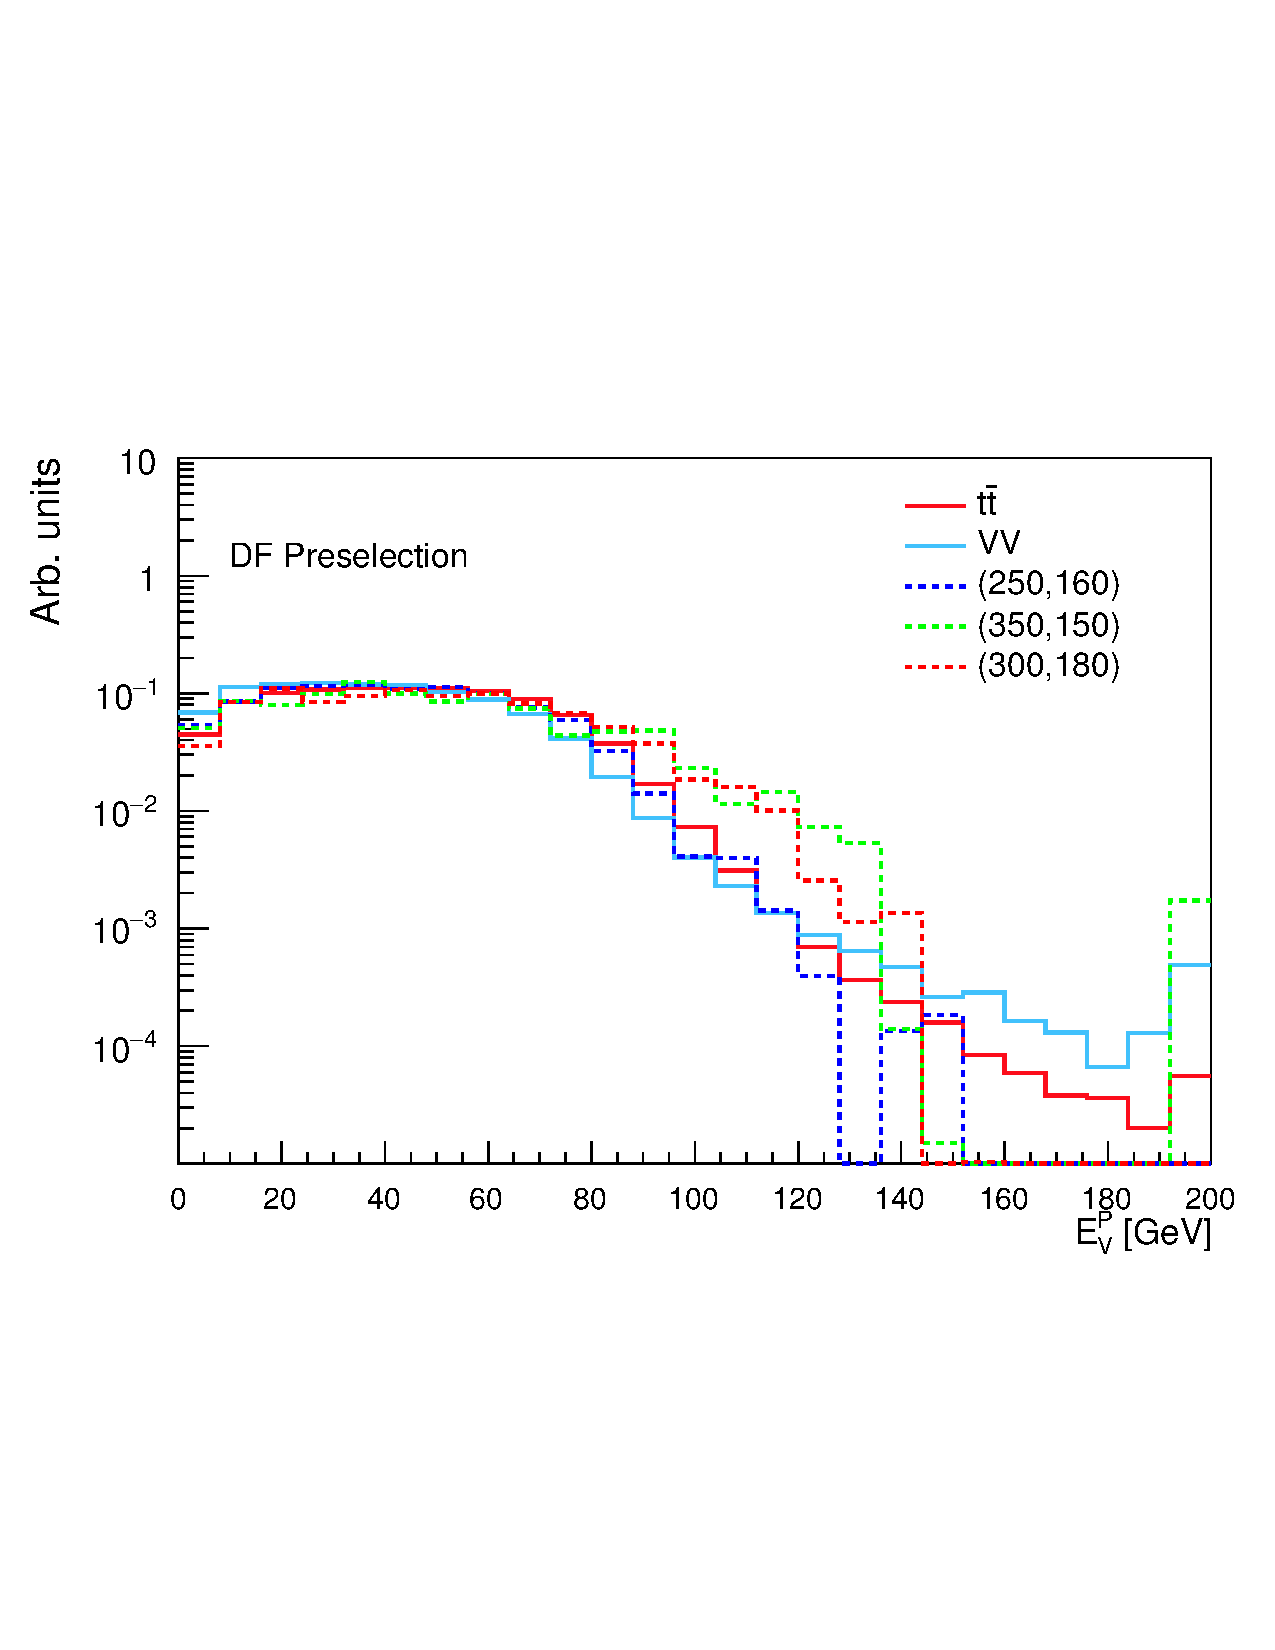
\includegraphics[width=0.7\textwidth]{figures/search_stop2l/strategy/comp_plots/dfpresel_MDR}
        \caption{
            Normalised distribution of the $m_{PP}$ variable for several $\stopone \rightarrow b W \ninoone$
            signal hypotheses, labeled with respect to their assumed $(m_{\stopone}, m_{\ninoone})$ values in the
            legend.
            The SM \ttbar~and diboson ($VV$) background processes are also shown for comparison.
        }
        \label{fig:rjr_mpp}
    \end{center}
\end{figure}

In addition to $m_{PP}$, we can define the associated transverse momentum of the COM frame,
$|\vec{p}_T^{\,PP}|$, shown in Figure~\ref{fig:rjr_pTT_T}.
Used in conjunction, the two variables $m_{PP}$ and $|\vec{p}_T^{\,PP}|$ can be used to build the
ratio, $R_{p_T}$, defined as:
\begin{align}
    R_{p_T}  = \frac{
        |\vec{p}_T^{\,PP}|
    }
    {
        |\vec{p}_T^{\,PP}| + m_{PP}/4
    }.
    \label{eq:rjr_rpt}
\end{align}
Distributions of $R_{p_T}$ are provided in Figure~\ref{fig:rjr_RPT}.
The more central nature of our signal hypothesis wherein the pair-produced sparticles decay to
heavy final state objects and distribute more of their energy to the transverse plane can be seen
in Figure~\ref{fig:rjr_RPT}.

\begin{figure}[!htb]
    \begin{center}
        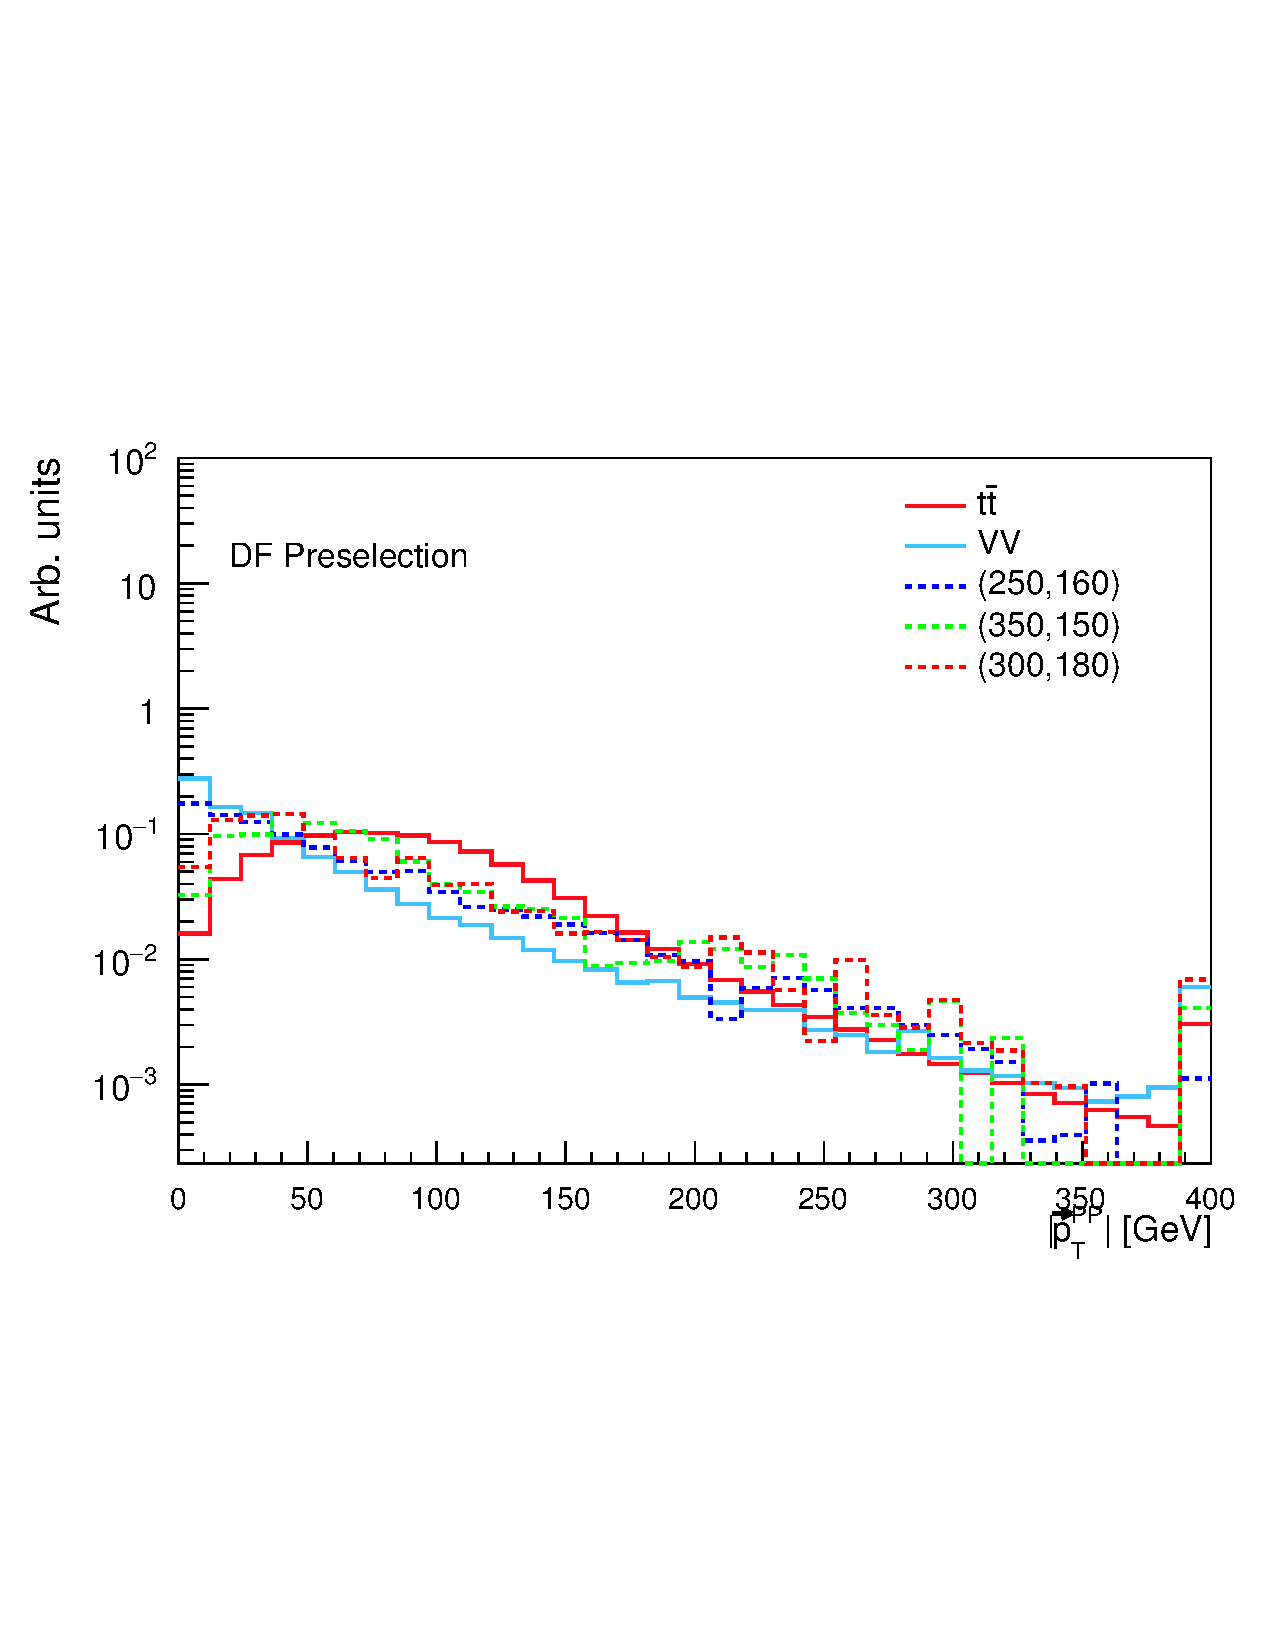
\includegraphics[width=0.7\textwidth]{figures/search_stop2l/strategy/comp_plots/dfpresel_pTT_T}
        \caption{
            Normalised distribution of the $|\vec{p}_T^{\,PP}|$ variable for several $\stopone \rightarrow b W \ninoone$
            signal hypotheses, labeled with respect to their assumed $(m_{\stopone}, m_{\ninoone})$ values in the
            legend.
            The SM \ttbar~and diboson ($VV$) background processes are also shown for comparison.
        }
        \label{fig:rjr_pTT_T}
    \end{center}
\end{figure}

\begin{figure}[!htb]
    \begin{center}
        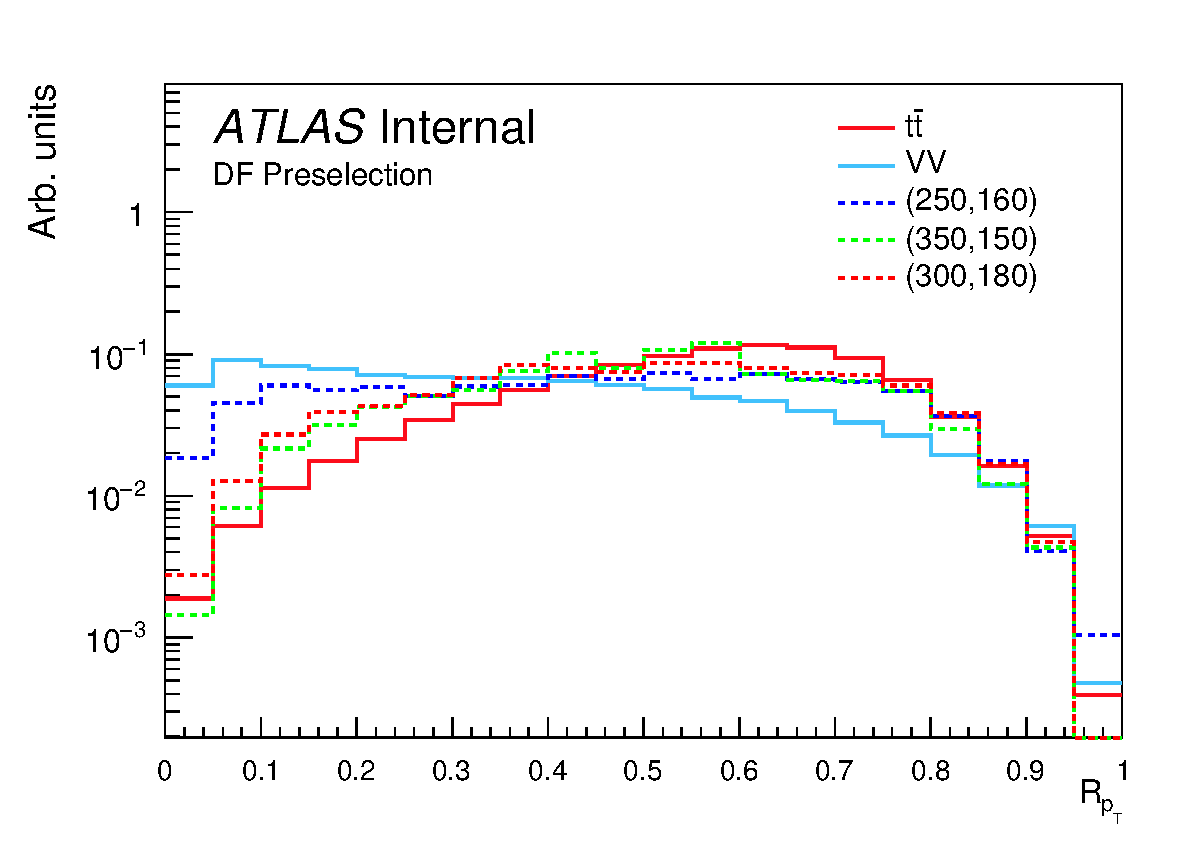
\includegraphics[width=0.7\textwidth]{figures/search_stop2l/strategy/comp_plots/dfpresel_RPT}
        \caption{
            Normalised distribution of the $R_{p_T}$ variable for several $\stopone \rightarrow b W \ninoone$
            signal hypotheses, labeled with respect to their assumed $(m_{\stopone}, m_{\ninoone})$ values in the
            legend.
            The SM \ttbar~and diboson ($VV$) background processes are also shown for comparison.
        }
        \label{fig:rjr_RPT}
    \end{center}
\end{figure}

The next variable that can be defined uses the relative velocity of the $PP$ frame as seen
in the LAB frame, as well as the total visible system $V = V_a + V_b$ as seen in the $PP$ frame.
This is the azimuthal angle between the velocity, or boost, from the LAB to $PP$ frame and the visible
system $V$ (which, in our case, is simply the dilepton system) as seen in the $PP$ (COM) frame.
This variable, \dpb, is shown in Figure~\ref{fig:rjr_DPB}.

The key features of the angular quantity \dpb can be seen in Figure~\ref{fig:rjr_DPB}.
The \stopone signals clearly peak more strongly near values of $\dpb \sim \pi$ and are roughly
overlapping for all values of $\sdiff$, meaning that the behavior of \dpb is loosely
independent on \sdiff.
Rather, \dpb tends to be more dependent on the assumptions gone into constructing the underlying
RJR decay tree in Figure~\ref{fig:rjr_stop}, from which the quantity \dpb is ultimately derived.
As discussed, with the dilepton system $V = V_a + V_b$, Equation~\ref{eq:rjr_invisible_mass} results
in the assumption $m_I = m_V$.
For the massive \ninoone particles in the invisible final state of our \stopone signal decays, this
assumption is clearly incorrect and means that the boost from the LAB frame to the approximate 
$PP$ (COM) frame tends to be an \textit{over}-boost since the assumption of equal masses assumes
too much momentum for the invisible system.
In reality, on the other hand, much of the \stopone energy-momentum goes
into the \textit{mass} of the invisible system.
This over-boosting can be seen in Equation~\ref{eq:rjr_lab_boost} with the under-predicted $m_I$
in the denominator.
This results in the system $V$ to point, on average, in the opposite (anti-parallel) direction with
respect to the boost in Equation~\ref{eq:rjr_lab_boost} when viewed in the approximate COM frame, $PP$.

\begin{figure}[!htb]
    \begin{center}
        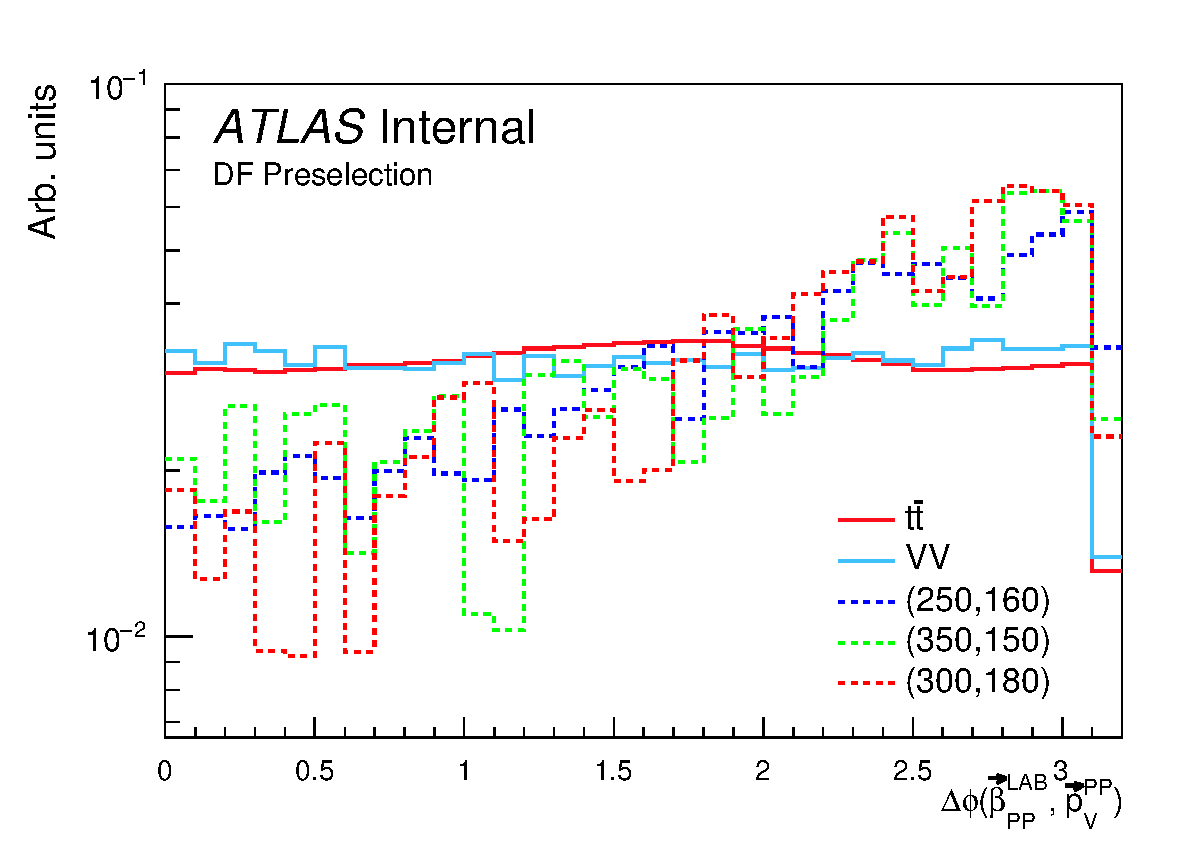
\includegraphics[width=0.7\textwidth]{figures/search_stop2l/strategy/comp_plots/dfpresel_DPB_vSS}
        \caption{
            Normalised distribution of the $\dpb$ variable for several $\stopone \rightarrow b W \ninoone$
            signal hypotheses, labeled with respect to their assumed $(m_{\stopone}, m_{\ninoone})$ values in the
            legend.
            The SM \ttbar~and diboson ($VV$) background processes are also shown for comparison.
        }
        \label{fig:rjr_DPB}
    \end{center}
\end{figure}

We can also define a variable that is sensitive to the (squared) mass differences between the pair-produced
\stopone and final state \ninoone.
This observable, corresponding to the energy of one of the $V_i$ (one of the leptons) with respect to the sparticle $P_i$ frames
of reference.
This variable, $E_V^P$, can be interpreted as the approximate energy of the state $V_i$ in the frame
corresponding to $P_i$ and has an endpoint following,
\begin{align}
    E_V^P \propto \frac{
        m_{P_i}^2 - m_{I_i}^2
    }
    {
        m_{P_i}
    },
    \label{eq:mdr_endpoint}
\end{align}
which follows essentially from special relativistic kinematics.
Distributions of $E_V^P$ are given in Figure~\ref{fig:rjr_MDR}.

\begin{figure}[!htb]
    \begin{center}
        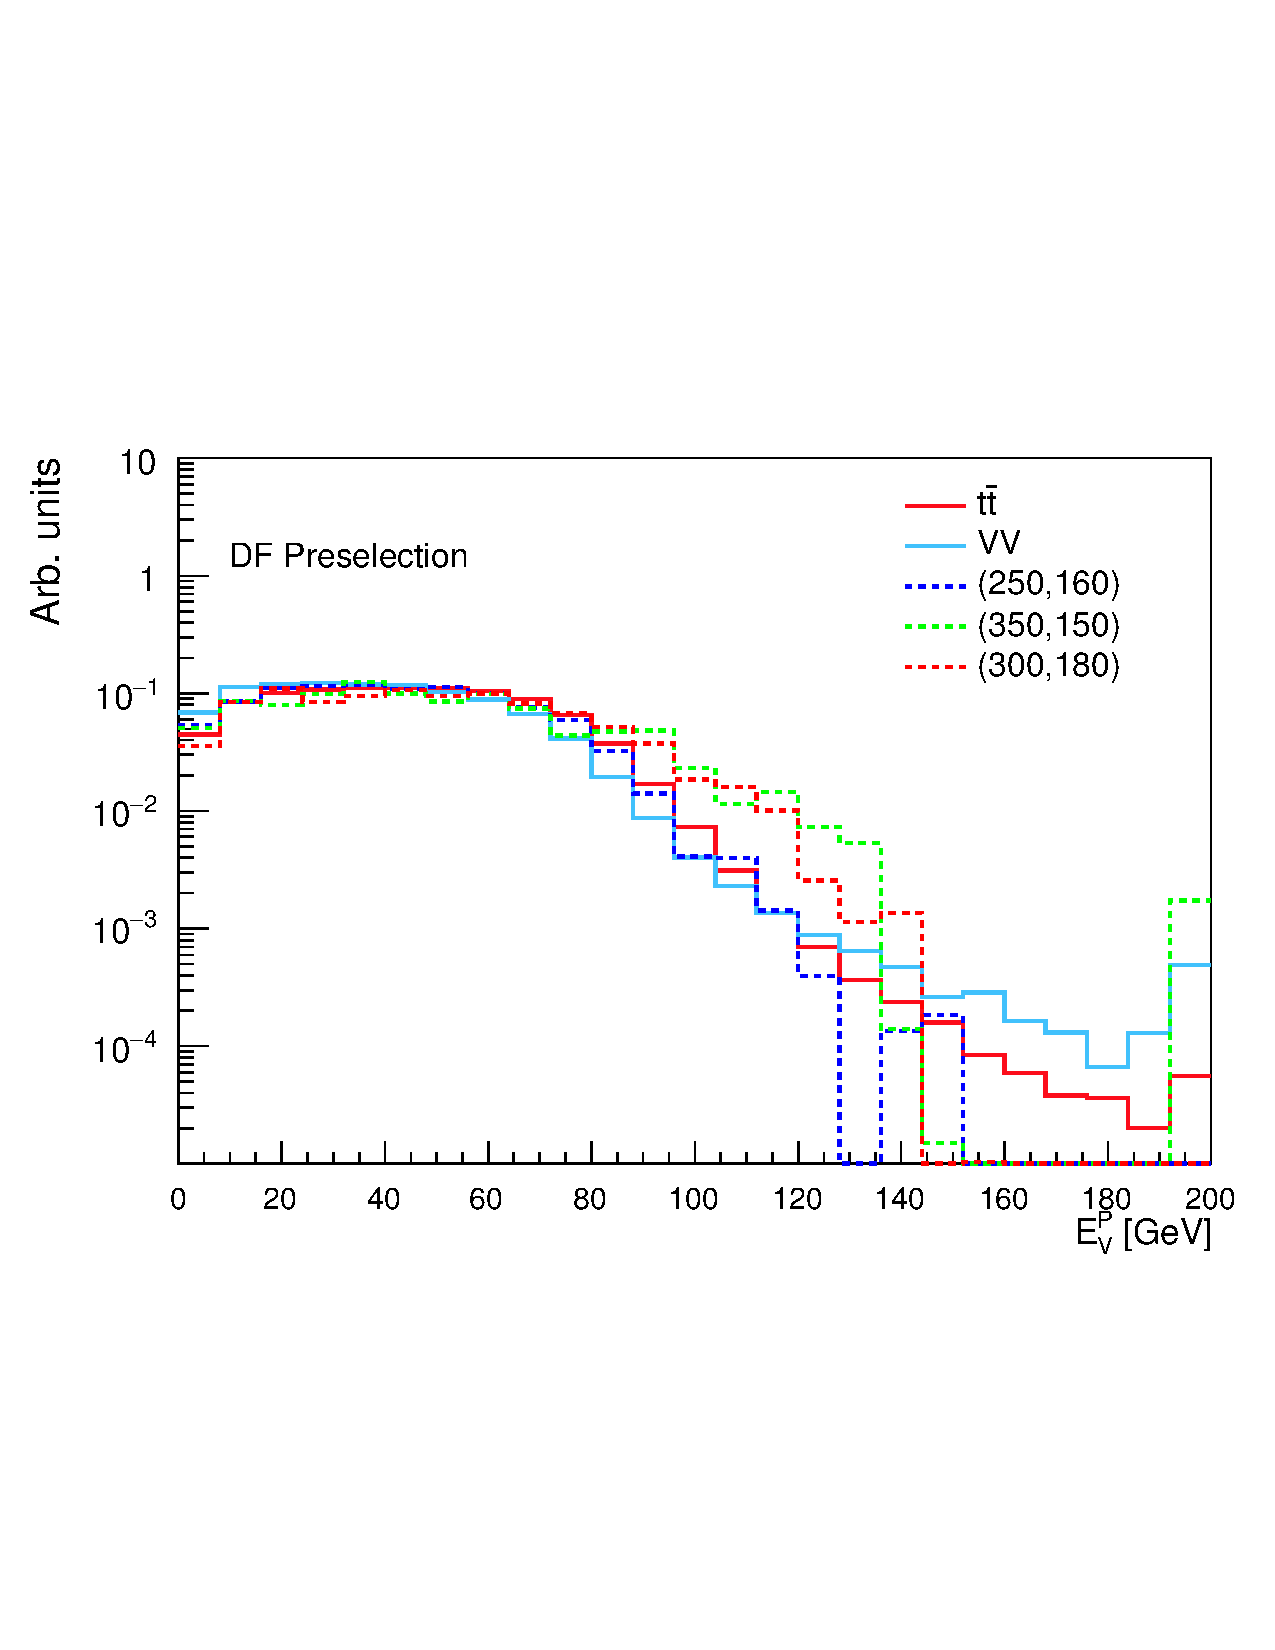
\includegraphics[width=0.7\textwidth]{figures/search_stop2l/strategy/comp_plots/dfpresel_MDR}
        \caption{
            Normalised distribution of the $\mdr$ variable for several $\stopone \rightarrow b W \ninoone$
            signal hypotheses, labeled with respect to their assumed $(m_{\stopone}, m_{\ninoone})$ values in the
            legend.
            The SM \ttbar~and diboson ($VV$) background processes are also shown for comparison.
        }
        \label{fig:rjr_MDR}
    \end{center}
\end{figure}

The next Jigsaw variable to be used is the so-called `visible shape' of the $PP$ (COM) frame.
In the limiting case of $m_{V_a} = m_{V_b} = 0$, in which the current analysis finds itself,
this quantity corresponds to the (inverse) boost factor ($\gamma$) associated with the boost from the
$PP$ frame to the $P_i$ frames and is defined as follows,
\begin{align}
    \text{PP Visible Shape} \rightarrow \gaminv \equiv \frac{
        \sqrt{
            2(|\vec{p}_{V_a}^{\,PP}| |\vec{p}_{V_b}^{\,PP}| + \vec{p}_{V_a}^{\,PP} \cdot \vec{p}_{V_b}^{\,PP})
        }
    }
    {
        |\vec{p}_{V_a}^{\,PP}| + |\vec{p}_{V_b}^{\,PP}|.
    }.
    \label{eq:rjr_gaminv}
\end{align}
The quantity \gaminv is a measure of how the two visible systems, $V_i$, are distributed.
It tends towards unity when $V_a$ and $V_b$ (the two leptons) are equal in momenta and collinear while tending
towards zero when they are back-to-back or having different momenta.
In this sense, the variable earns its name as a measure of the `visible shape' of the decay.
In decays with massive particles contributing to the missing transverse momentum,
the visible final state legs $V_a$ and $V_b$ will, on average, tend to not be back-to-back since,
in addition to balancing each other, they much balance the invisible particles.
This effect is exaggerated in two cases: (1) when the decay is highly `active' (as in \ttbar),
and (2) when the invisible system is composed of heavy particles.
The effect (1) is essentially due to our including in the states $V_a$ and $V_b$ only the
final state leptons: the quantity \gaminv is blind to any jets in the event and the `shape' it
corresponds to is in response to balancing these jets as well.
The effect (2) results in the visible legs recoiling harder off of the heavier invisible particles,
thus tending to be collinear.
Distributions of the \gaminv quantity are shown in Figure~\ref{fig:rjr_gaminv}.

\begin{figure}[!htb]
    \begin{center}
        \includegraphics[width=0.7\textwidth]{figures/search_stop2l/strategy/comp_plots/dfpresel_gamInvRP1}
        \caption{
            Normalised distribution of the $\gaminv$ variable for several $\stopone \rightarrow b W \ninoone$
            signal hypotheses, labeled with respect to their assumed $(m_{\stopone}, m_{\ninoone})$ values in the
            legend.
            The SM \ttbar~and diboson ($VV$) background processes are also shown for comparison.
        }
        \label{fig:rjr_gaminv}
    \end{center}
\end{figure}

The variables discussed so far are relatively independent of the underlying signal model
that we are attempting to search for.
Their utility relies simply on their being massive particles contributing to the missing
transverse momentum.

We now discuss a variable that, in order for it to be useful in the search for \stopone particles,
makes an assumption on the nature of the pair-produced sparticle that we are
searching for.
This variable, \cosb, is angular in nature that is sensitive to the decay angle of a given lepton with
respect to the beam axis in it's production frame.

We define \cosb using only the two final state leptons.
Each of the leptons is boosted into the frame of the dilepton system, after which
we take the difference in pseudorapidities of the leptons in this frame,
$\Delta \eta_{\ell \ell} = \eta^+ - \eta^-$, where $\eta^+$ ($\eta^-$) refers to the
pseudorapidity of the positively (negatively) charged lepton.
The quantity \cosb is then defined as,
\begin{align}
    \cosb = \tanh ( \Delta \eta_{\ell\ell} / 2),
    \label{eq:rjr_cosb}
\end{align}
and is discussed further in Ref.~\cite{Melia:2011cu}.
As \cosb is sensitive to the projection angle of the lepton from its parent \stopone, it is
sensitive to the spin of the \stopone.
This can be seen in Figure~\ref{fig:rjr_cosb}, where we see that for the decay of the
spin-zero \stopone, the angular distribution is flatter and peaks at 0.
For the SM \ttbar~and $WW$ backgrounds, however, \cosb tends to peak at values $\pm 1$.

\begin{figure}[!htb]
    \begin{center}
        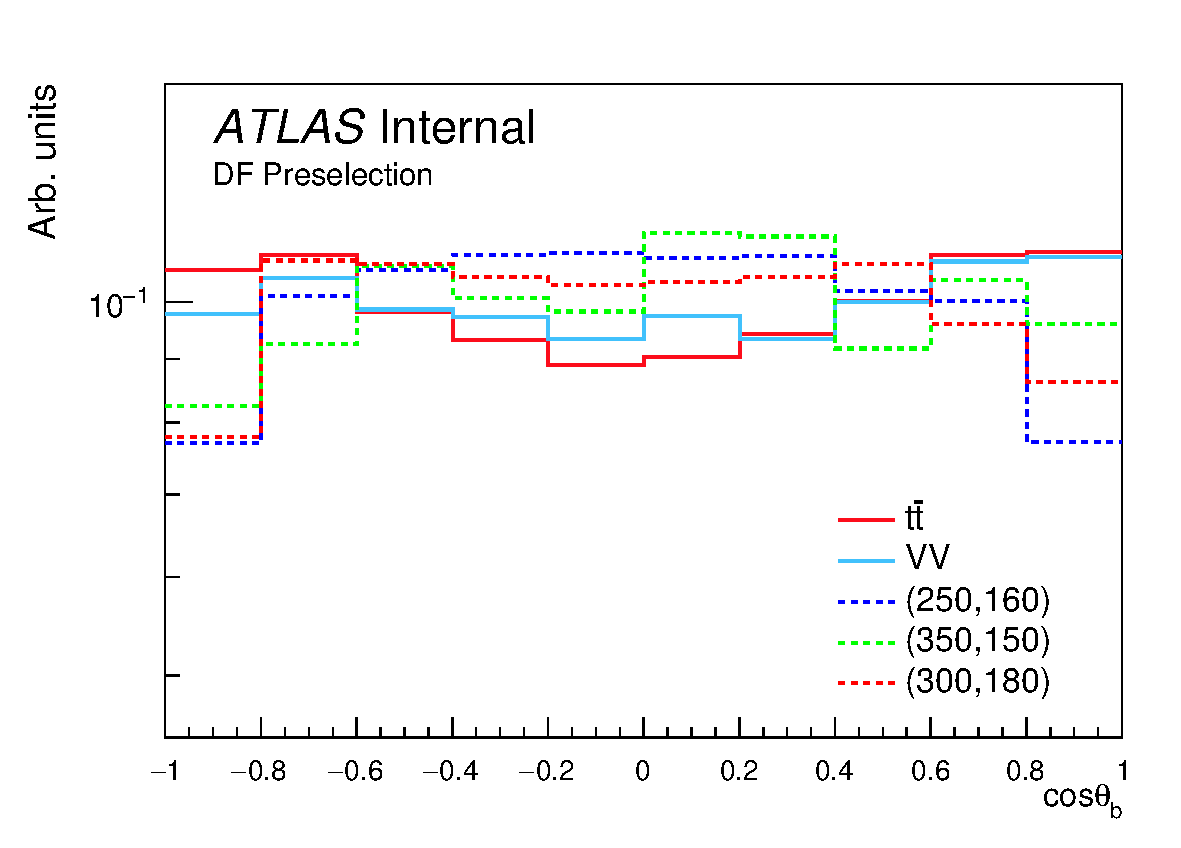
\includegraphics[width=0.7\textwidth]{figures/search_stop2l/strategy/comp_plots/dfpresel_cosThetaB}
        \caption{
            Normalised distribution of the $\cosb$ variable for several $\stopone \rightarrow b W \ninoone$
            signal hypotheses, labeled with respect to their assumed $(m_{\stopone}, m_{\ninoone})$ values in the
            legend.
            The SM \ttbar~and diboson ($VV$) background processes are also shown for comparison.
        }
        \label{fig:rjr_cosb}
    \end{center}
\end{figure}

In addition to the potential separation power between the decays of scalar \stopone particles
and the dominant SM backgrounds that \cosb exhibits in Figure~\ref{fig:rjr_cosb}, it should also
be noted that it is a longitudinally boost-invariant quantity.
It depends only on the \textit{difference} in pseudorapidities of the leptons, $\Delta \eta_{\ell\ell}$,
and thus is insensitive to our ignorance of the overall $z$-momenta in the event.
In this sense, the quantity \cosb follows very nicely the variables obtained from the RJR decay tree,
which are also motivated by longitudinal (and contra-) boost invariance.

\FloatBarrier
%%%%%%%%%%%%%%%%%%%%%%%%%%%%%%%%%%%%%%%%%%%%%%%%%%%%%%%%%%%%%%%%%%%%%%%%%%%
%%%%%%%%%%%%%%%%%%%%%%%%%%%%%%%%%%%%%%%%%%%%%%%%%%%%%%%%%%%%%%%%%%%%%%%%%%%
%%%%%%%%%%%%%%%%%%%%%%%%%%%%%%%%%%%%%%%%%%%%%%%%%%%%%%%%%%%%%%%%%%%%%%%%%%%
%
% SR DEF
%
%%%%%%%%%%%%%%%%%%%%%%%%%%%%%%%%%%%%%%%%%%%%%%%%%%%%%%%%%%%%%%%%%%%%%%%%%%%
%%%%%%%%%%%%%%%%%%%%%%%%%%%%%%%%%%%%%%%%%%%%%%%%%%%%%%%%%%%%%%%%%%%%%%%%%%%
%%%%%%%%%%%%%%%%%%%%%%%%%%%%%%%%%%%%%%%%%%%%%%%%%%%%%%%%%%%%%%%%%%%%%%%%%%%
\subsection{Signal Region Definitions}
\label{sec:stop_signal_region}

The definition of the SRs in the search for the three-body decay of the \stopone revolve around
two observations:
\begin{enumerate}
    \item The $\stopone \rightarrow b W \ninoone$ kinematics change rapidly as one traverses from
        the region near $\sdiff~ = m_{\text{top}}$ to that of $\sdiff~ = ~m_W$,
        as illustrated in Figure~\ref{fig:stop_phase_space}
    \item The angular quantities \cosb and \dpb,  sensitive to the presence of the scalar \stopone and massive
        \ninoone, respectively, allow for tight separation between the \stopone signal and dominant
        SM background processes
\end{enumerate}
The first item will ultimately result in the definition of two orthogonal SRs, one generally
more sensitive to the $\bWN$ decays nearer to the $\sdiff = m_{\text{top}}$ boundary
and the other being sensitive to those nearer to the $\sdiff = m_W$ boundary.
The primary method for defining SRs targeting these differing regimes is motivated by Figure~\ref{fig:stop_nbjets},
which shows that the \bWN decays with $\sdiff$ nearer to $m_W$, the reconstructed $b$-tagged
jet multiplicity tends to 0.
For this reason, the SRs targeting the $\sdiff \rightarrow m_W$ will require that the
candidate events have zero $b$-tagged jets, i.e. they apply a $b$-tagged jet \textit{veto} (`$b$-veto').
The SRs targeting the $\sdiff \rightarrow m_{\text{top}}$, on the other hand, will
require that there be at least one $b$-tagged jet in the candidate events.

The second item listed above is best illustrated by the distribution in Figure~\ref{fig:stop_corr2d_bveto}.
These two-dimensional distributions illustrate that the \bWN signal tends to populate
a different region in the two-dimensional space defined by $(\cosb, \dpb)$ than
the dominant dilepton SM backgrounds composed of \ttbar~and diboson production.
For this reason, the SRs will be further characterised by applying a selection within
the two-dimensional basis defined by the \cosb and \dpb variables.
Figure~\ref{fig:stop_corr2d_b} shows similar distributions as those presented in Figure~\ref{fig:stop_corr2d_bveto},
but illustrates that the relationship observed in the latter persist after
requiring that there be $b$-tagged jets in the events (the former distributions require a $b$-veto).
The fact that the $(\cosb, \dpb)$ relationship holds roughly independent of the $b$-tagged
jet multiplicity means that the same selection in this two-dimensional plane
can be applied for the SRs targeting both \bWN regimes, $\sdiff \rightarrow m_W$ and
$\sdiff \rightarrow m_{\text{top}}$.


\begin{figure}[!htb]
    \begin{center}
        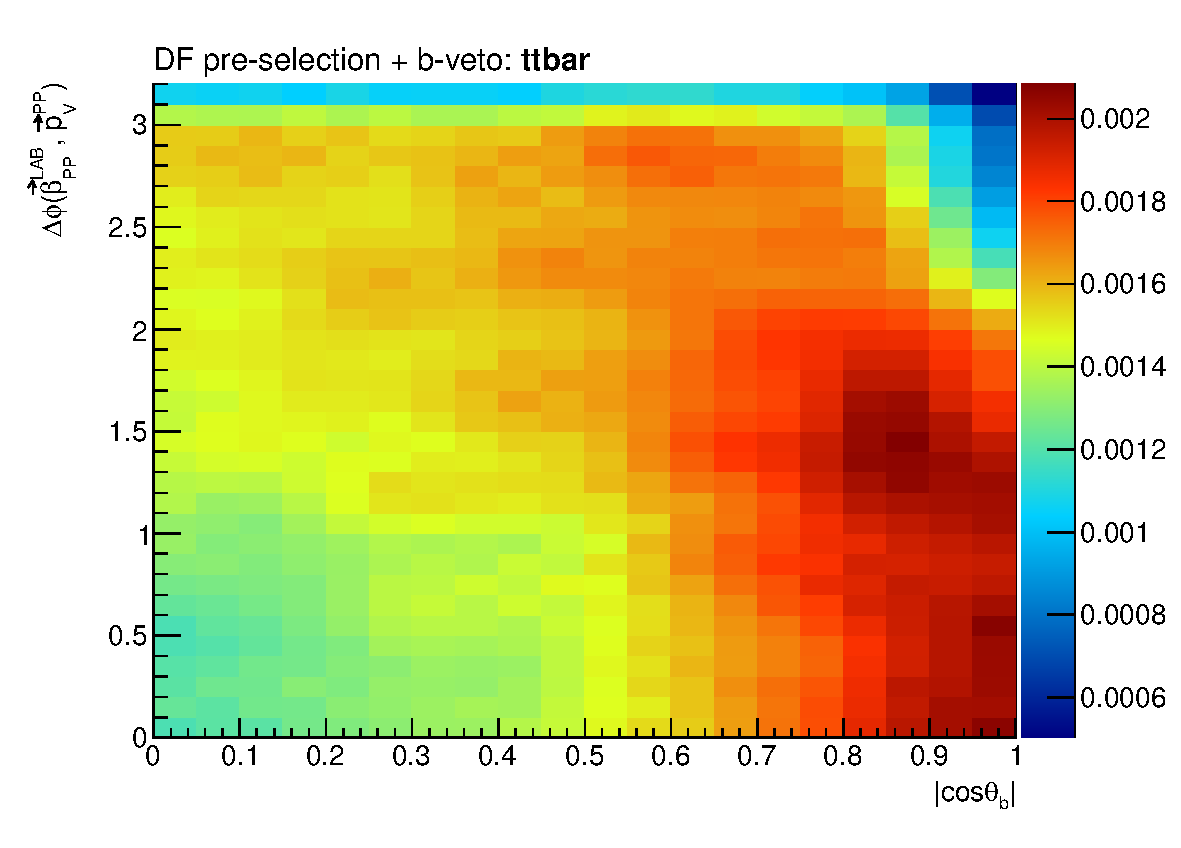
\includegraphics[width=0.48\textwidth]{figures/search_stop2l/strategy/corr2d/wwbveto_cosThetaB_DPB_vSS_ttbar_2d}
        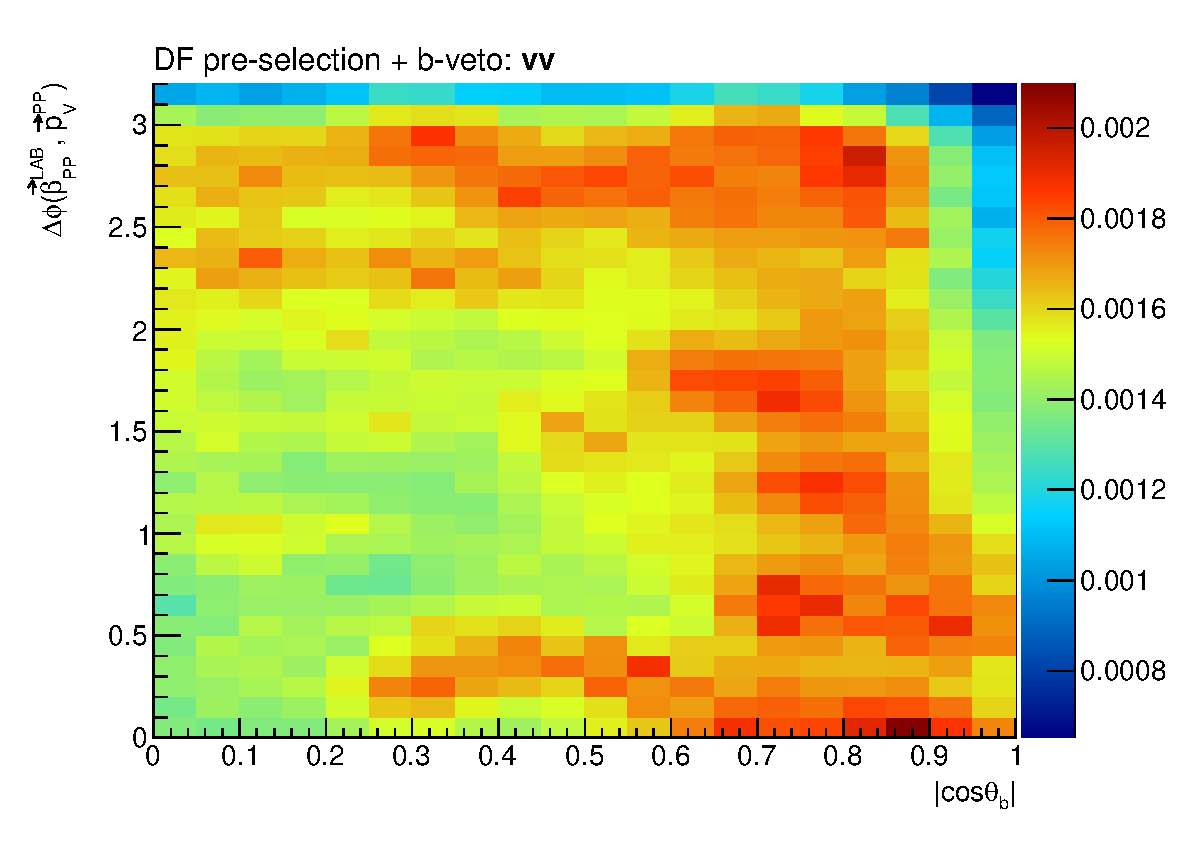
\includegraphics[width=0.48\textwidth]{figures/search_stop2l/strategy/corr2d/wwbveto_cosThetaB_DPB_vSS_vv_2d}
        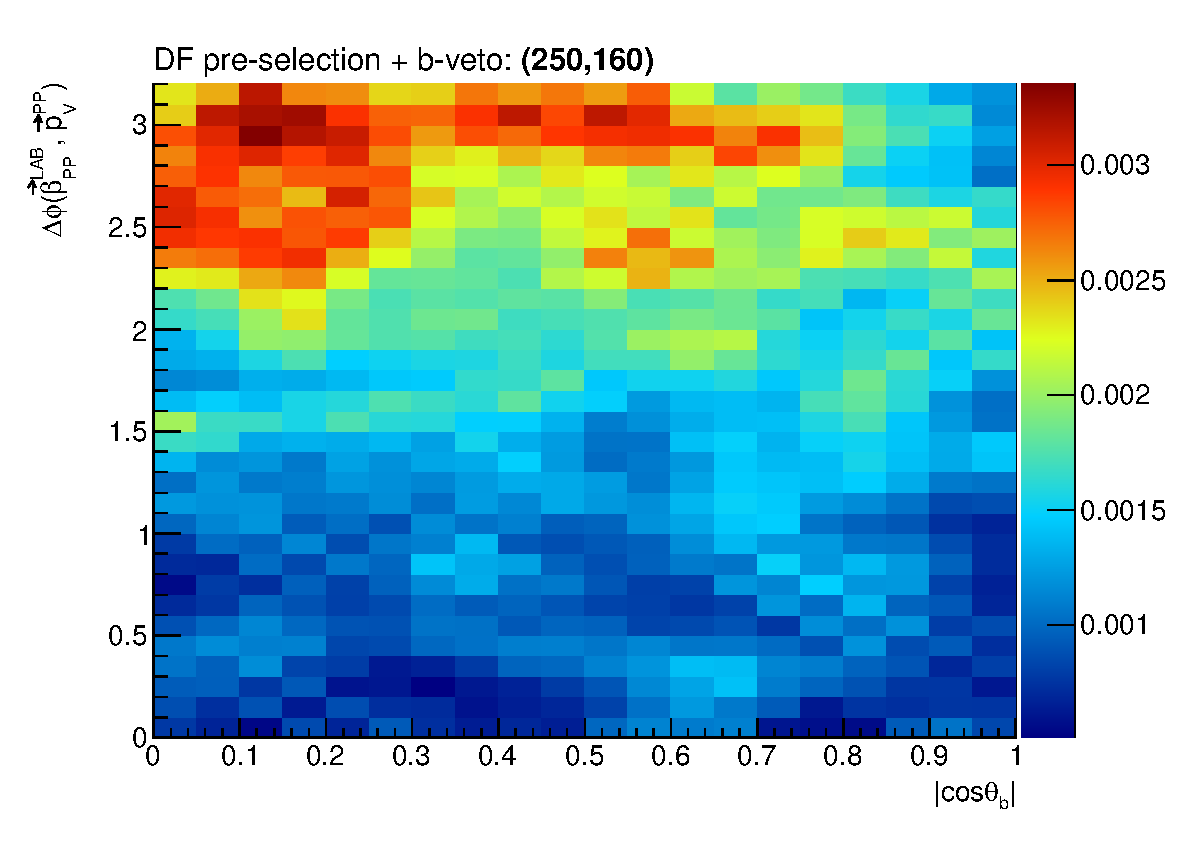
\includegraphics[width=0.48\textwidth]{figures/search_stop2l/strategy/corr2d/wwbveto_cosThetaB_DPB_vSS_bwn250_160_2d}
        \caption{
            Two-dimensional relationship between \dpb and \cosb for SM \ttbar~(\textit{\textbf{upper left}}),
            SM diboson processes (\textit{\textbf{upper right}}), and the \bWN decay with $\msn = (250, 160)$\,GeV
            (\textit{\textbf{bottom}}).
            The selection applied to the events populating these distributions follows the DF Preselection outlined in Table~\ref{tab:stop_preselection}
            with the additional requirement that there be no $b$-tagged jets in the event.
            The distributions are normalized, so only the shapes are relevant for comparison.
        }
        \label{fig:stop_corr2d_bveto}
    \end{center}
\end{figure}

\begin{figure}[!htb]
    \begin{center}
        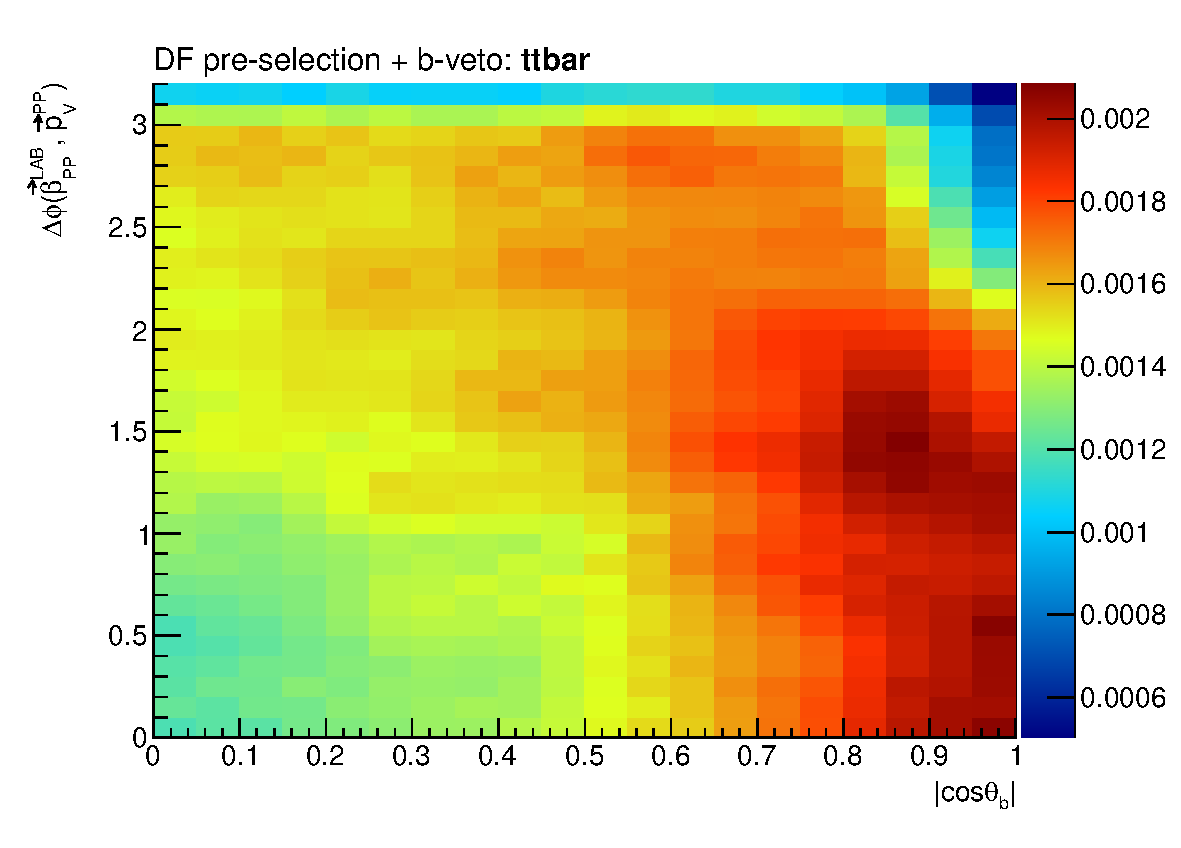
\includegraphics[width=0.48\textwidth]{figures/search_stop2l/strategy/corr2d/wwbveto_cosThetaB_DPB_vSS_ttbar_2d}
        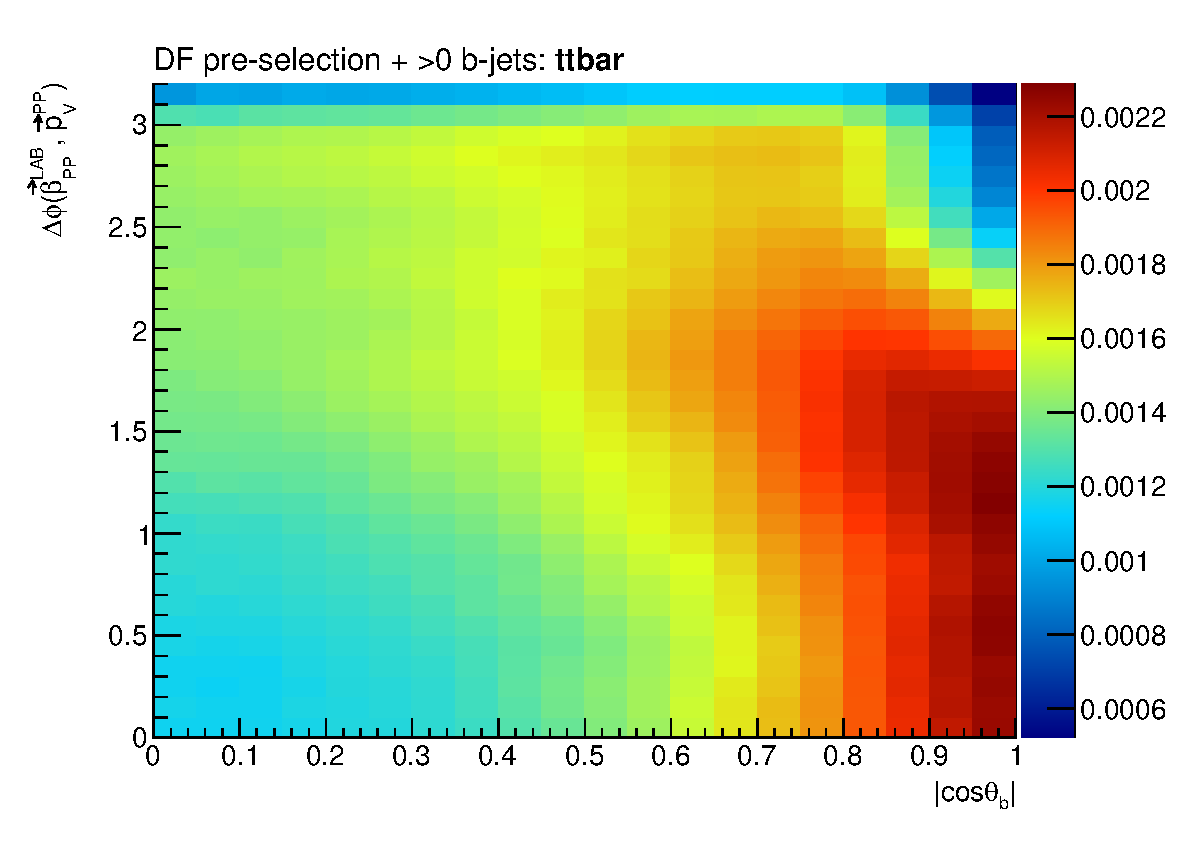
\includegraphics[width=0.48\textwidth]{figures/search_stop2l/strategy/corr2d/wwb_cosThetaB_DPB_vSS_ttbar_2d}
        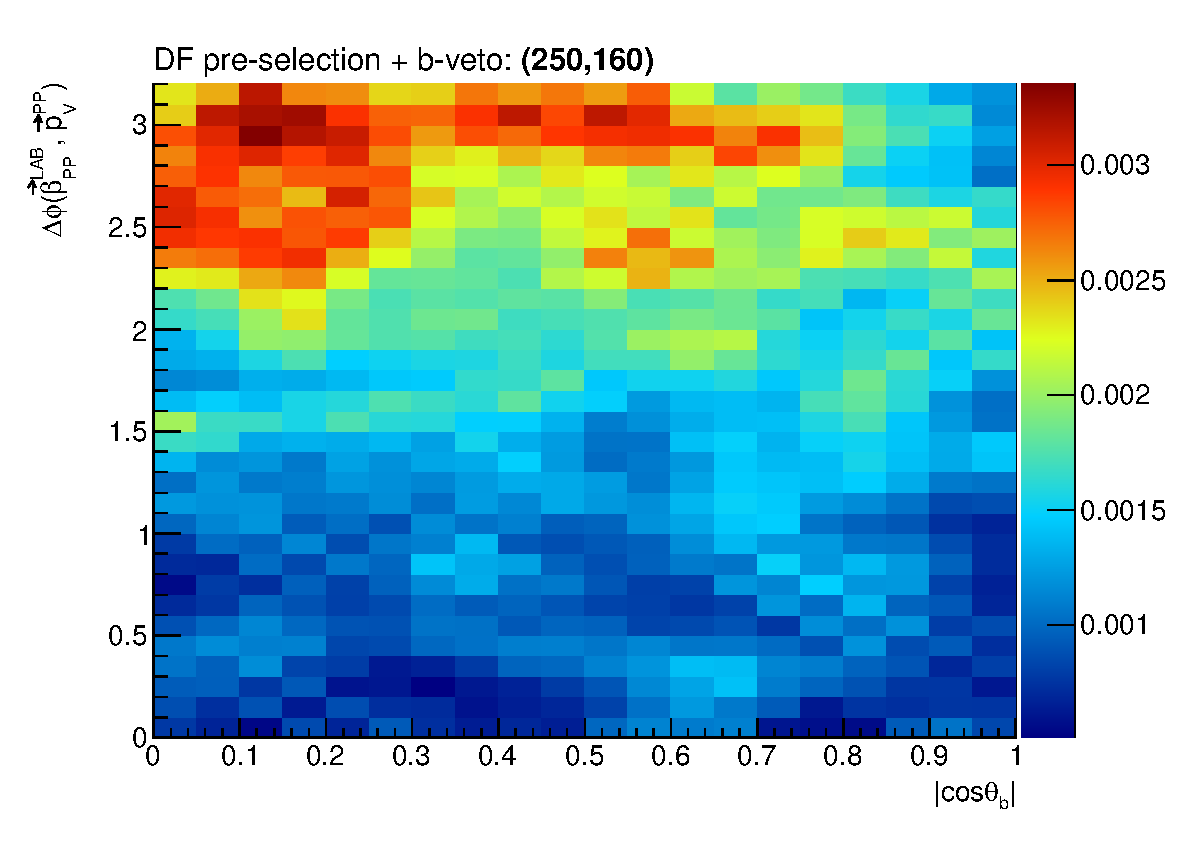
\includegraphics[width=0.48\textwidth]{figures/search_stop2l/strategy/corr2d/wwbveto_cosThetaB_DPB_vSS_bwn250_160_2d}
        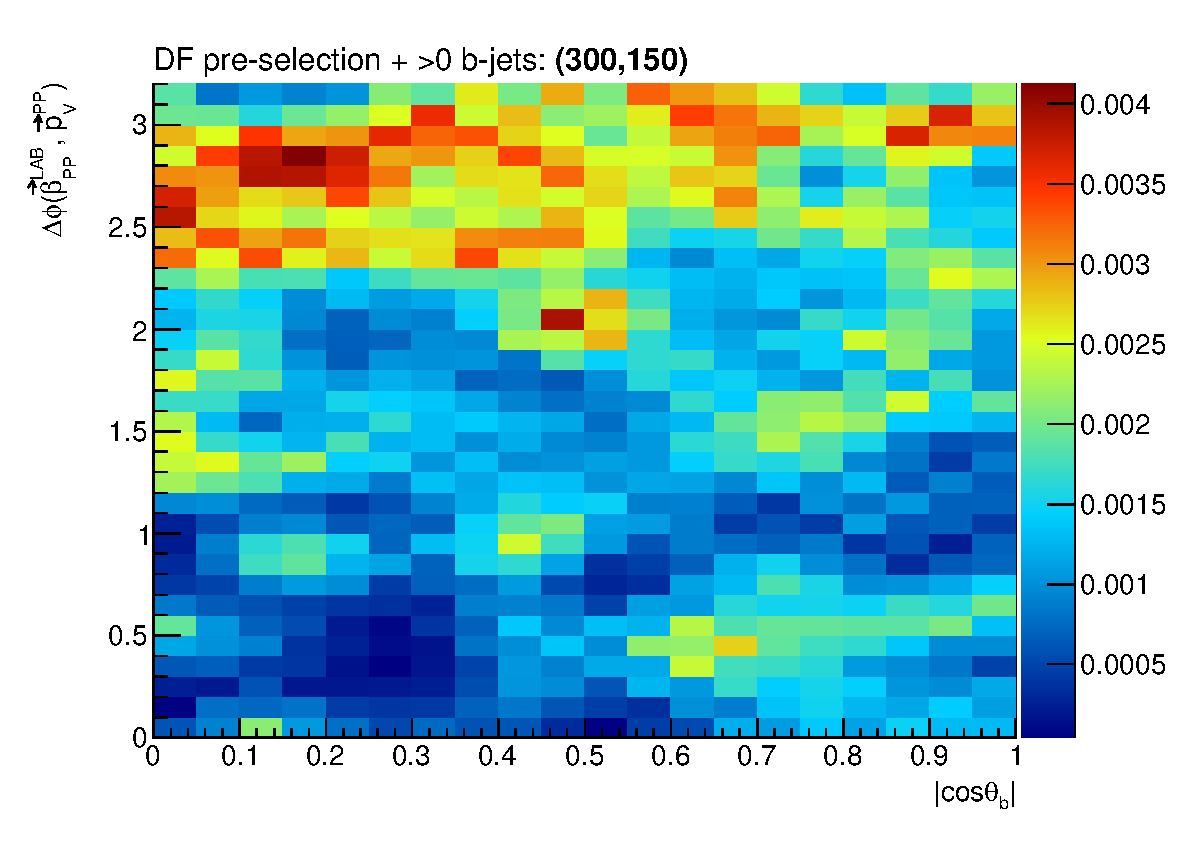
\includegraphics[width=0.48\textwidth]{figures/search_stop2l/strategy/corr2d/wwb_cosThetaB_DPB_vSS_bwn300_150_2d}
        \caption{
            Two-dimensional relationship between \dpb and \cosb for SM \ttbar~(\textit{\textbf{upper}}),
            the \bWN decay with $\msn = (250, 160)$\,GeV (\textit{\textbf{lower left}}),
            and the \bWN decay with $\msn = (350, 150)$\,GeV (\textit{\textbf{lower right}}).
            The selection applied to the events populating these distributions are
            required to satisfy the DF Preselection outlined in Table~\ref{tab:stop_preselection},
            with those on the left having an additional requirement that there be no $b$-tagged
            jets in the events and those on the right requiring that there be at least one $b$-tagged
            jet in the event.
            The distributions are normalized, so only the shapes are relevant for comparison.
        }
        \label{fig:stop_corr2d_b}
    \end{center}
\end{figure}

With the above discussion in mind, the complete basis of observables used to define the SRs are given by
the following,
\begin{table}[!htb]
    \begin{center}
        \caption{
            Basis of kinematic observables for the definition of analysis regions
            in the \bWN search.
        }
        \label{tab:stop_basis}
        \begin{tabular}{c}
            \hline
            \hline
                \rpt \\
                \gaminv \\
                \cosb \\
                \dpb \\
                \mdr \\
                $b$-tagged jet multiplicity \\
            \hline
            \hline
        \end{tabular}
    \end{center}
\end{table}

\FloatBarrier
\subsubsection{Optimization Procedure}
\label{sec:stop_opt}

In order to choose the precise selection thresholds on the quantities listed in Table~\ref{tab:stop_basis},
an optimization procedure is followed.
The procedure used in the search for the \bWN decay is a brute force method, and is as follows.
A multi-dimensional scan is performed over the subset of those quantities in listed in Table~\ref{tab:stop_basis},
which are listed in Table~\ref{tab:stop_opt_scan_vars}.
The scan is done using objects (leptons and jets) that satisfy the signal level criteria,
detailed in Tables~\ref{tab:stop_lepton_def} and \ref{tab:stop_jet_def}.

\begin{table}[!htb]
    \begin{center}
        \caption{
            Kinematic observables used in the \bWN grid search optimization procedure.
        }
        \label{tab:stop_opt_scan_vars}
        \begin{tabular}{c}
            \hline
            \hline
                \rpt \\
                \gaminv \\
                m \\
                b \\
            \hline
            \hline
        \end{tabular}
    \end{center}
\end{table}
\noindent
In Table~\ref{tab:stop_opt_scan_vars}, the quantities `m' and `b' are related to the slope and y-intercept of the line in the two-dimensional
space $(\cosb, \dpb)$, as illustrated in Figure~\ref{fig:stop_2d_opt}.
\begin{figure}[!htb]
    \begin{center}
        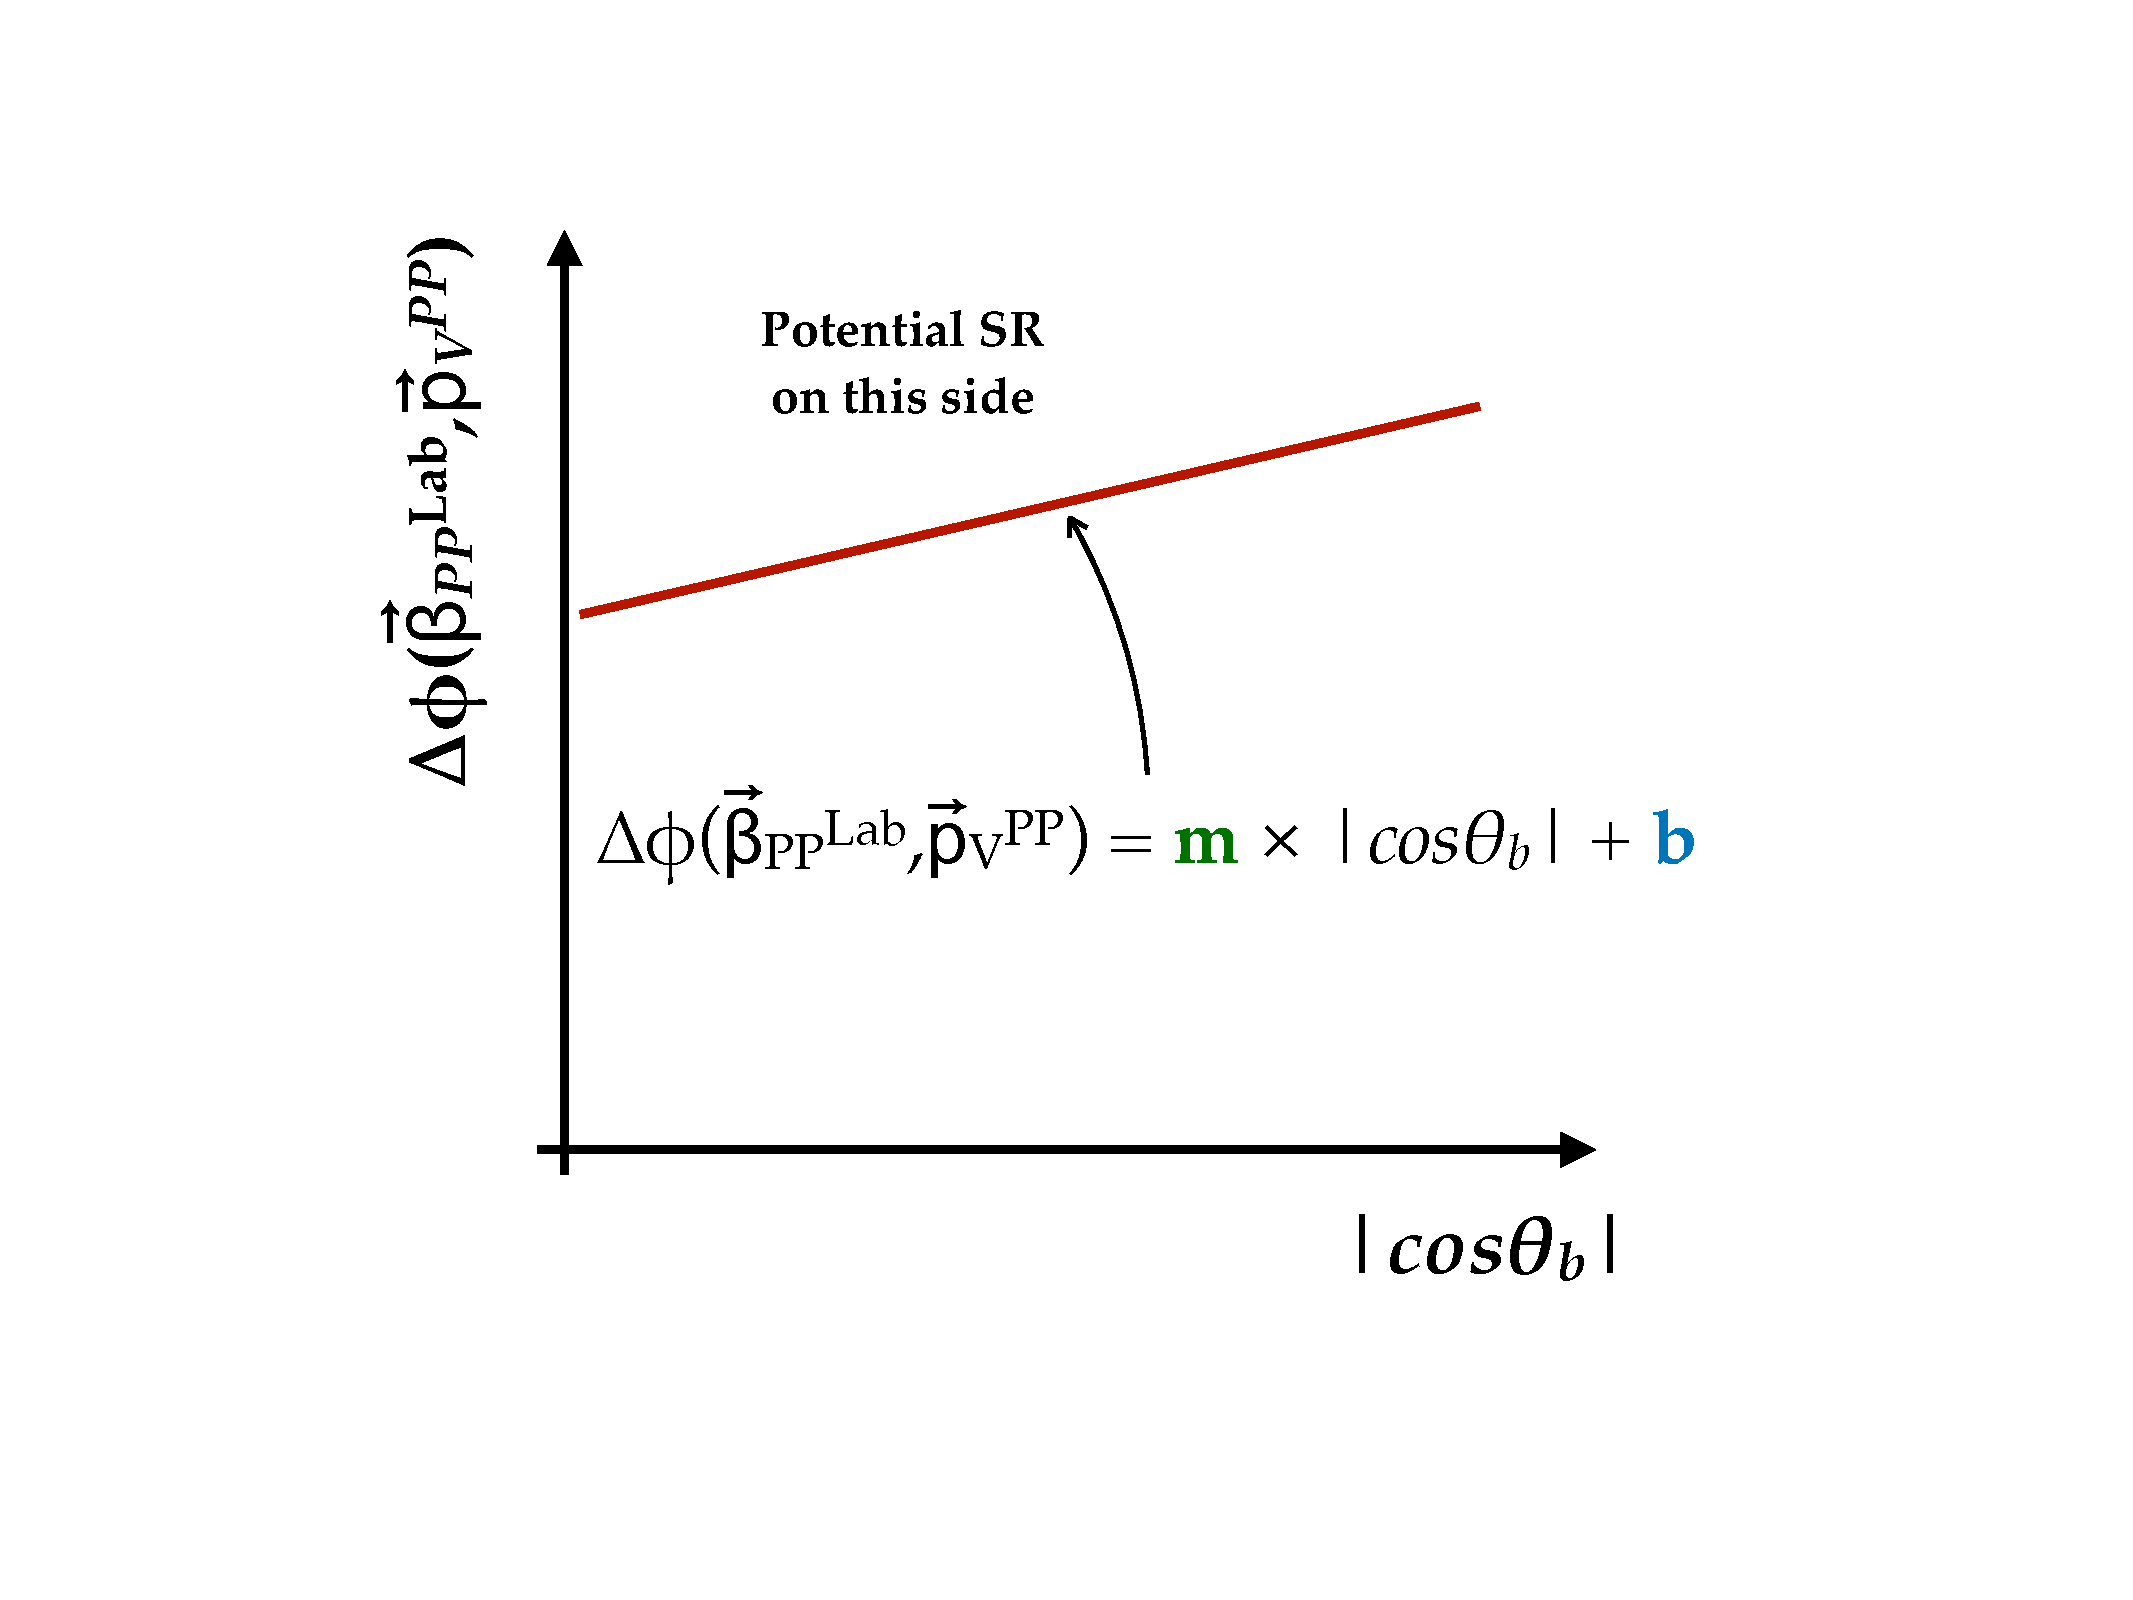
\includegraphics[width=0.5\textwidth]{figures/search_stop2l/strategy/stop_2d_optPDF}
        \caption{
            Illustration of the two-dimensional selection in the $(\cosb, \dpb)$-plane.
        }
        \label{fig:stop_2d_opt}
    \end{center}
\end{figure}
For each of the quantities in Table~\ref{tab:stop_opt_scan_vars}, a fine-grained set of threshold
steps is defined and a multi-dimensional scan over all allowed step values for all four quantities
is performed.
At each step, a region is defined with the requirements as follows,
\begin{align*}
            \rpt &> \text{step}_{\{\rpt\}} \\
            \gaminv &> \text{step}_{\{\gaminv\}} \\
            \text{m} &= \text{step}_{\{\text{m}\}} \\
            \text{b} &= \text{step}_{\{\text{b}\}},
\end{align*}
and a metric for evaluating the sensitivity to the \bWN process of the given region
is calculated.
The metric used in the search for the \bWN process is an approximation to the Gaussian significance
associated with the discovery $p_0$-value.
The larger this quantity is, the larger the expected sensitivity to the given \bWN decay.
The significance is computed using the \textsc{RooStats} library and takes as input
the predicted number of signal events, the predicted number of background events,
and a level of uncertainty on the background event yield.\footnote{The precise
significance metric used is \href{https://root.cern.ch/doc/v606/namespaceRooStats_1_1NumberCountingUtils.html\#a4ac05df7796855dca2d8b24473bf7d4e}{RooStats::NumberCountingUtils::BinomialObsZ} 
}
Since the actual background uncertainty is unknown at the point of designing an analysis'
search regions, it is usually taken to be a conservative value.
In the search described here, the relative background uncertainty, $\Delta b_{\text{opt}}$, was taken to be,
\begin{align*}
    \Delta b_{\text{opt}} = \sqrt{ (0.30)^2 + (\delta s)^2 },
\end{align*}
where $\delta s$ is the relative statistical uncertainty on the MC-simulated signal sample.
The quantity $\delta s$ is added in order to act as a penalty term for cases in which the
MC statistics in the signal sample become too small to give reliable estimates of the significance.

The optimisation scan is performed using only the dominant expected backgrounds, SM \ttbar~ and diboson production,
as input.
For the signal samples used to provide the estimated signal yield input,
the scan is performed three times for each of the three \textit{benchmark} signal samples with $\msn = (250, 160)$, $(300,150)$, and $(300,120)$\,GeV,
in order to assess how well each of the regions in the step procedure perform
across the three-body phase space with differing values for $\sdiff$.

At the end of the scan, there are $\mathcal{O}(10^4)$ different regions checked.
The best region is chosen based on its maximization of the significance metric as well as
maintaining that there be at most 30\% statistical uncertainty on the signal and background MC samples
once the selection for the associated region is applied.
This choice is made taking into account the three benchmark \bWN signal scenarios, with the hope
of obtaining a continuous sensitivity throughout the three-body regime for scenarios
with different values of $\sdiff$.

\begin{table}[!htb]
    \begin{center}
        \caption{
            Final values obtained after performing the brute-force scan
            over the parameters listed in Table~\ref{tab:stop_opt_scan_vars}.
        }
        \label{tab:stop_scan_results}
        \begin{tabular}{l | c}
            \hline
            \hline
                \textbf{Quantity} & \textbf{Final Value Obtained from Scan} \\
                \hline
                \rpt & $0.7$ \\
                \gaminv & $0.7$ \\
                m   & $0.9$ \\
                b   & $1.6$ \\
            \hline
            \hline
        \end{tabular}
    \end{center}
\end{table}

%%%%%%%%%%%%%%%%%%%%%%%%%%%%%%%%%%%%%%%%%%%%%%%%%%%%%%%%%%%%%%%%%%%%%%%%%%%
%%%%%%%%%%%%%%%%%%%%%%%%%%%%%%%%%%%%%%%%%%%%%%%%%%%%%%%%%%%%%%%%%%%%%%%%%%%
%%%%%%%%%%%%%%%%%%%%%%%%%%%%%%%%%%%%%%%%%%%%%%%%%%%%%%%%%%%%%%%%%%%%%%%%%%%
%
% SR DEF
%
%%%%%%%%%%%%%%%%%%%%%%%%%%%%%%%%%%%%%%%%%%%%%%%%%%%%%%%%%%%%%%%%%%%%%%%%%%%
%%%%%%%%%%%%%%%%%%%%%%%%%%%%%%%%%%%%%%%%%%%%%%%%%%%%%%%%%%%%%%%%%%%%%%%%%%%
%%%%%%%%%%%%%%%%%%%%%%%%%%%%%%%%%%%%%%%%%%%%%%%%%%%%%%%%%%%%%%%%%%%%%%%%%%%
\subsubsection{Final Signal Region Definitions}

On top of the selections defined as a result of the brute-force scan, listed in Table~\ref{tab:stop_scan_results},
an \mdr requirement is added.
As the kinematic endpoint of the \mdr variable is sensitive to the (squared) mass differences
between the \stopone and \ninoone (c.f. Equation~\ref{eq:mdr_endpoint}), it is expected that the specific cut value on this
quantity will be lower for the \bWN decay scenarios with lower values of \sdiff.
The specific values of \mdr are determined by running a similar optimisation scan as detailed
in the previous section, but with only the \mdr quantity being scanned over
and with all other cuts fixed to those detailed in Table~\ref{tab:stop_scan_results}.
This is done twice, once for the benchmark signal point with $\msn = (250,160)$\,GeV and
a second time with $\msn = (350,120)$\,GeV.
The former (latter) defines the \mdr cut used for the SR targeting the \bWN decay scenarios with
$\sdiff$ nearer to $m_W$ ($m_{\text{top}}$).

The final SR definitions used in for the search for the three-body decay of the \stopone
are detailed in Table~\ref{tab:stop_sr_def}.
There are four SRs defined in total, two of which target the $\sdiff~\rightarrow~m_W$ region
and two target the $\sdiff~=~m_{\text{top}}$ region.
The former are defined by a $b$-tagged jet veto, and the latter are inclusive of
events with $b$-tagged jets.
Within each of these two categories, the SRs are further broken down by the dilepton flavor:
whether the two leptons in the events have the same-flavor (SF) or different-flavor (DF).
In order to reduce backgrounds in which the two leptons arise from the decays of $Z$-bosons,
a $Z$-veto is applied to the SF SRs by requiring that the dilepton invariant mass be outside
a 20\,\GeV window centered on the $Z$-boson mass.

The total expected background yield and composition in terms of specific SM processes
is given in Table~\ref{tab:stop_exp_sr_yield} for each of the SRs defined in Table~\ref{tab:stop_sr_def}.
It can be seen, as assumed in the text so far, that SM \ttbar~and diboson production processes
are expected to be the main SM processes contaminating the SRs.

\begin{table}[!htb]
    \begin{center}
        \caption{
            Final signal region definitions for the \bWN search.
            Selections are made after the pre-selection requirements defined in Table~\ref{tab:stop_preselection}.
            The quantities `m' and `b' are illustrated in Figure~\ref{fig:stop_2d_opt} and refer to the two-dimensional selection:
                $\dpb > \text{m} \times |\cosb| + \text{b}$.
            The lepton \pT~requirements are chosen so as to be on the dilepton trigger efficiency
            plateau.
        }
        \label{tab:stop_sr_def}
        \begin{scriptsize}
        \begin{tabular}{l | c  c  c  c}
            \hline
            \hline
            \multicolumn{5}{c}{\textbf{Signal Region Definitions for the \bWN Search}} \\
            \hline
                    & \multicolumn{4}{c}{\textbf{Common Selection}} \\
            \hline
            Lead lepton \pT [GeV] & \multicolumn{4}{c}{$>25$} \\
            Sub-lead lepton \pT [GeV] & \multicolumn{4}{c}{$>20$} \\
            \rpt    & \multicolumn{4}{c}{$>0.7$} \\
            \gaminv & \multicolumn{4}{c}{$>0.7$} \\
            m   & \multicolumn{4}{c}{$0.9$} \\
            b   & \multicolumn{4}{c}{$1.6$} \\
            \hline
                & \multicolumn{1}{c|}{\textbf{SRw-SF}} & \multicolumn{1}{c|}{\textbf{SRw-DF}} & \multicolumn{1}{c|}{\textbf{SRt-SF}} & \textbf{SRt-DF} \\
            \hline
            Dilepton invariant mass, $m_{\ell\ell}$ [GeV] & $|m_{\ell\ell} - 91.2| > 20$ & \multicolumn{1}{c|}{no req.} & $|m_{\ell\ell} - 91.2| > 20$ & no req. \\
            $b$-tagged jet multiplicity & \multicolumn{2}{c|}{Exactly 0} & \multicolumn{2}{c}{$>0$} \\
            \mdr    & \multicolumn{2}{c|}{$>95$} & \multicolumn{2}{c}{$>110$} \\
            \hline
            \hline
        \end{tabular}
        \end{scriptsize}
    \end{center}
\end{table}

\begin{table}[!htb]
    \begin{center}
        \caption{
            Expected SM background processes in the SRs for the \bWN search,
            defined in Table~\ref{tab:stop_sr_def}.
            The bottom two rows show the predicted yields for two of the
            \bWN benchmark scenarios.
            The errors on the quoted yields are due to statistical and
            systematic uncertainties.
        }
        \label{tab:stop_exp_sr_yield}
        \begin{scriptsize}
        \begin{tabular}{l | c c c c}
            \hline
            \hline
                \textbf{Process}    & \textbf{SRw-SF} & \textbf{SRw-DF} & \textbf{SRt-SF} & \textbf{SRt-DF} \\
            \hline
            Total Expected SM & $10.94 \pm 3.60$ & $8.74 \pm 3.45$ & $3.00 \pm 1.59$ & $4.62 \pm 2.38$ \\
            \hline
            \ttbar  & $4.32 \pm 2.42$ & $4.73 \pm 2.82$         & $2.41 \pm 1.54$ & $3.38 \pm 2.31$ \\
            Single-top & $0.31 \pm 0.19$ & $0.23 \pm 0.07$      & $0.12 \pm 0.015$ & $0.15 \pm 0.09$  \\
            Diboson & $3.76 \pm 1.71$ & $3.03 \pm 1.33$         & $0.16 \pm 0.05$ & $0.00 \pm 0.00$ \\
            $Z$+jets & $1.52 \pm 0.79$ & $0.05 \pm 0.01$        & $0.10 \pm 0.03$ & $0.00 \pm 0.00$  \\
            $\ttbar+V$ & $0.04 \pm 0.01$ & $0.11\pm 0.03$       & $0.21 \pm 0.06$ & $0.24 \pm 0.09$ \\
            Fakes & $0.99 \pm 0.52$ & $0.59 \pm 0.29$           & $0.00 \pm 0.00$ & $0.82 \pm 0.23$ \\
            \hline
            \bWN, $\msn = (250,160)$\,GeV & $15.06 \pm 1.78$ & $18.93 \pm 1.86$ & $3.34 \pm 0.84$ & $4.06 \pm 0.97$ \\
            \bWN, $\msn = (300,150)$\,GeV & $4.47\pm1.09$ & $7.03 \pm 1.45$ & $11.43 \pm 2.00$ & $12.86 \pm 1.97$  \\
            \hline
            \hline
        \end{tabular}
        \end{scriptsize}
    \end{center}
\end{table}


\section{Estimation of Backgrounds}
\label{sec:stop_background_estimate}

In this section, we describe the methods used for the estimation of the SM background
contamination in the SRs.
By Table~\ref{tab:stop_exp_sr_yield}, it can be seen that the expected SM background
contamination to the SRs in the \bWN search is primarily composed of events
from the \ttbar~and diboson processes.
Given that these are the dominant backgrounds for the analysis, their estimation is performed
using the control region method, described in Section~\ref{sec:control_region_method}.
That is, dedicated CRs and VRs are defined for each of the two processes in order
to provide a normalisation correction for their MC prediction in the SRs.
All other background processes, being subdominant, have their predicted contribution
to the SR background taken directly from the MC simulation.
The estimation of the contribution of sources leading to fake and non-prompt leptons
is performed using the Matrix Method, described in Section~\ref{sec:matrix_method}.

Sections~\ref{sec:stop_ttbar_estimate} and \ref{sec:stop_vv_estimate} describe
the background estimate for the \ttbar~and diboson processes, respectively.

%sub-dominant and FNP via MC alone (shape and normalisation prediction)
%dominant, ttbar and vv, are estimated in a semi-data driven fashion using
% dedicated control regions
%  --> yields tables in CR
%  --> SR normalisation correction factors

The CR and VR definitions for both the \ttbar~and diboson background are based on the
SR definitions given in the previous section.
The CRs are defined primarily by inverting the two-dimensional selection
made in the $(\cosb, \dpb)$-plane, and maintaining similar selections as in the SRs for the other variables.
The VRs, on the other hand, are defined by inverting the selections on the non-angular variables relative to those
made in the SRs.

\begin{figure}[!htb]
    \begin{center}
        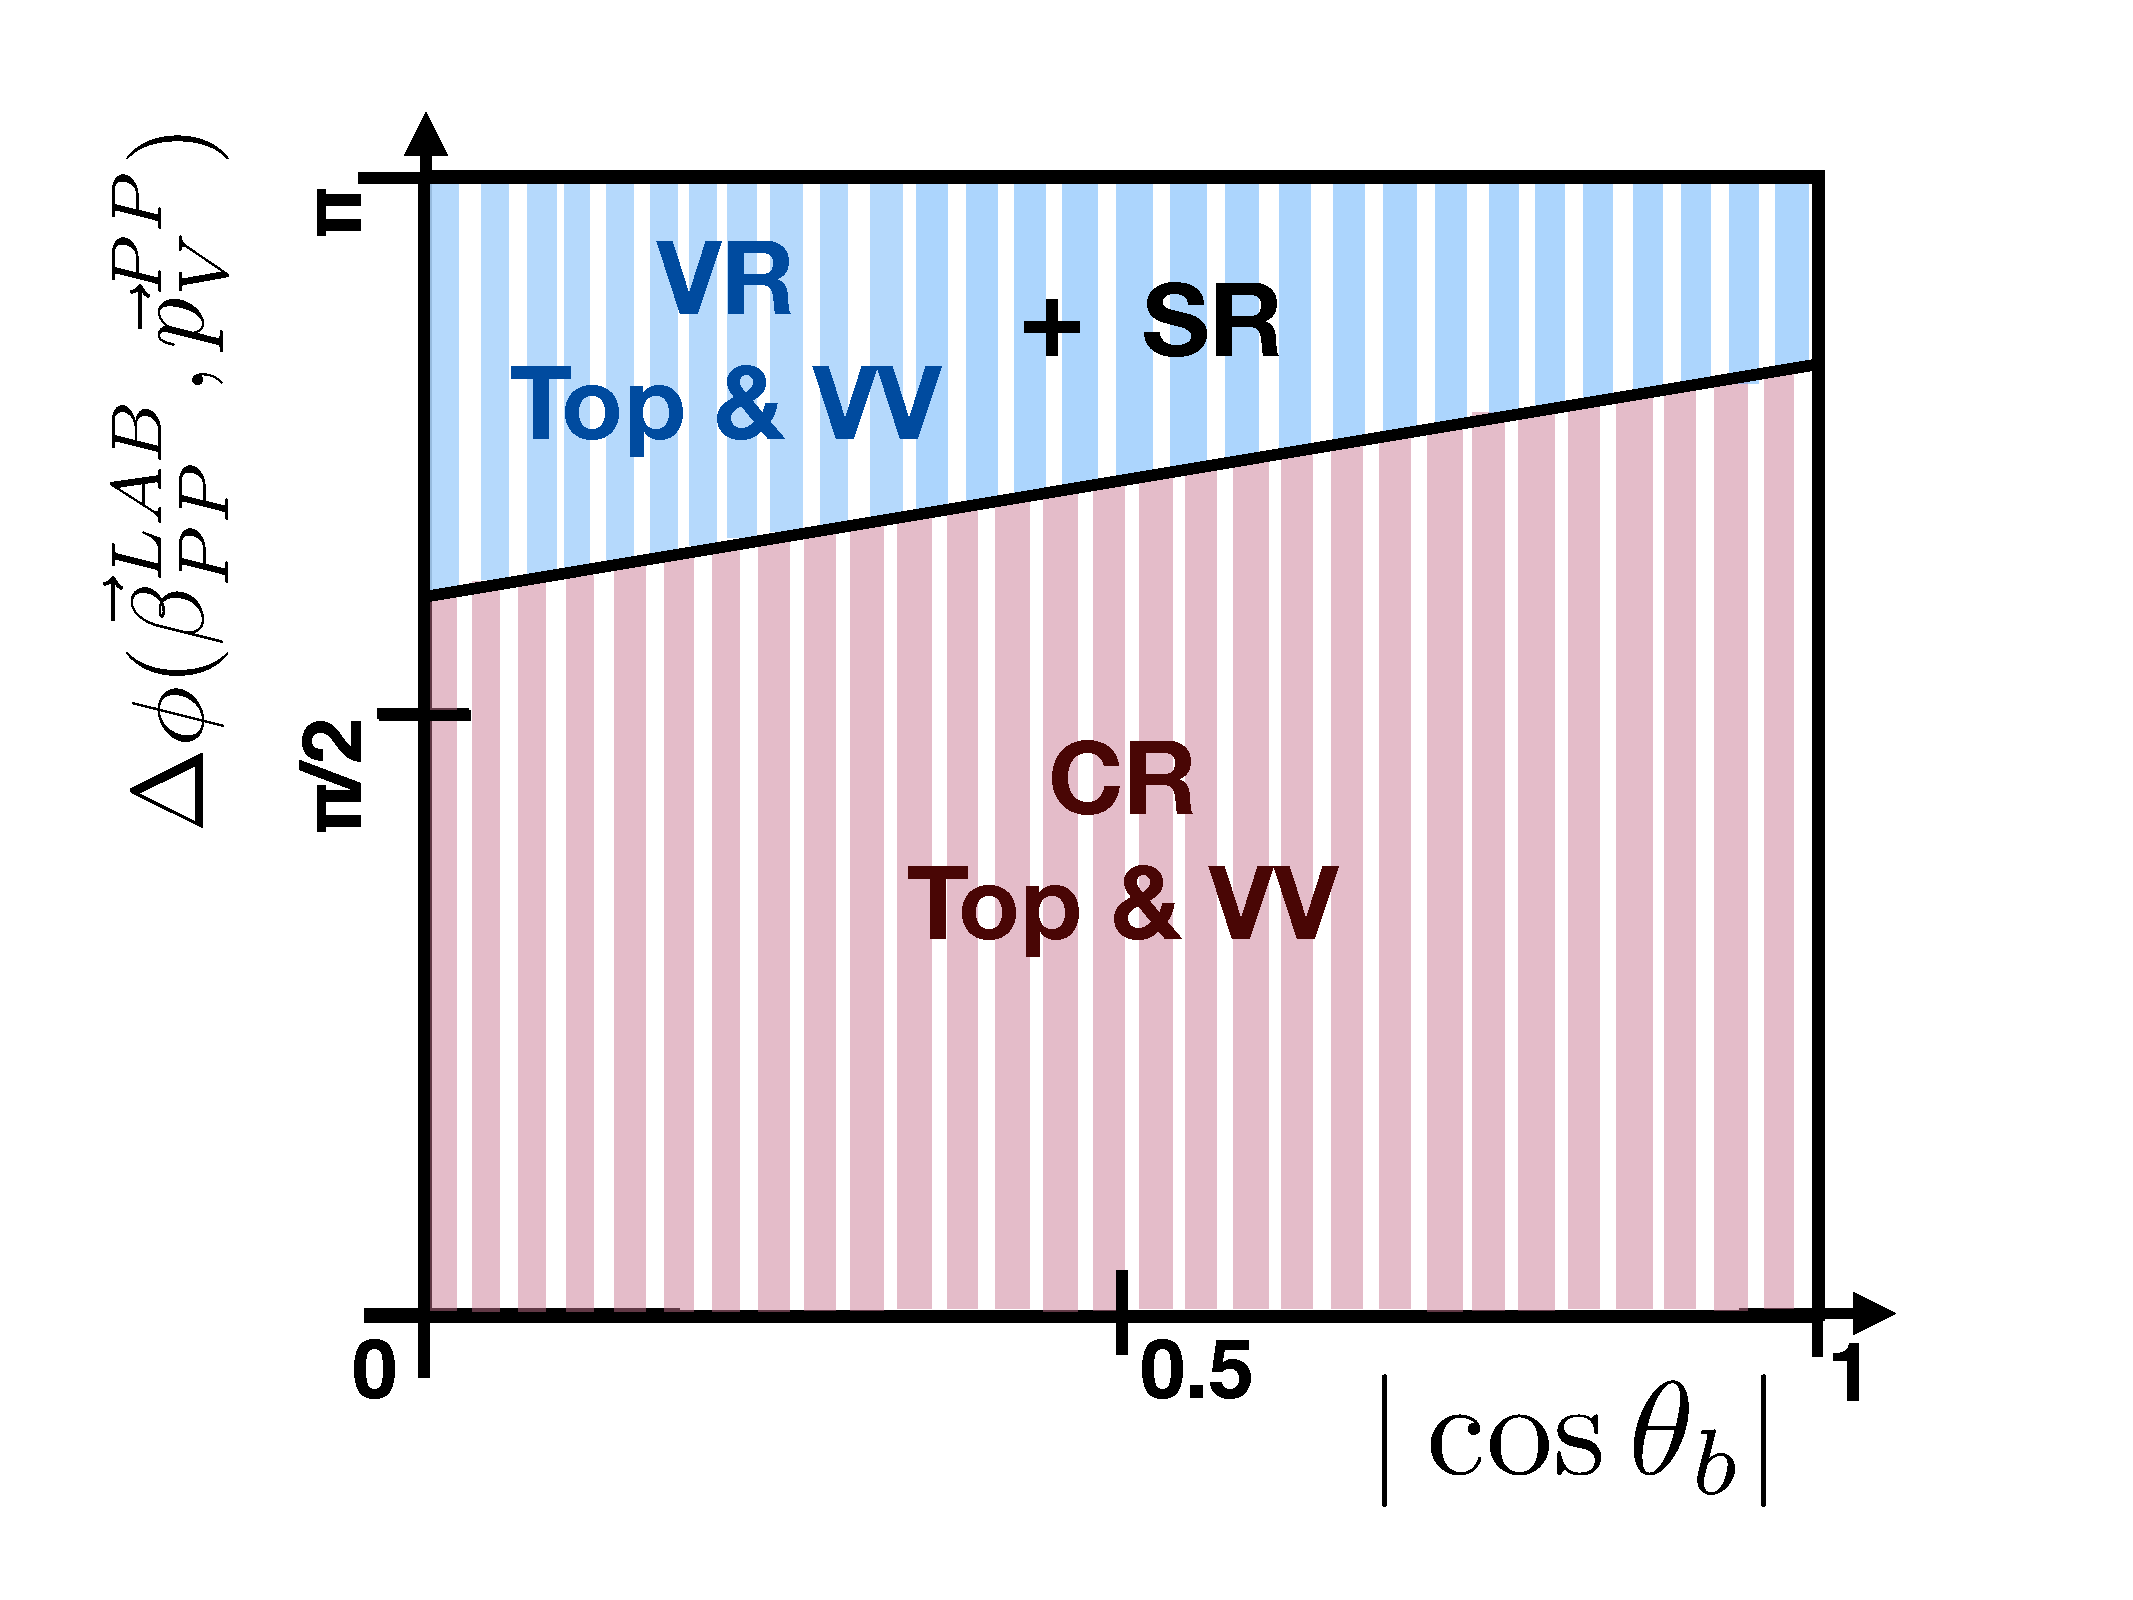
\includegraphics[width=0.7\textwidth]{figures/search_stop2l/bkg_est/crvrmotivation}
        \caption{
            Illustration of the CR and VR strategy used in the \bWN search.
            The defining characteristic for the definition of these regions is
            based on the region in the $(\cosb, \dpb)$-plane that they select.
            The CR inverts the requirements on these quantities relative to the SRs,
            while the VR has the same requirements as in the SRs but inverts
            selections made on the other observables.
        }
        \label{fig:stop_crvr_motivation}
    \end{center}
\end{figure}

%%%%%%%%%%%%%%%%%%%%%%%%%%%%%%%%%%%%%%%%%%%%%%%%%%%%%%%%%%%%%%%%%%%%%%%%%%%%%%%%%%%%%%%%%%%%
%%%%%%%%%%%%%%%%%%%%%%%%%%%%%%%%%%%%%%%%%%%%%%%%%%%%%%%%%%%%%%%%%%%%%%%%%%%%%%%%%%%%%%%%%%%%
%%%%%%%%%%%%%%%%%%%%%%%%%%%%%%%%%%%%%%%%%%%%%%%%%%%%%%%%%%%%%%%%%%%%%%%%%%%%%%%%%%%%%%%%%%%%
%
% TOP BKG
%
%%%%%%%%%%%%%%%%%%%%%%%%%%%%%%%%%%%%%%%%%%%%%%%%%%%%%%%%%%%%%%%%%%%%%%%%%%%%%%%%%%%%%%%%%%%%
%%%%%%%%%%%%%%%%%%%%%%%%%%%%%%%%%%%%%%%%%%%%%%%%%%%%%%%%%%%%%%%%%%%%%%%%%%%%%%%%%%%%%%%%%%%%
%%%%%%%%%%%%%%%%%%%%%%%%%%%%%%%%%%%%%%%%%%%%%%%%%%%%%%%%%%%%%%%%%%%%%%%%%%%%%%%%%%%%%%%%%%%%

\subsection{Top-quark pair production}
\label{sec:stop_ttbar_estimate}

The CRs and VRs designed to derive and validate the semi-data-driven
normalisation correction factor for the \ttbar~background process are called
CR-Top and VR-Top, respectively, and are defined in Table~\ref{tab:stop_top_crvr}.
The strategy for the CR and VR selections in the $(\cosb, \dpb)$ plane are described
in the previous section.
Several of the selections on the kinematic quantities relative to those in the SRs (c.f. Table~\ref{tab:stop_sr_def})
are relaxed.
In both CR-Top and VR-Top, the \mdr requirement is relaxed to $\mdr > 80$\,GeV and the requirement on the
\gaminv quantity is removed.
In VR-Top, the \rpt requirement is inverted relative to that used in the SRs.
Given that the \ttbar~background is flavor symmetric, only different-flavor events
are allowed to populate CR-Top and VR-Top, in order to avoid contamination from $Z$-boson processes.
As a result, no additioanl requirement on $m_{\ell\ell}$ is made in these regions.
For increased purity, CR-Top requires that there be at least one $b$-tagged jet,
while VR-Top applies a veto in order to be orthogonal to CR-Top.

VR-Top is defined to have zero $b$-tagged jets, while CR-Top requires at least one.
In dedicated studies, it has been verified that the \ttbar~normalisation correction derived
in the $b$-jet rich region CR-Top is well extrapolated to separate validation regions, and is rather
independent of the $b$-tagged jet multiplicity.
This gives confidence that VR-Top can be used as an appropriate check on the \ttbar~normalisation
correct factor and that it's extrapolation to the SRs, which have differing requirements on the
$b$-tagged jet multiplicity, is reasonable.

\begin{table}[!htb]
    \begin{center}
        \caption{
            Definitions of the CR and VR for the \ttbar~background process for the
            \bWN search.
        }
        \label{tab:stop_top_crvr}
        \begin{tabular}{l | c c}
            \hline
            \hline
                & \multicolumn{2}{c}{\textbf{Regions}} \\
            \hline
            \textbf{Variable} & \textbf{CR-Top} & \textbf{VR-Top} \\
            \hline
            Dilepton Flavor & \multicolumn{2}{c}{DF} \\
            $m_{\ell\ell}$ [GeV]    & \multicolumn{2}{c}{no req.} \\
            Lead lepton \pT~[GeV] & \multicolumn{2}{c}{$>25$} \\
            Sub-lead lepton \pT~[GeV] & \multicolumn{2}{c}{$>20$} \\
            $b$-tagged jet multiplicity & $>0$ & Exactly 0 \\
            \mdr [GeV] & \multicolumn{2}{c}{$>80$} \\
            \rpt & $>0.7$ & $<0.7$ \\
            \gaminv & \multicolumn{2}{c}{no req.} \\
            $(\cosb, \dpb)$ & $\dpb $ & $\dpb$ \\
                    & \hspace{1.8cm} $< 0.9 \times | \cosb | + 1.6$ & \hspace{1.8cm}$> 0.9 \times | \cosb | + 1.6$ \\
            \hline
            \hline
        \end{tabular}
    \end{center}
\end{table}

\subsubsection{Kinematic Distributions in CR-Top}

\begin{figure}[!htb]
    \begin{center}
        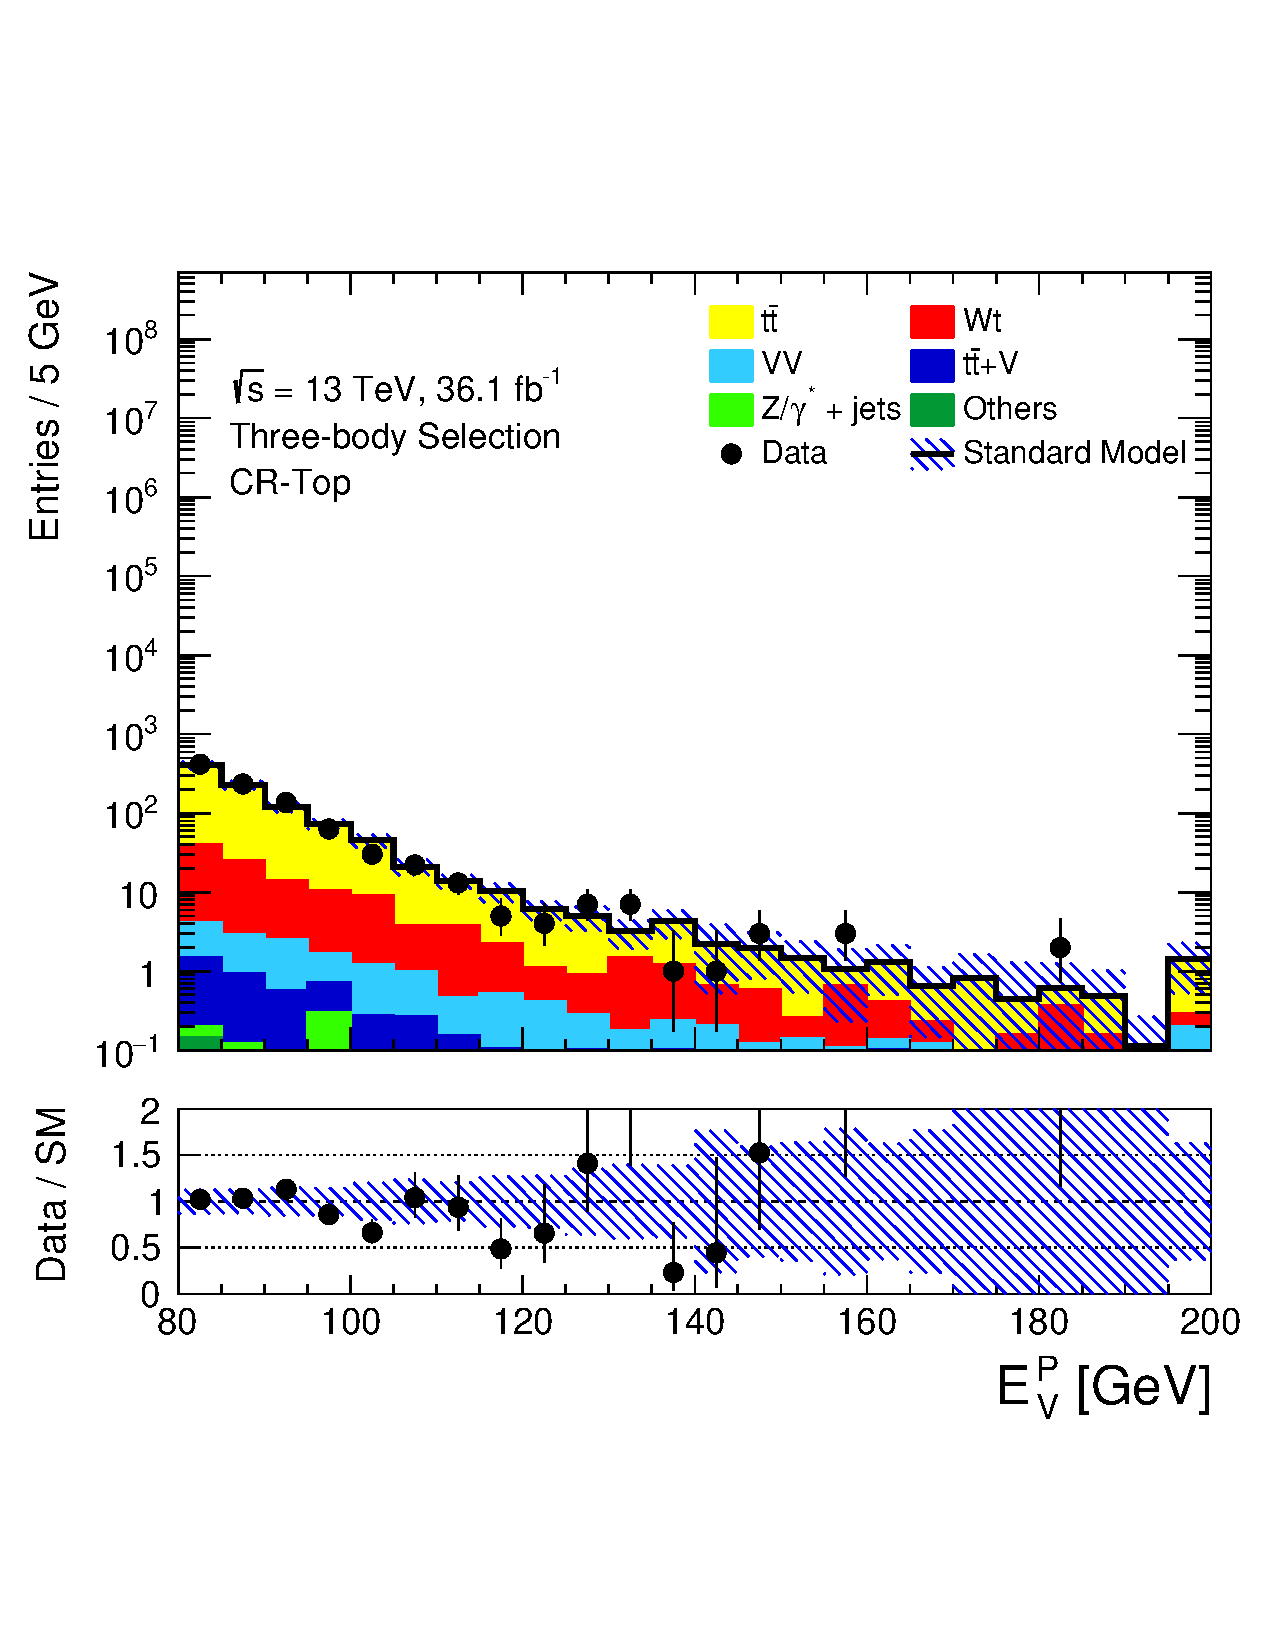
\includegraphics[width=0.48\textwidth]{figures/search_stop2l/bkg_est/crtop/crt_MDR}
    \end{center}
\end{figure}



%%%%%%%%%%%%%%%%%%%%%%%%%%%%%%%%%%%%%%%%%%%%%%%%%%%%%%%%%%%%%%%%%%%%%%%%%%%%%%%%%%%%%%%%%%%%
%%%%%%%%%%%%%%%%%%%%%%%%%%%%%%%%%%%%%%%%%%%%%%%%%%%%%%%%%%%%%%%%%%%%%%%%%%%%%%%%%%%%%%%%%%%%
%%%%%%%%%%%%%%%%%%%%%%%%%%%%%%%%%%%%%%%%%%%%%%%%%%%%%%%%%%%%%%%%%%%%%%%%%%%%%%%%%%%%%%%%%%%%
%
% VV BKG
%
%%%%%%%%%%%%%%%%%%%%%%%%%%%%%%%%%%%%%%%%%%%%%%%%%%%%%%%%%%%%%%%%%%%%%%%%%%%%%%%%%%%%%%%%%%%%
%%%%%%%%%%%%%%%%%%%%%%%%%%%%%%%%%%%%%%%%%%%%%%%%%%%%%%%%%%%%%%%%%%%%%%%%%%%%%%%%%%%%%%%%%%%%
%%%%%%%%%%%%%%%%%%%%%%%%%%%%%%%%%%%%%%%%%%%%%%%%%%%%%%%%%%%%%%%%%%%%%%%%%%%%%%%%%%%%%%%%%%%%

\subsection{Diboson Production}
\label{sec:stop_vv_estimate}

\begin{table}[!htb]
    \begin{center}
        \caption{
            Definitions of the CR and VR for the diboson~background processes for the
            \bWN search.
        }
        \begin{tabular}{l | c c c c}
            \hline
            \hline
                & \multicolumn{4}{c}{\textbf{Regions}} \\
            \hline
            \textbf{Variable} & \textbf{CR-VV-DF} & \textbf{CR-VV-SF} & \textbf{VR-VV-DF} & \textbf{VR-VV-SF} \\
            \hline
            Dilepton Flavor & DF & SF & DF & SF \\
            $m_{\ell\ell}$ [GeV]    & no req. & $|m_{\ell\ell} - 91.2| > 10$ & no req. & $|m_{\ell\ell} - 91.2| > 10$ \\
            Lead lepton \pT~[GeV] & $>25$ & $>25$ & $>25$ & $>25$ \\
            Sub-lead lepton \pT~[GeV] & $>20$ & $>20$ & $>20$ & $>20$ \\
            $b$-tagged jet multiplicity & Exactly 0 & Exactly 0 & Exactly 0 & Exactly 0 \\
            \mdr [GeV] & $>50$ & $>70$ & $\in(50,95)$ & $\in(60,95)$ \\
            \rpt & $<0.5$ & $<0.5$ & $<0.7$ & $<0.4$ \\
            \gaminv &  $>0.7$ & $>0.7$ & $>0.7$ & $>0.7$ \\
            $(\cosb, \dpb)$ & \multicolumn{2}{c}{\small{$\dpb < 0.9 \times | \cosb | + 1.6$}} & \multicolumn{2}{c}{\small{$\dpb> 0.9 \times | \cosb | + 1.6$}} \\
%            $(\cosb, \dpb)$ & $\dpb $  &  $\dpb$ & \\
%                    & \hspace{1.8cm} $< 0.9 \times | \cosb | + 1.6$  & \hspace{1.8cm}$> 0.9 \times | \cosb | + 1.6$ \\
            \hline
            \hline
        \end{tabular}
    \end{center}
\end{table}

%%%%%%%%%%%%%%%%%%%%%%%%%%%%%%%%%%%%%%%%%%%%%%%%%%%%%%%%%%%%%%%%%%%%%%%%%%%%%%%%%%%%%%%%%%%%
%%%%%%%%%%%%%%%%%%%%%%%%%%%%%%%%%%%%%%%%%%%%%%%%%%%%%%%%%%%%%%%%%%%%%%%%%%%%%%%%%%%%%%%%%%%%
%%%%%%%%%%%%%%%%%%%%%%%%%%%%%%%%%%%%%%%%%%%%%%%%%%%%%%%%%%%%%%%%%%%%%%%%%%%%%%%%%%%%%%%%%%%%
%
% POST FIT
%
%%%%%%%%%%%%%%%%%%%%%%%%%%%%%%%%%%%%%%%%%%%%%%%%%%%%%%%%%%%%%%%%%%%%%%%%%%%%%%%%%%%%%%%%%%%%
%%%%%%%%%%%%%%%%%%%%%%%%%%%%%%%%%%%%%%%%%%%%%%%%%%%%%%%%%%%%%%%%%%%%%%%%%%%%%%%%%%%%%%%%%%%%
%%%%%%%%%%%%%%%%%%%%%%%%%%%%%%%%%%%%%%%%%%%%%%%%%%%%%%%%%%%%%%%%%%%%%%%%%%%%%%%%%%%%%%%%%%%%

\begin{table}[!htb]
\begin{center}
\setlength{\tabcolsep}{0.0pc}
{\scriptsize
\caption{
Yields in the \ttbar~and diboson CRs and VRs for the \bWN search for the main background processes
contributing to the analysis.
The lower-portion of the table are the yields before the background-only fit to data
in the CRs, without the normalisation corrections applied.
The upper-portion of the table are those taken after the background-only fit to data.
The errors on the quoted numbers are due to the statistical and experimental systematic uncertainties.
}
\label{tab:bkgonly_CRVR}
\begin{tabular*}{\textwidth}{@{\extracolsep{\fill}}lrrrrrr}
\noalign{\smallskip}\hline\noalign{\smallskip}
\noalign{\smallskip}\hline\noalign{\smallskip}
\textbf{Process}           & \textbf{CR-Top}            & \textbf{CR-VV-DF}            & \textbf{CR-VV-SF}            & \textbf{VR-Top}           & \textbf{VR-VV-DF}            & \textbf{VR-VV-SF}              \\[-0.05cm]
\noalign{\smallskip}\hline\noalign{\smallskip}


Observed Data         & $951$              & $2046$              & $1275$              & $1197$              & $1896$              & $783$                    \\
\noalign{\smallskip}\hline\noalign{\smallskip}
%%
Post-fit Total SM         & $951.00 \pm 30.84$          & $2046.05 \pm 45.23$          & $1275.17 \pm 35.68$          & $1231.78 \pm 86.59$          & $2013.57 \pm 116.49$          & $780.44 \pm 117.32$              \\
\noalign{\smallskip}\hline\noalign{\smallskip}
%%
        Post-fit \ttbar          & $833.03 \pm 32.85$          & $619.74 \pm 111.40$          & $333.62 \pm 60.91$          & $733.87 \pm 64.91$          & $754.94 \pm 78.17$          & $127.14 \pm 22.09$              \\
%%
        Post-fit Diboson (DF)          & $11.51 \pm 2.43$          & $1093.28 \pm 125.83$          & $0.00 \pm 0.00$          & $331.13 \pm 82.57$          & $886.53 \pm 168.16$          & $0.00 \pm 0.00$              \\
%%
        Post-fit Diboson (SF)          & $0.00 \pm 0.00$          & $0.00 \pm 0.00$          & $378.94 \pm 124.32$          & $0.00 \pm 0.00$          & $0.00 \pm 0.00$          & $380.00 \pm 141.58$              \\
%%
        Post-fit Single-top          & $101.10 \pm 9.73$          & $186.47 \pm 27.99$          & $103.47 \pm 17.43$          & $111.52 \pm 14.49$          & $151.88 \pm 14.37$          & $36.40 \pm 5.62$              \\
%%
        Post-fit $\ttbar+V$          & $4.35 \pm 0.42$          & $0.39 \pm 0.07$          & $0.36 \pm 0.07$          & $1.27 \pm 0.22$          & $0.42 \pm 0.13$          & $0.05 \pm 0.02$              \\
%%
        Post-fit $Z$+jets          & $0.70 \pm 0.22$          & $1.83_{-1.83}^{+2.55}$          & $428.58 \pm 92.55$          & $0.47_{-0.47}^{+0.85}$          & $0.39_{-0.39}^{+0.71}$          & $191.37 \pm 78.38$              \\
%%
        Post-fit Single-higgs          & $0.31 \pm 0.13$          & $78.95 \pm 9.17$          & $6.23 \pm 1.06$          & $0.44_{-0.44}^{+0.52}$          & $54.98 \pm 4.34$          & $9.40 \pm 1.11$              \\
%%
        Post-fit Fakes          & $0.00 \pm 0.00$          & $65.37 \pm 2.22$          & $23.96 \pm 1.25$          & $53.09 \pm 1.92$          & $164.42 \pm 5.68$          & $36.09 \pm 3.04$              \\
%%
 \noalign{\smallskip}\hline\noalign{\smallskip}
%%
 Total SM               & $905.14 \pm 16.54$          & $1988.38 \pm 110.43$          & $1248.21 \pm 123.42$          & $1184.39 \pm 71.23$          & $1952.92 \pm 61.72$          & $764.65 \pm 99.06$              \\
\noalign{\smallskip}\hline\noalign{\smallskip}
%%
         \ttbar          & $787.43 \pm 11.29$          & $585.87 \pm 102.00$          & $315.39 \pm 55.87$          & $693.71 \pm 53.51$          & $713.64 \pm 66.57$          & $120.19 \pm 20.17$              \\
%%
         Diboson (DF)          & $11.25 \pm 1.62$          & $1069.46 \pm 12.45$          & $0.00 \pm 0.00$          & $323.89 \pm 50.27$          & $867.18 \pm 77.75$          & $0.00 \pm 0.00$              \\
%%
         Diboson (SF)          & $0.00 \pm 0.00$          & $0.00 \pm 0.00$          & $370.13 \pm 15.48$          & $0.00 \pm 0.00$          & $0.00 \pm 0.00$          & $371.16 \pm 34.38$              \\
%%
         Single-top          & $101.10 \pm 9.80$          & $186.49 \pm 28.25$          & $103.49 \pm 17.59$          & $111.52 \pm 14.60$          & $151.88 \pm 14.46$          & $36.41 \pm 5.66$              \\
%%
         $\ttbar+V$          & $4.35 \pm 0.42$          & $0.39 \pm 0.07$          & $0.36 \pm 0.07$          & $1.27 \pm 0.23$          & $0.42 \pm 0.13$          & $0.05 \pm 0.02$              \\
%%
         $Z$+jets          & $0.70 \pm 0.23$          & $1.83_{-1.83}^{+2.57}$          & $428.65 \pm 93.15$          & $0.48_{-0.48}^{+0.86}$          & $0.40_{-0.40}^{+0.72}$          & $191.36 \pm 78.78$              \\
%%
         Single-higgs          & $0.31 \pm 0.13$          & $78.96 \pm 9.26$          & $6.23 \pm 1.07$          & $0.44_{-0.44}^{+0.53}$          & $54.98 \pm 4.37$          & $9.40 \pm 1.12$              \\
%%
         Fakes          & $0.00 \pm 0.00$          & $65.37 \pm 2.23$          & $23.96 \pm 1.26$          & $53.09 \pm 1.92$          & $164.42 \pm 5.70$          & $36.09 \pm 3.04$              \\
\noalign{\smallskip}\hline\noalign{\smallskip}
\noalign{\smallskip}\hline\noalign{\smallskip}
\end{tabular*}
}
\end{center}
\end{table}

\section{Results}
\label{sec:hh_results}

As with the analysis presented in Chapter~\ref{chap:search_stop}, a profile likelihood
fit is performed, including all CRs and SRs of the analysis and with the observed
data in all regions used as a constraint.
The result of running this fit is shown in Table~\ref{tab:hh_final_sr_yields}.
The observed data and post-fit MC prediction agrees quite well in SR-SF.
In SR-DF there is a slight excess observed in the data relative to the MC prediction.
This excess in SR-DF is not statistically significant however, and amounts to only a $1.05\sigma$ excess
(null $p_0$-value of 0.15).
Figures~\ref{fig:hh_sr_kin_0}-\ref{fig:hh_sr_kin_3} present kinematic distributions comparing
the observed data and post-fit MC prediction for the SM backgrounds in the SR selections.
Figures~\ref{fig:hh_sr_kin_1} and \ref{fig:hh_sr_kin_2} show the \dhh distributions in detail
in SR-DF and SR-SF, respectively.

As there is no significant deviation between the prediction and observed data,
indicating that there is no evidence for enhanced production of Higgs boson pairs, 95\% CL
cross-section upper-limits are derived for the SM-like non-resonant Higgs boson pair
production.
These results are reported in Table~\ref{tab:hh_bbww_xsec_ul} and are with respect to the
$pp \rightarrow hh$ production process, having taken into account the branching ratio for the dilepton $hh \rightarrow \bbww$
decay.
That is, the 95\% CL UL reported in Table~\ref{tab:hh_bbww_xsec_ul} are on \sigmaHH, and not
on $\sigmaHH \times \text{BR}(hh \rightarrow \bbww) \times \text{BR}(WW^* \rightarrow \ell \nu \ell \nu)$.
The effect of the $1.05\sigma$ excess in SR-DF is seen in the observed 95\% CL UL, which in Table~\ref{tab:hh_bbww_xsec_ul}
is seen to be larger than the expected value by roughly $1\sigma$.
Figure~\ref{fig:hh_ul_comp} illustrates the results listed in Table~\ref{tab:hh_bbww_xsec_ul},
while also comparing them to the leading $hh$ searches (c.f. Figure~\ref{fig:hh_comb_36}): $hh \rightarrow \bbbb$,
$hh \rightarrow \bbtautau$, and $hh \rightarrow \bbyy$.
The comparisons with the other analyses are made only with respect to the expected 95\% CL cross-section upper-limits.
It should be remembered that the other analyses in Figure~\ref{fig:hh_comb_36} are based only on the partial Run 2
dataset, collected in 2015--2016 and comprised of $36.2$\,fb$^{-1}$ of $pp$ collision data.
However, the analysis presented in this chapter is the first time that this search has been performed
in ATLAS and it is already improving the prospects of searches for $hh$ in the \bbww channel by roughly
a factor of 10 (c.f. Figure~\ref{fig:hh_comb_36}).
%At the time of writing, work has already started with the aim of improving the results presented here.
One such improvement, based on performing a multi-binned shape analysis wherein the full \textit{shape} of the \dhh
distribution is used as input to the hypothesis tests --- as opposed to simply \textit{cutting} on the \dhh distribution
and defining simple signal regions as in Table~\ref{tab:hh_sr_def} --- is expected to increase the sensitivity to the $hh \rightarrow \bbww$ signal process
substantially.

One question that the searches for Higgs boson pair production should being thinking about,
as they start preparing for the time when they begin to make observation of Higgs boson pairs,
is whether or not they are designed in such a way as to make meaningful statements about the
Higgs self-coupling parameter, $\lambda$.
As shown in Figure~\ref{fig:hh_feynman}, the leading contributions to Higgs boson pair production
at the LHC proceeds via two diagrams, only one of which is sensitive to $\lambda$.
The final state kinematics resulting from Higgs bosons originating from the decay of the box-diagram
process tend to be much harder due to the massive top-quark loop being directly coupled to the outgoing Higgs bosons.
As a result, analyses are typically more sensitive to this process as the final state objects are
more directly observable and more efficiently reconstructed.
This is the case for the analysis presented in this chapter, a fact that is illustrated in Figure~\ref{fig:mhh_sel_eff}.
The $hh$ system invariant mass in the box-diagram decays
tends to be larger than that of the triangle diagram.
An indication, then, of whether an analysis is tuned to be sensitive to decays relevant
for the measurement of $\lambda$ is whether or not they are sensitive to the lower portion of the $m_{hh}$ distribution.
From Figure~\ref{fig:mhh_sel_eff}, it is clear that the present analysis is more sensitive to the decays from the box-diagram.
Given the early stages of the $hh$ search program in ATLAS, however, this is not currently
an urgent issue.
The preliminary aim for the $hh$ search program has been to define exactly which channels will be effective
at observing $hh$ signal events, in general, and to design analyses that can optimally search
for the many potential sources of \textit{enhanced} Higgs boson pair production.
As the searches become sensitive to the $hh$ production process, as predicted in the SM,
the next steps will be to understand how to design the analyses such that they maximally
discriminate between the box-type and triangle-type kinematics so as to improve the overall prospects
for the measurement of the Higgs self-coupling parameter.

\begin{table}[!htb]
    \begin{center}
        \caption{
            Observed and predicted yields in the SRs for the dilepton $hh \rightarrow \bbww$ search.
        }
        \label{tab:hh_final_sr_yields}
        \begin{tabular}{l | c c}
        \hline
        \hline
                & \multicolumn{2}{c}{\textbf{Regions}} \\
            \cline{2-3}
            \textbf{Process} & \textbf{SR-SF} & \textbf{SR-DF} \\
            \hline
            Observed Data   & 16 & 9 \\
            \hline
            Post-fit Total SM & $14.88 \pm 2.12$ & $4.88 \pm 1.24$ \\
            \hline
            Post-fit \ttbar & $2.57 \pm 0.97$ & $1.74 \pm 0.66$ \\
            Post-fit Single-top $Wt$ & $2.27 \pm 0.54$ & $2.04 \pm 0.64$ \\
            Post-fit $Z$+heavy-flavor & $7.76 \pm 1.04$ & $0.21 \pm 0.05$ \\
            \hline
            SM & $14.12 \pm 2.05$ & $5.83 \pm 1.42$ \\
            \hline
            \ttbar & $3.26 \pm 1.17$ & $2.20 \pm 0.80$ \\
            Single-top $Wt$ & $2.88 \pm 0.59$ & $2.58 \pm 0.75$ \\
            $\ttbar + V$ & $0.59 \pm 0.07$ & $0.07  \pm 0.06$ \\
            $Z$+heavy-flavor & $5.71 \pm 0.74$ & $0.15 \pm 0.04$ \\
            $Z$+light-flavor & $0.32 \pm 0.14$ & $0.00 \pm 0.00$ \\
            Single-higgs & $0.72 \pm 0.09$ & $0.32 \pm 0.06$ \\
            Fakes & $0.54 \pm 0.38$ & $0.42 \pm 0.36$ \\
        \hline
        \hline
        \end{tabular}
    \end{center}
\end{table}

\begin{table}[!htb]
    \begin{center}
        \caption{
            Expected and observed 95\% CL upper-limits on the Standard Model, non-resonant $hh$
            production cross-section ($\sigma(pp \rightarrow hh)$) and on
            the ratio of the upper-limit on this value to the value predicted in the SM
            ($\sigmaSM = 31.05$ fb).
            The observed limits are in the right most column.
            The $\pm 1 \sigma$ and $\pm 2\sigma$ excursions from the median expected value incorporate the
            effects of the analysis' systematic uncertainties.
        }
        \label{tab:hh_bbww_xsec_ul}
        \begin{tabular}{l | c | c | c | c | c || c }
            \hline
            \hline
                    & $-2\sigma$ & $-1 \sigma$ & \textbf{Median Expected} & $+1 \sigma$ & $+2 \sigma$ & \textbf{Observed} \\
            \hline
                95\% CL UL $\sigma (pp \rightarrow hh)$ [pb] & $0.465$ & $0.641$ & $0.920$ & $1.363$ & $1.990$ & $1.290$ \\
                \sigmaRatio & $14.97$ & $20.66$ & $29.63$ & $43.89$ & $64.02$ & $41.54$ \\
            \hline
            \hline
        \end{tabular}
    \end{center}
\end{table}

%%%%%%%%%%%%%%%%%%%%%%%%%%%%%%%%%%%%%%%%%%%%%%%%%%%%%%%%%%%%%%%%%%%%%%%%%%%%%%%%%%%%%%%%%%%%
%%%%%%%%%%%%%%%%%%%%%%%%%%%%%%%%%%%%%%%%%%%%%%%%%%%%%%%%%%%%%%%%%%%%%%%%%%%%%%%%%%%%%%%%%%%%
%%%%%%%%%%%%%%%%%%%%%%%%%%%%%%%%%%%%%%%%%%%%%%%%%%%%%%%%%%%%%%%%%%%%%%%%%%%%%%%%%%%%%%%%%%%%
%
% SR KIN PLOTS
%
%%%%%%%%%%%%%%%%%%%%%%%%%%%%%%%%%%%%%%%%%%%%%%%%%%%%%%%%%%%%%%%%%%%%%%%%%%%%%%%%%%%%%%%%%%%%
%%%%%%%%%%%%%%%%%%%%%%%%%%%%%%%%%%%%%%%%%%%%%%%%%%%%%%%%%%%%%%%%%%%%%%%%%%%%%%%%%%%%%%%%%%%%
%%%%%%%%%%%%%%%%%%%%%%%%%%%%%%%%%%%%%%%%%%%%%%%%%%%%%%%%%%%%%%%%%%%%%%%%%%%%%%%%%%%%%%%%%%%%

\begin{figure}[!htb]
    \begin{center}
        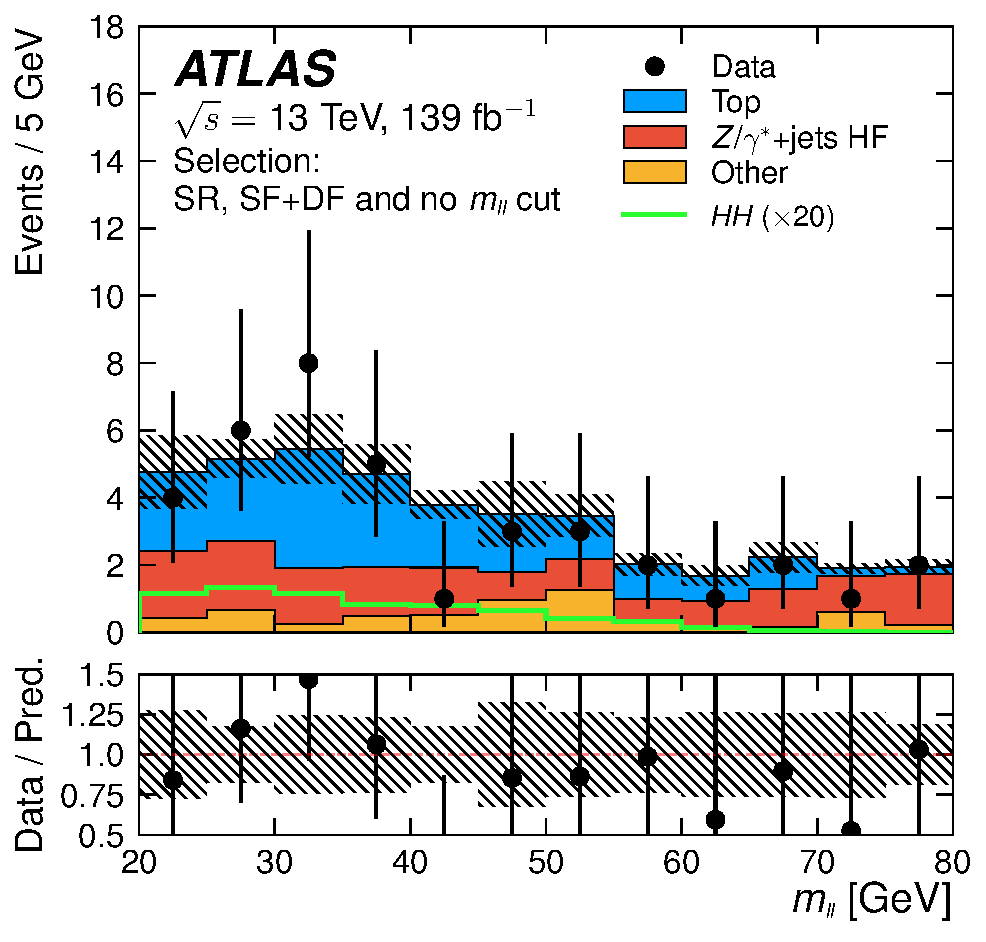
\includegraphics[width=0.48\textwidth]{figures/search_hh/results/sr_plots/srIncNoMllDhh_mll}
        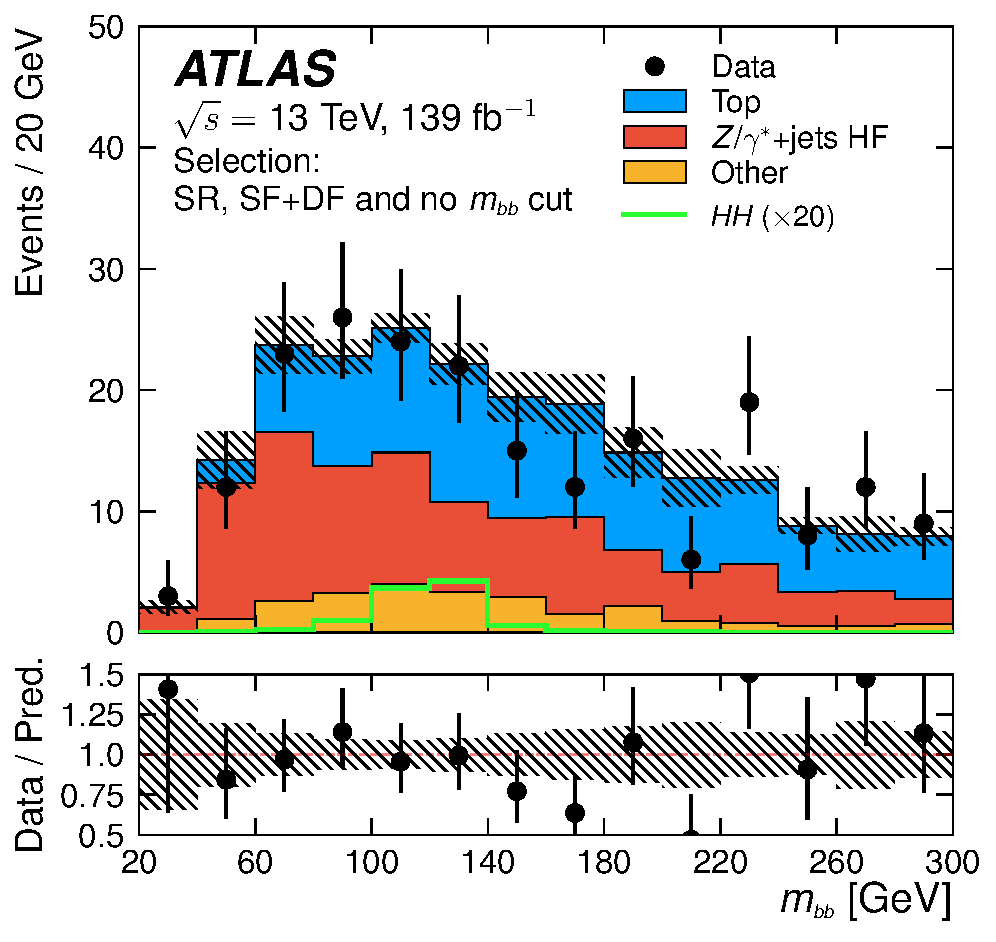
\includegraphics[width=0.48\textwidth]{figures/search_hh/results/sr_plots/srIncNoMbbDhh_mbb}
        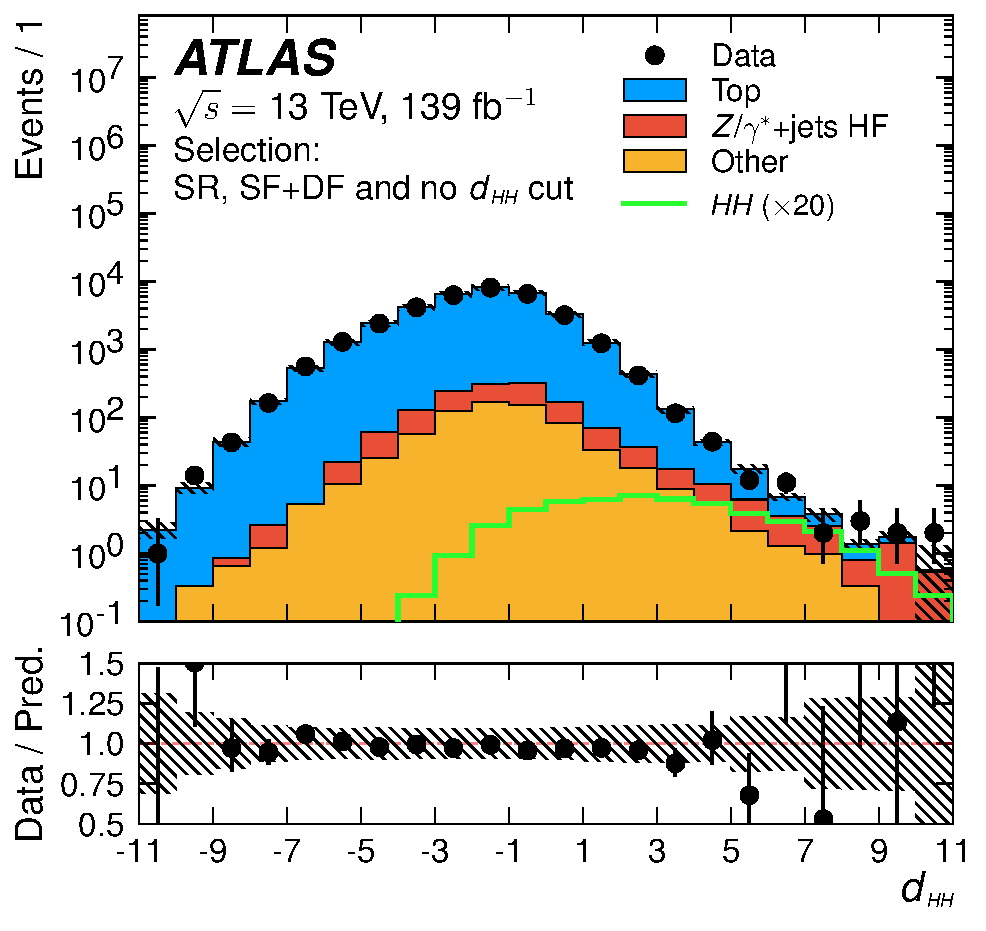
\includegraphics[width=0.48\textwidth]{figures/search_hh/results/sr_plots/srIncNoDhh_NN_d_hh}
        \caption{
            Distributions of $m_{\ell \ell}$ (\textit{\textbf{left}}), $m_{bb}$ (\textit{\textbf{right}}),
            and \dhh (\textit{\textbf{bottom}}).
            The distributions are shown after the fit to data in the control regions under the background-only hypothesis.
            Each distribution includes both the SF and DF events and imposes the analysis SR requirements
            on all quantities except for the one being plotted.
            The SR requirement on \dhh in the $m_{\ell\ell}$ and $m_{bb}$ distributions is relaxed to $\dhh > 5$.
            The dilepton $hh \rightarrow \bbww$ signal, labeled as `$HH$', is shown with its cross-section scaled
            by a factor of 20 relative to the SM prediction for visualization purposes.
            The ratio of the data to the sum of the backgrounds is shown in the lower panel of each figure.
            The hatched bands indicate the combined statistical and systematic uncertainty.
        }
        \label{fig:hh_sr_kin_0}
    \end{center}
\end{figure}

\begin{figure}[!htb]
    \begin{center}
        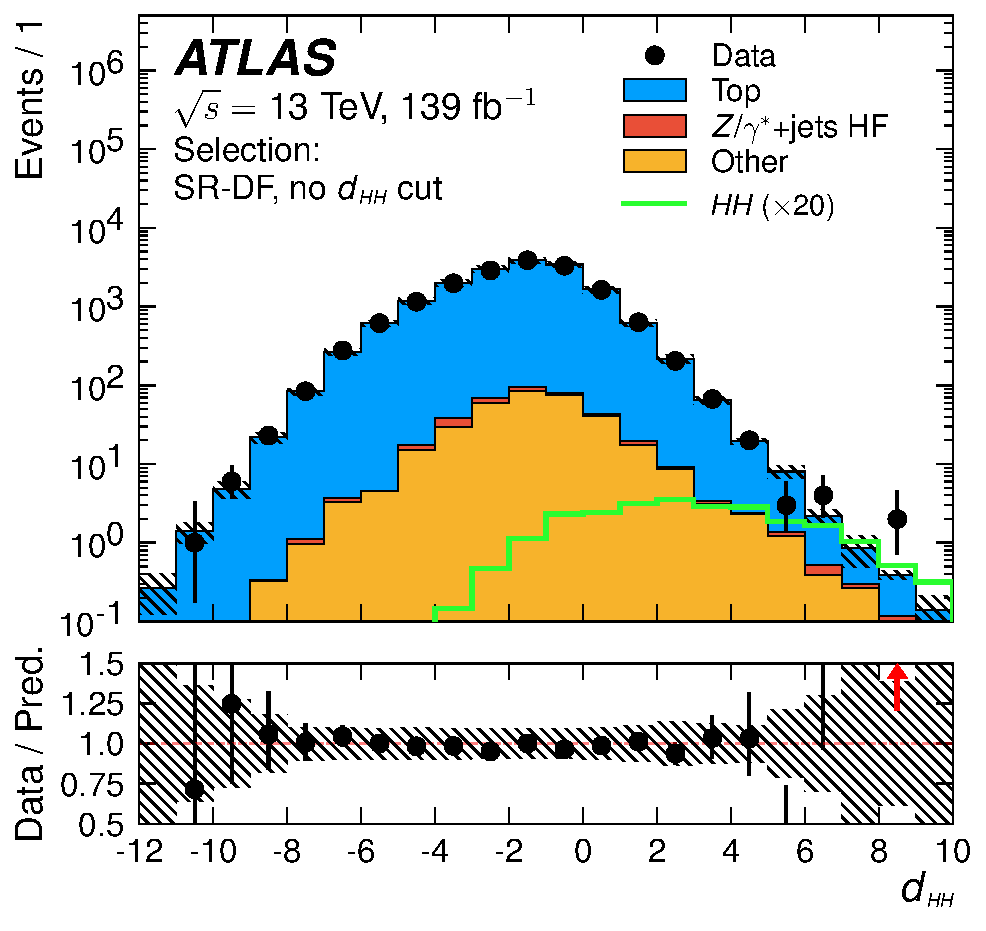
\includegraphics[width=0.48\textwidth]{figures/search_hh/results/sr_plots/srDFNoDhh_NN_d_hh}
        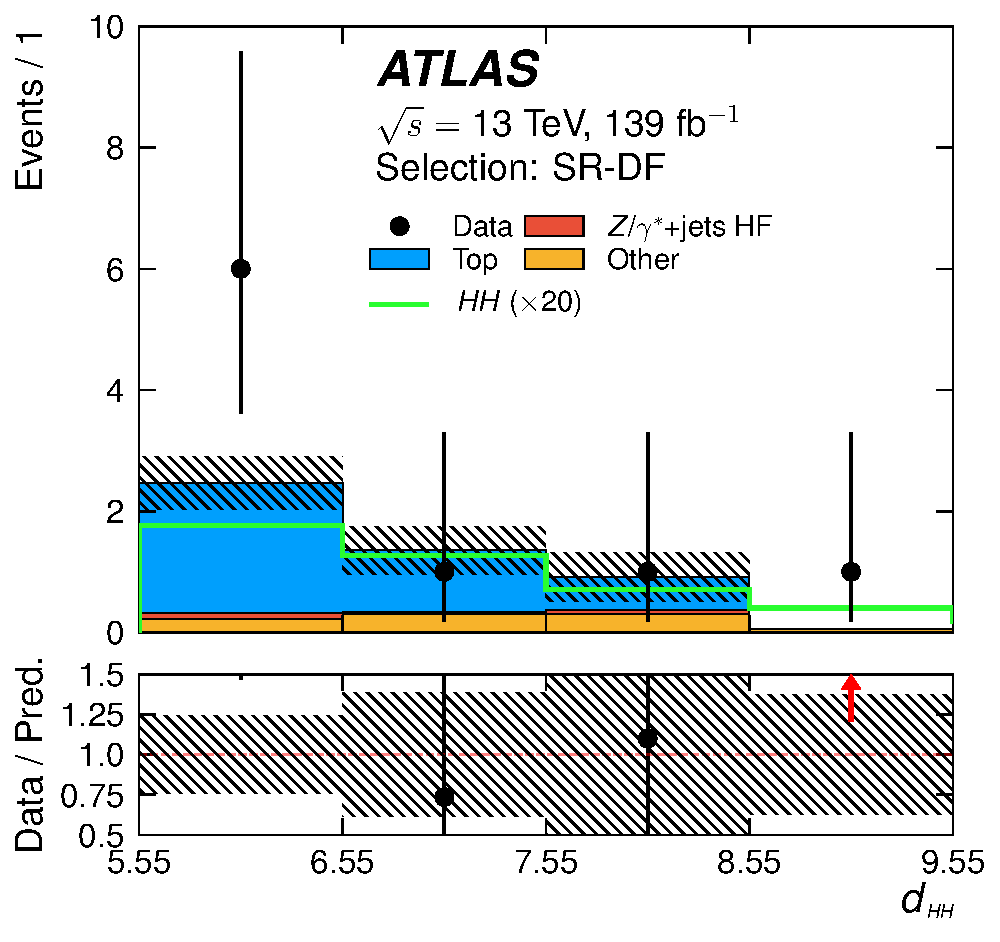
\includegraphics[width=0.48\textwidth]{figures/search_hh/results/sr_plots/srDFNoDhhCloseCut_NN_d_hh}
        \caption{
            Distributions of the \dhh observable in SR-DF without the \dhh selection applied (\textit{\textbf{left}})
            and with the \dhh selection ($\dhh > 5.55$) applied (\textit{\textbf{right}}).
            The dilepton $hh \rightarrow \bbww$ signal, labeled as `$HH$', is shown with its cross-section scaled
            by a factor of 20 relative to the SM prediction for visualization purposes.
            The ratio of the data to the sum of the backgrounds is shown in the lower panel of each figure.
            The hatched bands indicate the combined statistical and systematic uncertainty.
        }
        \label{fig:hh_sr_kin_1}
    \end{center}
\end{figure}
\begin{figure}[!htb]
    \begin{center}
        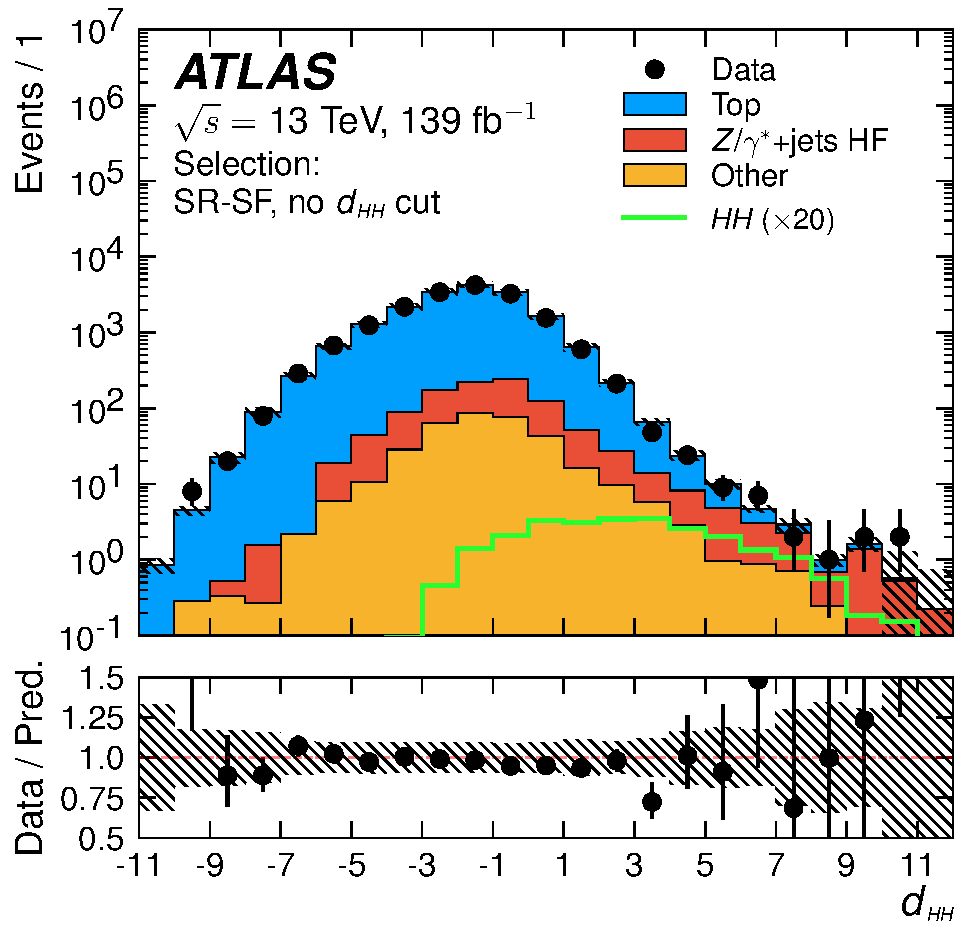
\includegraphics[width=0.48\textwidth]{figures/search_hh/results/sr_plots/srSFNoDhh_NN_d_hh}
        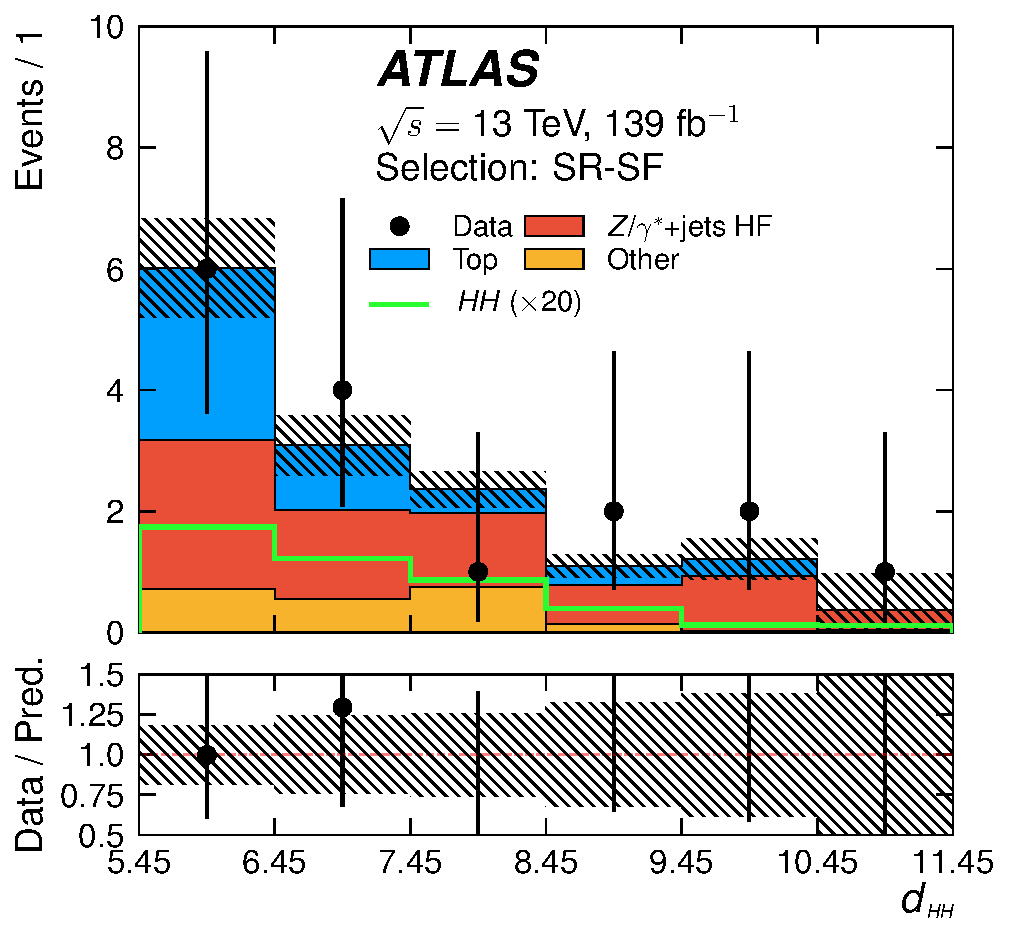
\includegraphics[width=0.48\textwidth]{figures/search_hh/results/sr_plots/srSFNoDhhCloseCut_NN_d_hh}
        \caption{
            Distributions of the \dhh observable in SR-SF without the \dhh selection applied (\textit{\textbf{left}})
            and with the \dhh selection ($\dhh > 5.45$) applied (\textit{\textbf{right}}).
            The dilepton $hh \rightarrow \bbww$ signal, labeled as `$HH$', is shown with its cross-section scaled
            by a factor of 20 relative to the SM prediction for visualization purposes.
            The ratio of the data to the sum of the backgrounds is shown in the lower panel of each figure.
            The hatched bands indicate the combined statistical and systematic uncertainty.
        }
        \label{fig:hh_sr_kin_2}
    \end{center}
\end{figure}

\begin{figure}[!htb]
    \begin{center}
        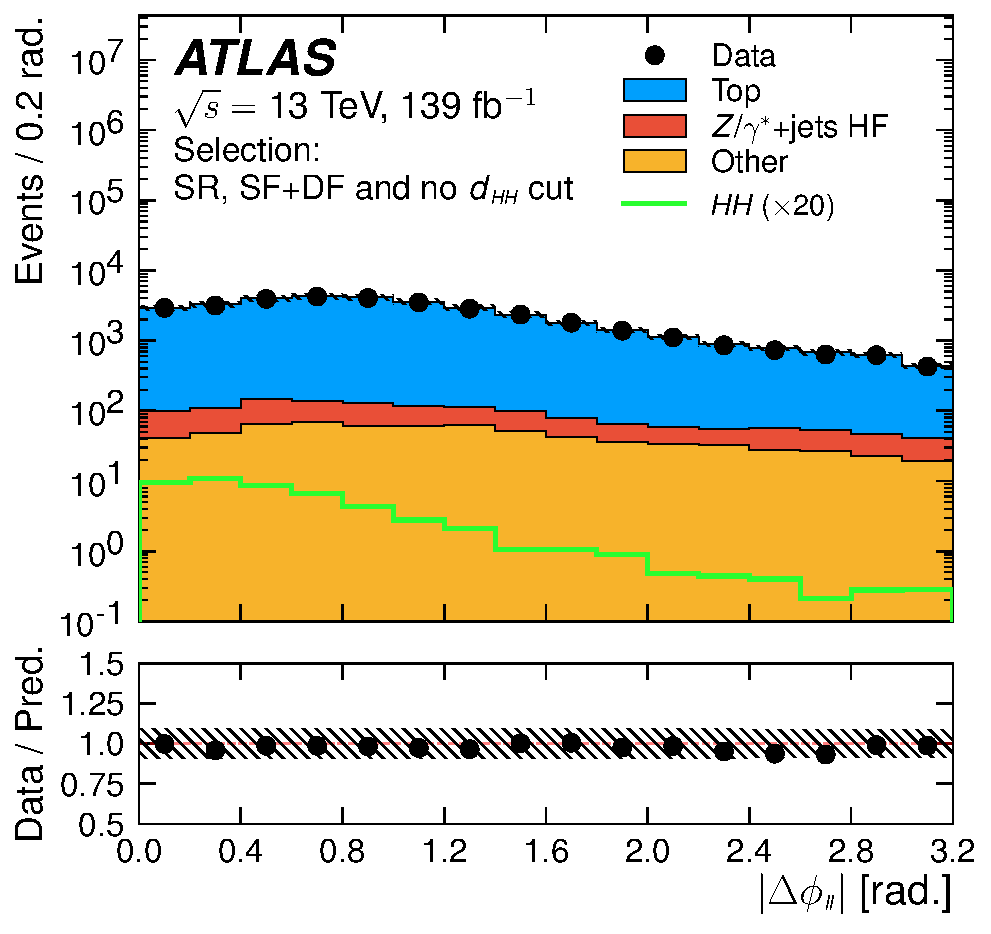
\includegraphics[width=0.48\textwidth]{figures/search_hh/results/sr_plots/srIncNoDhh_dphi_ll}
        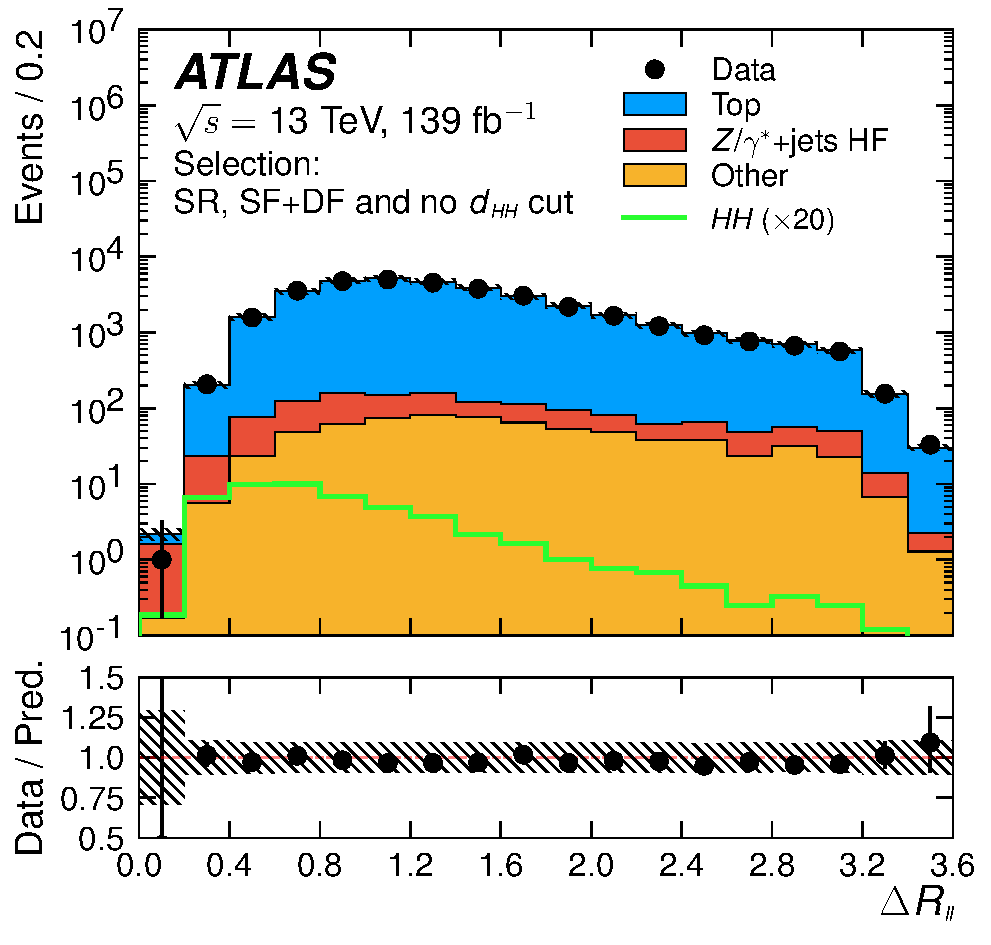
\includegraphics[width=0.48\textwidth]{figures/search_hh/results/sr_plots/srIncNoDhh_dRll}
        \caption{
            Distributions of the $|\dphill|$ and $\drll$ quantities in the analysis' SR selections,
            inclusive of SF and DF dilepton flavors and without the \dhh requirements.
            The dilepton $hh \rightarrow \bbww$ signal, labeled as `$HH$', is shown with its cross-section scaled
            by a factor of 20 relative to the SM prediction for visualization purposes.
            The ratio of the data to the sum of the backgrounds is shown in the lower panel of each figure.
            The hatched bands indicate the combined statistical and systematic uncertainty.
        }
        \label{fig:hh_sr_kin_3}
    \end{center}
\end{figure}

\begin{figure}[!htb]
    \begin{center}
        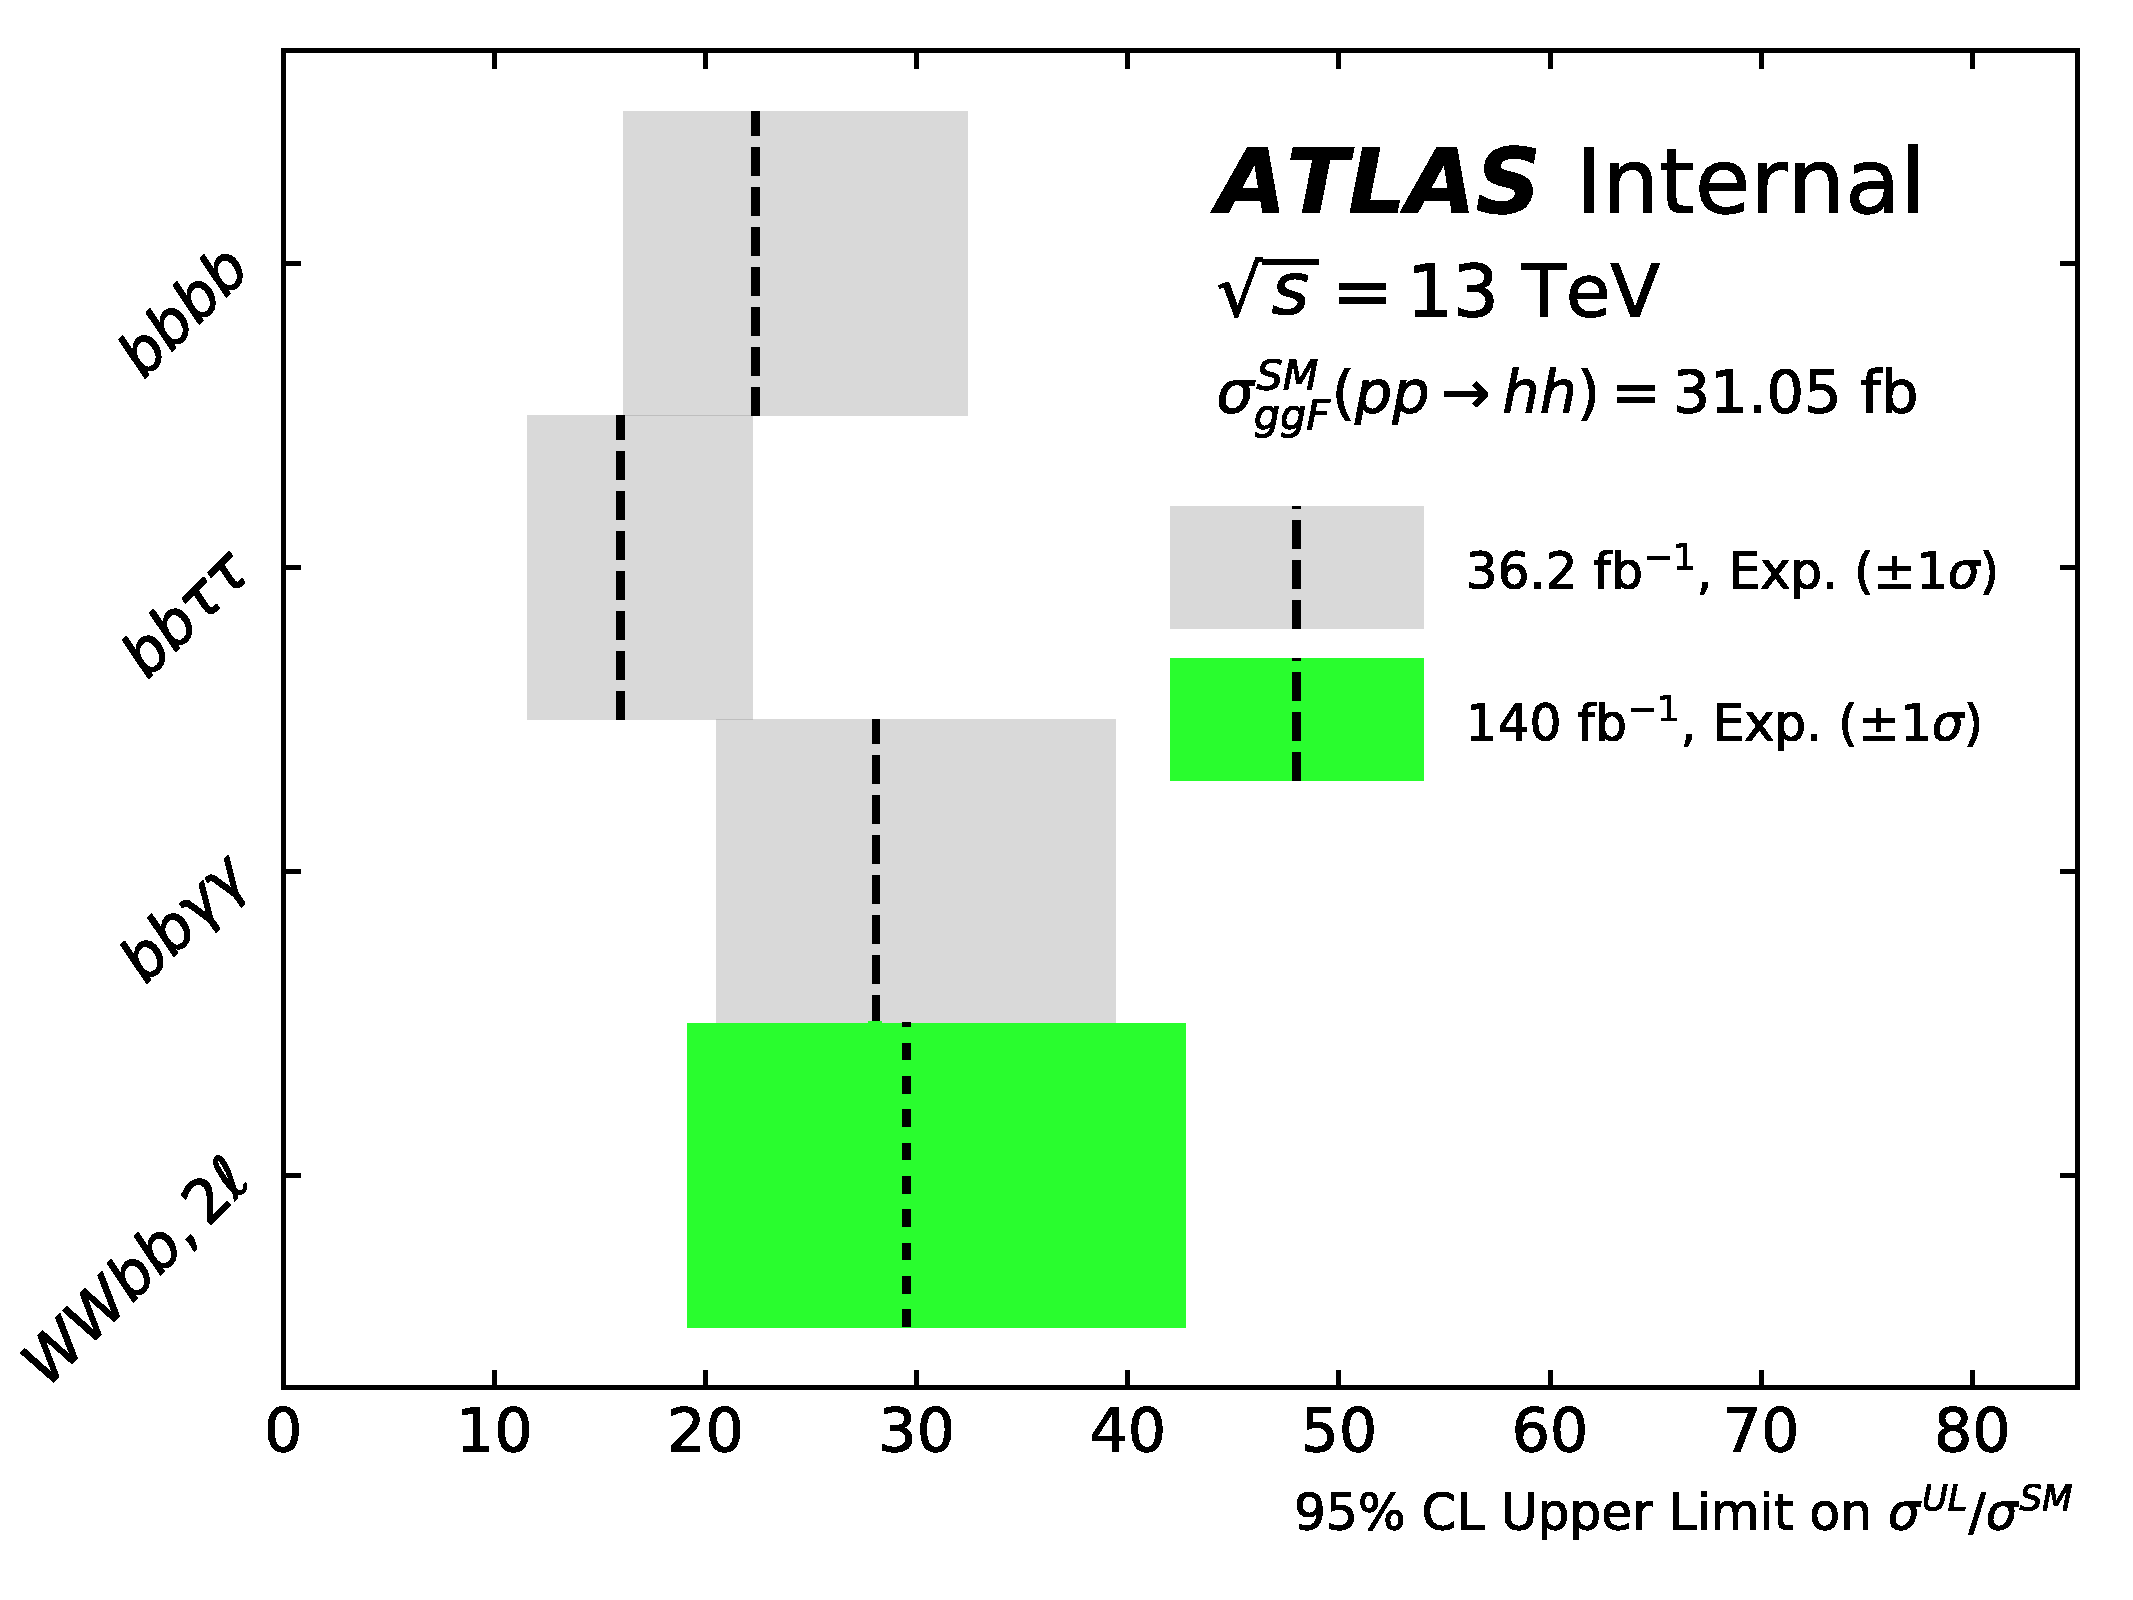
\includegraphics[width=0.6\textwidth]{figures/search_hh/results/hh_ul_compPDF}
        \caption{
            Summary plot showing the $hh$ production cross-section upper limit results, normalized to
            the SM prediction of 31.05\,fb, for the analysis presented in this thesis in green,
            based on the full Run 2 dataset of 139\,fb$^{-1}$ of $pp$ collision data.
            In grey, the partial Run 2 results based on 36\,fb$^{-1}$ of data are shown for comparison.
            Only the expected upper limits are shown.
        }
        \label{fig:hh_ul_comp}
    \end{center}
\end{figure}

\begin{figure}[!htb]
    \begin{center}
        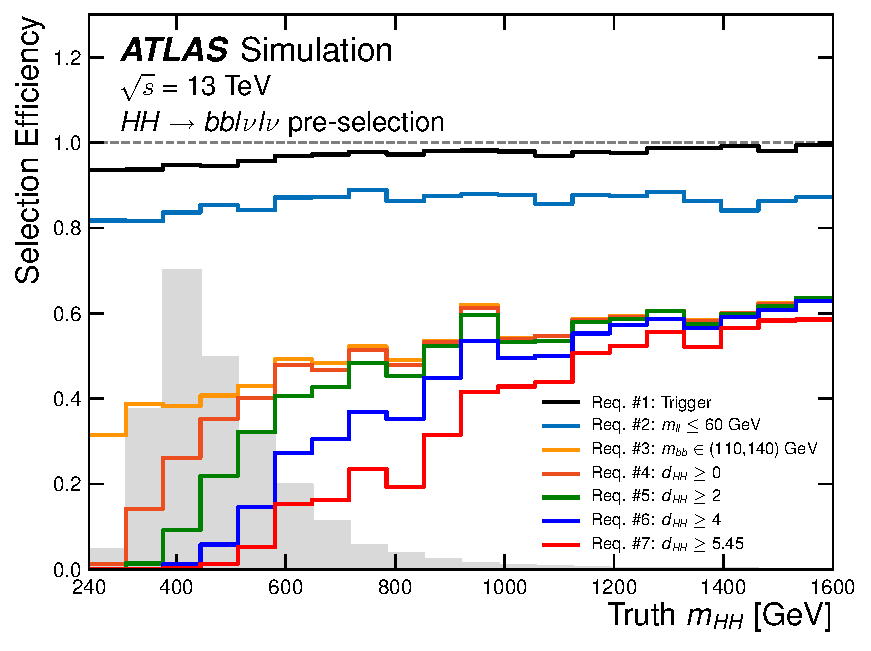
\includegraphics[width=0.6\textwidth]{figures/search_hh/mhh_sel_eff_nice_jul30}
        \caption{
            Analysis selection efficiency for the dilepton $hh \rightarrow \bbww$ signal process
            as a function of the truth-level $hh$ system invariant mass, $m_{HH}$.
            Each color indicates an additional selection applied sequentially, and in the order indicated
            in the legend, with respect to the starting sample of events satisfying the
            analysis' preselection requirements and having at least two $b$-tagged jets.
            For reference, overlaid in grey color, and with arbitrary normalisation, is the truth-level
            $m_{HH}$ distribution.
        }
        \label{fig:mhh_sel_eff}
    \end{center}
\end{figure}

In addition to the 95\% CL cross-section UL reported in Table~\ref{tab:hh_bbww_xsec_ul}, we also perform
a scan over the Higgs self-coupling parameter, $\lambda$, employed in the dilepton $hh \rightarrow \bbww$ signal MC sample
so that we may re-run the analysis for various non-SM hypotheses for the value of $\lambda$.
The variations in the Higgs self-coupling are parametrized by $\kappa_{\lambda} = \lambda / \lambda_{SM}$, and this
value is scanned across the values $\kappa_{\lambda} \in [-20, 20]$.
Changing the value of $\kappa_{\lambda}$ changes the relative strength of the competing triangle
and box diagrams that lead to $hh$ production at LO at the LHC, with only the former sensitive to
the Higgs self-coupling parameter.
Variations in $\kappa_{\lambda}$ can therefore lead to either the box diagram or the triangle diagram being the dominant source of Higgs boson pairs.
This has visible consequences for the final state.
The Higgs bosons from the box diagram tend to have harder transverse momenta
as compared to those from the triangle diagram, for example.
The Higgs bosons from predominantly box diagram production scenarios, then, lead to harder visible final state objects
and a different acceptance to the $hh$ signal as compared to the case in which the Higgs bosons arise predominantly
from the triangle diagram.
Further discussion about the effects of varying $\kappa_{\lambda}$ on the Higgs bosons' kinematics can
be found in Ref.~\cite{HHComb36}.
It should be stressed, however, that the present analysis is in no way optimized for non-SM values of $\kappa_{\lambda}$.
For each new value of this parameter we simply perform the hypothesis tests using the same
sets of SRs and CRs described in the sections above.

The results of the $\kappa_{\lambda}$ scan are shown in Figure~\ref{fig:hh_lambda_scan}.
It can be seen that the anaysis has little constraining power on the Higgs self-coupling parameter, with
the NLO theory prediction for alternative $\kappa_{\lambda}$ hypotheses described in the figure caption.
The lack of ability to more powerfully exclude non-SM values of $\kappa_{\lambda}$ lies in the
fact that the analysis is optimized for the SM case, in particular.
This is illustrated in Figure~\ref{fig:dhh_vs_lambda}, showing the change in \dhh as a function
of $\kappa_{\lambda}$.
It can be seen that large values of \dhh are observed only for those $\kappa_{\lambda}$ values near
the SM hypothesis with $\kappa_{\lambda} \approx 1$.
As a result of the harsh selections (cuts) made on \dhh in SR-SF and SR-DF (c.f. Table~\ref{tab:hh_sr_def}),
sensitivity is lost for essentially all signal hypotheses with non-SM values of $\kappa_{\lambda}$.
Again, this is a result of the analysis having been optimized with only the SM hypothesis in mind.
Future versions of this analysis will hopefully improve the sensitivity to non-SM values of $\kappa_{\lambda}$
such that this parameter may be constrained and, at some point, measured precisely.

One such avenue for improving the analysis' sensitivity to alternative $\kappa_{\lambda}$ hypotheses would be
to inject knowledge of $\kappa_{\lambda}$ into the neural network training, perhaps using
the technique of parametrized machine learning~\cite{Baldi:2016fzo}.
The brute force method, of course, to which the methods described in Ref.~\cite{Baldi:2016fzo} provide an alternative, would be to construct a set of classifiers (potentially many) --- each trained using $hh \rightarrow \bbww$ signal hypotheses with differing values of $\kappa_{\lambda}$ ---
and then assess the sensitivity to specific values of $\kappa_{\lambda}$ hypotheses using
the classifier that has been trained using the $hh$ signal with that value for its Higgs self-coupling parameter.

\begin{figure}[!htb]
    \begin{center}
        \includegraphics[width=0.6\textwidth]{figures/search_hh/results/wwbb_lambda_scan_may7}
        \caption{
            Expected and observed cross-section upper-limit for the dilepton $hh \rightarrow \bbww$ search
            as a function of the Higgs self-coupling parameter, $\kappa_{\lambda} = \lambda_{hhh} / \lambda_{hhh}^{\text{SM}}$.
            The vertical dashed line indicates the SM scenario with $\kappa_{\lambda} = 1$.
            The $\pm 1\sigma$ and $\pm 2 \sigma$ uncertainty band on the expected upper-limit includes the effects
            of all experimental and modelling systematic uncertainties.
            The NLO theory prediction is taken from Ref.~\cite{deFlorian:2016spz} and described fully
            in Ref.~\cite{HHComb36}.
        }
        \label{fig:hh_lambda_scan}
    \end{center}
\end{figure}

\begin{figure}[!htb]
    \begin{center}
        \includegraphics[width=0.6\textwidth]{figures/search_hh/results/dhh_vs_lambda}
        \caption{
            The \dhh distribution as a function of the Higgs self-coupling parameter, $\kappa_{\lambda} = \lambda_{hhh} / \lambda_{hhh}^{\text{SM}}$.
            The trend of the \dhh distribution as a function of $\kappa_{\lambda}$ is directly related to the analysis'
            acceptance to the dilepton $hh \rightarrow \bbww$ signal under non-SM values of $\kappa_{\lambda}$,
            illustrated in Figure~\ref{fig:hh_lambda_scan}.
            The darker the blue color means a higher population of the dilepton $hh \rightarrow \bbww$ signal process.
            The color white indicates that a given region is not populated at all.
        }
        \label{fig:dhh_vs_lambda}
    \end{center}
\end{figure}


